\documentclass[11pt,a4paper]{article}

% --- Paquetes de Estilo y Formato ---
\usepackage[utf8]{inputenc}
\usepackage[spanish,es-tabla]{babel}
\usepackage[T1]{fontenc}
\usepackage{geometry}
\geometry{top=3cm, bottom=3cm, left=3cm, right=2.5cm}
\usepackage{tabularx}
\usepackage{multirow} % Añadido para la columna vertical DATUM
\usepackage{diagbox}  % Añadido para la celda con línea diagonal
\usepackage{titlesec}
\usepackage{fancyhdr}
\usepackage{lastpage}
\usepackage{hyperref}
\usepackage{enumitem}
\usepackage{graphicx}
\usepackage{tikz}
\usepackage{float}
\usepackage{pdflscape}
\usepackage[table, xcdraw]{xcolor}

% --- Definición de Colores Corporativos ArthroDesign ---
\definecolor{ArthroNavy}{HTML}{0F172A}
\definecolor{ArthroTeal}{HTML}{0D9488}
\definecolor{ArthroGray}{HTML}{64748B}

% --- Configuración de Párrafo ---
\setlength{\parskip}{0.5em}
\setlength{\parindent}{1.5em}

% --- Estilo de Títulos con Identidad Corporativa ---
\titleformat{\section}
  {\color{ArthroNavy}\Large\bfseries}
  {\thesection.}
  {0.5em}
  {}
  [{\color{ArthroTeal}\titlerule[1.5pt]}]

\titleformat{\subsection}
  {\color{ArthroNavy}\large\bfseries}
  {\thesubsection.}
  {0.5em}
  {}
  [{\color{ArthroTeal}\titlerule[1pt]}]

\titleformat{\subsubsection}
  {\color{ArthroNavy}\large\bfseries}
  {\thesubsubsection.}
  {0.5em}
  {}

% --- Viñetas en color Turquesa ---
\renewcommand{\labelitemi}{\color{ArthroTeal}\textbullet}
\renewcommand{\labelitemii}{\color{ArthroTeal}\circ}

% --- Configuración de Enlaces ---
\hypersetup{colorlinks=true, linkcolor=ArthroNavy, urlcolor=ArthroTeal}

% --- CONFIGURACIÓN DE ENCABEZADO Y PIE CORPORATIVO ---
\pagestyle{fancy}
\fancyhf{}

% Línea superior de color turquesa (Grosor 2pt)
\renewcommand{\headrule}{\hbox to\headwidth{\color{ArthroTeal}\leaders\hrule height 2pt\hfill}}

% Información de Encabezado
\fancyhead[L]{\small \textbf{\color{ArthroNavy}Adaptador ergonómico - PR-PIB-GIS26-09}}
\fancyhead[R]{\small \textbf{\color{ArthroNavy}Anexo VI: Bocetos}}

% Información de Pie de Página
\fancyfoot[L]{\small \color{ArthroGray}ArthroDesign Solutions S.L.}
\fancyfoot[C]{\small \color{ArthroGray}\today}
\fancyfoot[R]{\small \textbf{\color{ArthroNavy}Pág. \thepage \ de \pageref{LastPage}}}

\setlength{\headheight}{15pt}
\renewcommand{\footrulewidth}{0.4pt}

\begin{document}

% ======================================================
% PÁGINA 1: PORTADA (REQUISITOS UNE 157001)
% ======================================================
\begin{titlepage}
    % --- Elementos Geométricos de Identidad (Cabecera y Pie) ---
    \begin{tikzpicture}[remember picture,overlay]
        % Franja superior
        \fill[ArthroNavy] (current page.north west) rectangle ([yshift=-4.5cm]current page.north east);
        \fill[ArthroTeal] ([yshift=-4.5cm]current page.north west) rectangle ([yshift=-4.7cm]current page.north east);
        
        % Franja inferior
        \fill[ArthroNavy] (current page.south west) rectangle ([yshift=2.5cm]current page.south east);
        \fill[ArthroTeal] ([yshift=2.5cm]current page.south west) rectangle ([yshift=2.7cm]current page.south east);
    \end{tikzpicture}

    \centering % Todo centrado a partir de aquí

    % --- LOGO (Sobre la franja azul) ---
    \vspace*{-2cm}
    
\includegraphics[width=6.5cm]{logo_definitivo.png} \\
    \vspace{2cm}

    % --- BLOQUE DE TÍTULO PRINCIPAL ---
    {\color{ArthroGray}\Huge \textbf{ANEXO VI}} \\
    \vspace{0.5cm}
    {\color{ArthroNavy}\Huge \textbf{BOCETOS}} \\
    \vspace{0.6cm}
    {\color{ArthroTeal}\rule{12cm}{2pt}} \\
    \vspace{1cm}
    {\Large \textbf{TÍTULO DEL PROYECTO:}} \\
    \vspace{0.3cm}
    {\Huge \bfseries Diseño de un adaptador ergonómico universal para la optimización de la pulsación manual en inhaladores de dosis medida (MDI)} \\
    \vspace{1.3cm}

    % --- BLOQUE DE IDENTIFICACIÓN TÉCNICA ---
    \begin{minipage}{0.8\textwidth}
        \centering
        \textbf{CÓDIGO DE IDENTIFICACIÓN:} \\
        {\large \texttt{PR-PIB-GIS26-09}} \\[0.8cm]
        
        \textbf{PROMOTOR Y EMPRESA DESARROLLADORA:} \\
        {ArthroDesign Solutions S.L.}\\
        {Calle Severo Ochoa, Nº 12, 29590 Málaga, España}\\        
        {NIF:} {B12345678} \\
         
        \href{mailto:contacto@arhtrodesign.com}{contacto@arhtrodesign.com}
    \end{minipage}

    \vspace{1.0cm}

    % --- BLOQUE DE PROYECTISTAS ---
    \textbf{PROYECTISTAS (Equipo de ArthroDesign Solutions S.L.):} \\
    \vspace{0.3cm}
    \small
    \renewcommand{\arraystretch}{1.3}
    \begin{tabular}{l l}
        \textbf{D. Sergio Carmona Muñoz} & Colegiado Nº 06424 (DNI: 26291930D) \\
        \textbf{D. Juan Gabriel Navarro Valdivielso} & Colegiado Nº 06425 (DNI: 77666662D) \\
        \textbf{D. Antonio Sánchez Doña} & Colegiado Nº 06423 (DNI: 79380534J) \\
        \textbf{D. Iván de la Torre Segato} & Colegiado Nº 06421 (DNI: 79383630G) \\
    \end{tabular}

    \vfill

    % --- PIE DE PORTADA ---
    {\color{white} ArthroDesign Solutions S.L. \quad | \quad \today}
    \vspace{-1.75cm} 
\end{titlepage}

% AÑADE ESTA LÍNEA AQUÍ PARA QUE LA SIGUIENTE PÁGINA SEA LA 2:
\setcounter{page}{2}

% ======================================================
% HOJA EN BLANCO CON MARCA DE AGUA
% ======================================================
\newpage
\pagestyle{fancy}

\begin{tikzpicture}[remember picture, overlay]
    \node[opacity=0.1] at (current page.center) {
\includegraphics[width=12cm]{logo_definitivo.png}};
\end{tikzpicture}

\vspace*{8.5cm} 
\begin{center}
    \textit{Esta hoja ha sido dejada deliberadamente en blanco.}
\end{center}
\vfill
\newpage

% ======================================================
% PÁGINA: ÍNDICE AUTOMÁTICO (CON ENCABEZADO)
% ======================================================
\markboth{Índice}{Índice}
\tableofcontents
\thispagestyle{fancy}
\newpage

% ======================================================
% PÁGINA: ÍNDICE DE TABLAS
% ======================================================
\markboth{Índice de tablas}{Índice de tablas}
\listoftables
\thispagestyle{fancy}
\newpage

% ======================================================
% PÁGINA: ÍNDICE DE FIGURAS
% ======================================================
\markboth{Índice de figuras}{Índice de figuras}
\listoffigures
\thispagestyle{fancy}
\newpage

% ======================================================
% HOJA EN BLANCO CON MARCA DE AGUA
% ======================================================
\newpage
\pagestyle{fancy}

\begin{tikzpicture}[remember picture, overlay]
    \node[opacity=0.1] at (current page.center) {
\includegraphics[width=12cm]{logo_definitivo.png}};
\end{tikzpicture}

\vspace*{8.5cm} 
\begin{center}
    \textit{Esta hoja ha sido dejada deliberadamente en blanco.}
\end{center}
\vfill
\newpage


% ======================================================
% CUERPO DEL ANEXO: BOCETOS
% ======================================================

\section{Bocetos}

% ------------------------------------------------------
% BOCETOS ANTONIO
% ------------------------------------------------------
\subsection{Bocetos realizados por el proyectista D. Antonio Sánchez Doña}

\begin{figure}[H]
    \centering
    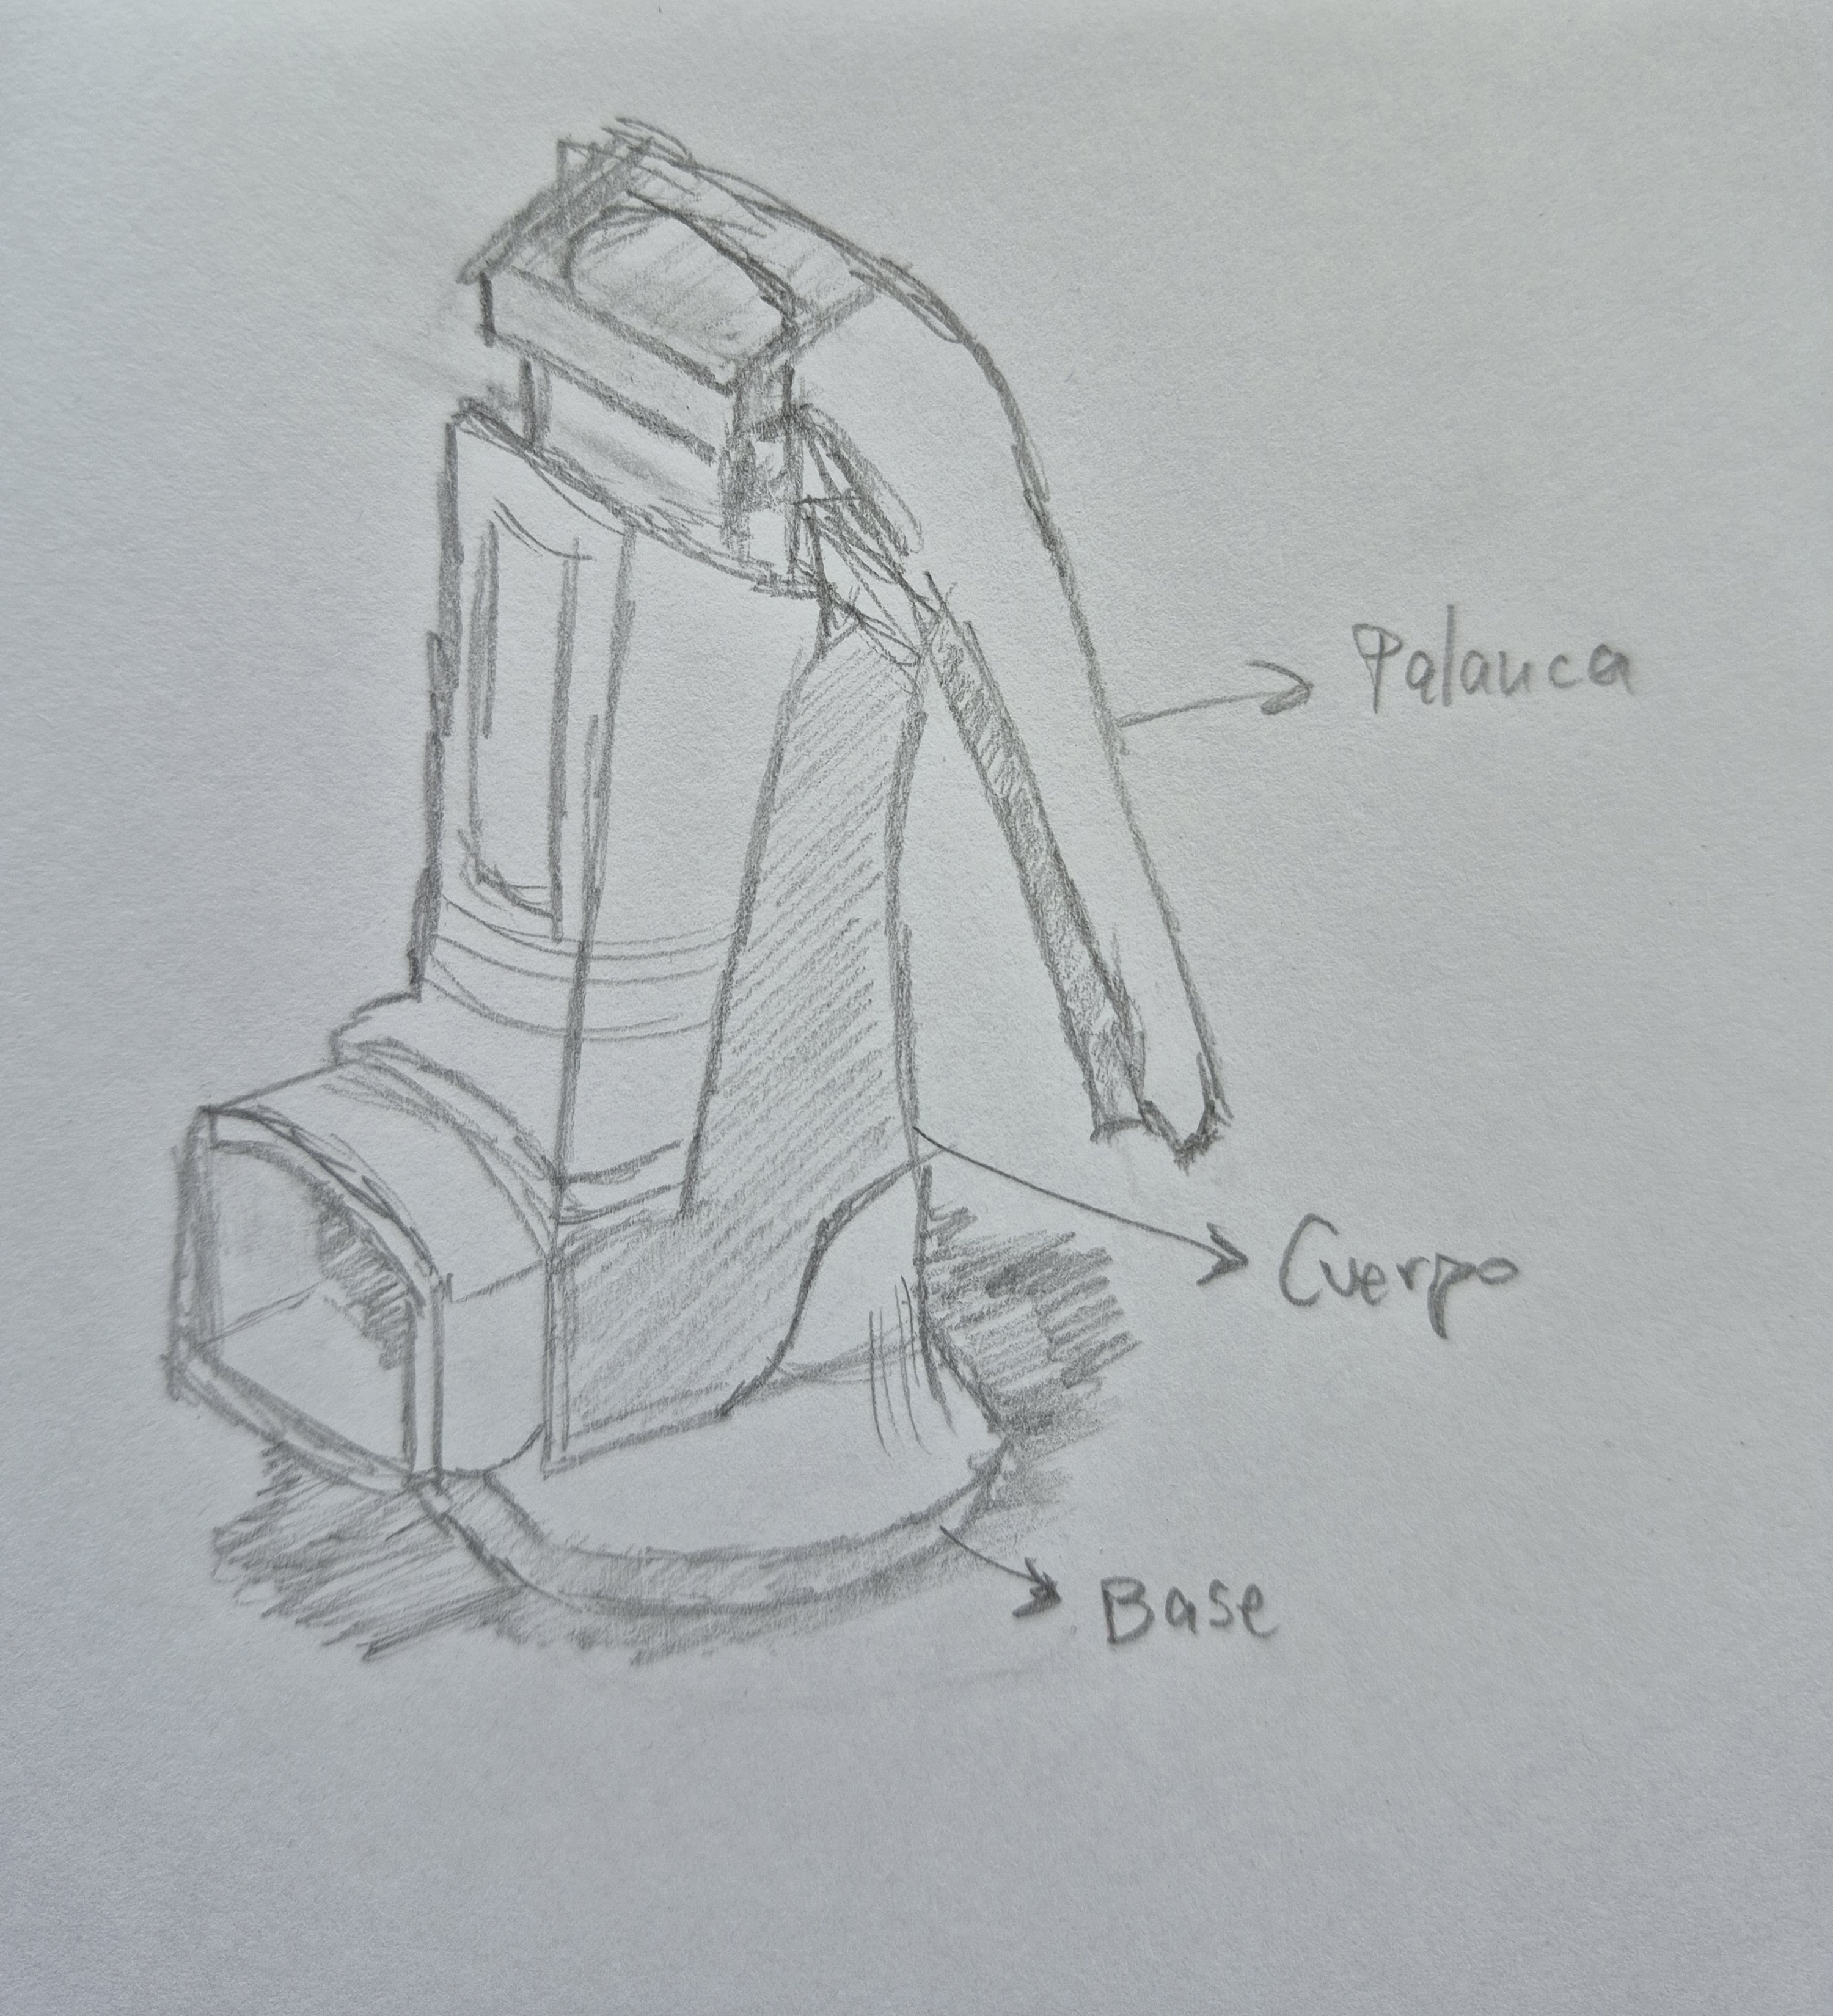
\includegraphics[width=0.8\textwidth]{boceto_antonio_1.jpg}
    \caption{Boceto preliminar 1 - D. Antonio Sánchez Doña.}
    \label{fig:boceto_antonio_1}
\end{figure}

\vspace{0.5cm}

\begin{figure}[H]
    \centering
    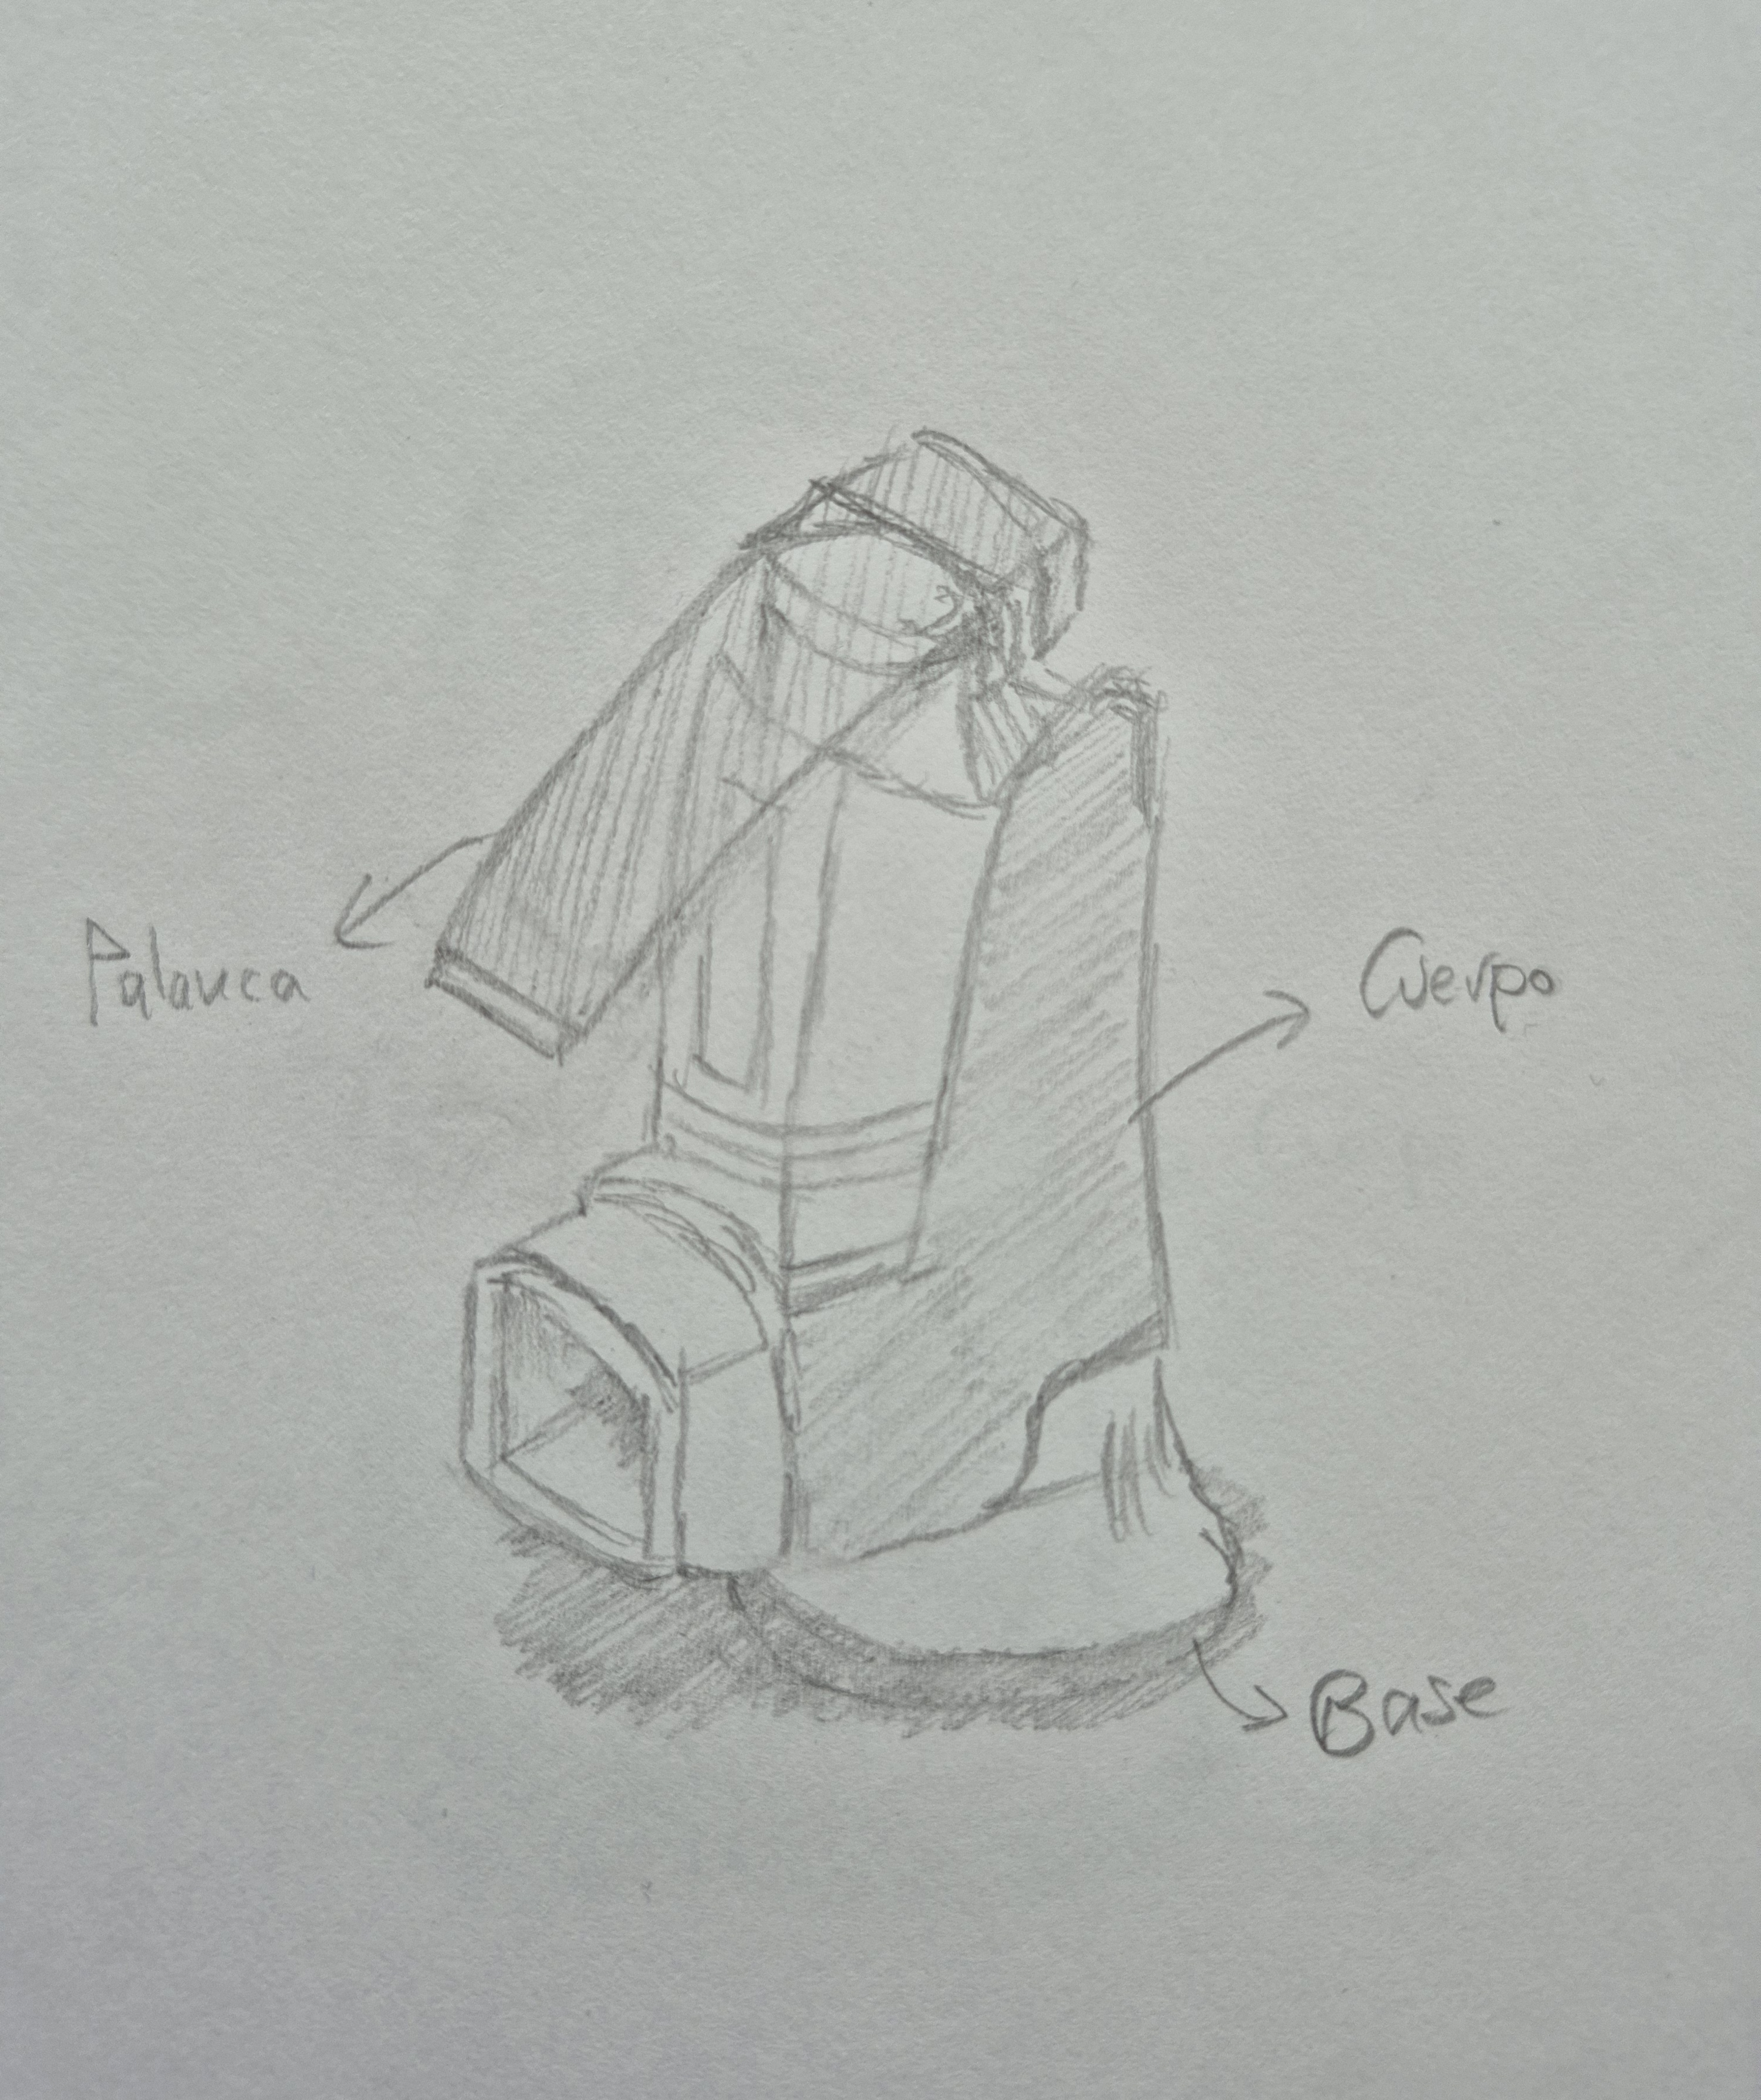
\includegraphics[width=0.8\textwidth]{boceto_antonio_2.jpg}
    \caption{Boceto preliminar 2 - D. Antonio Sánchez Doña.}
    \label{fig:boceto_antonio_2}
\end{figure}

\begin{figure}[H]
    \centering
    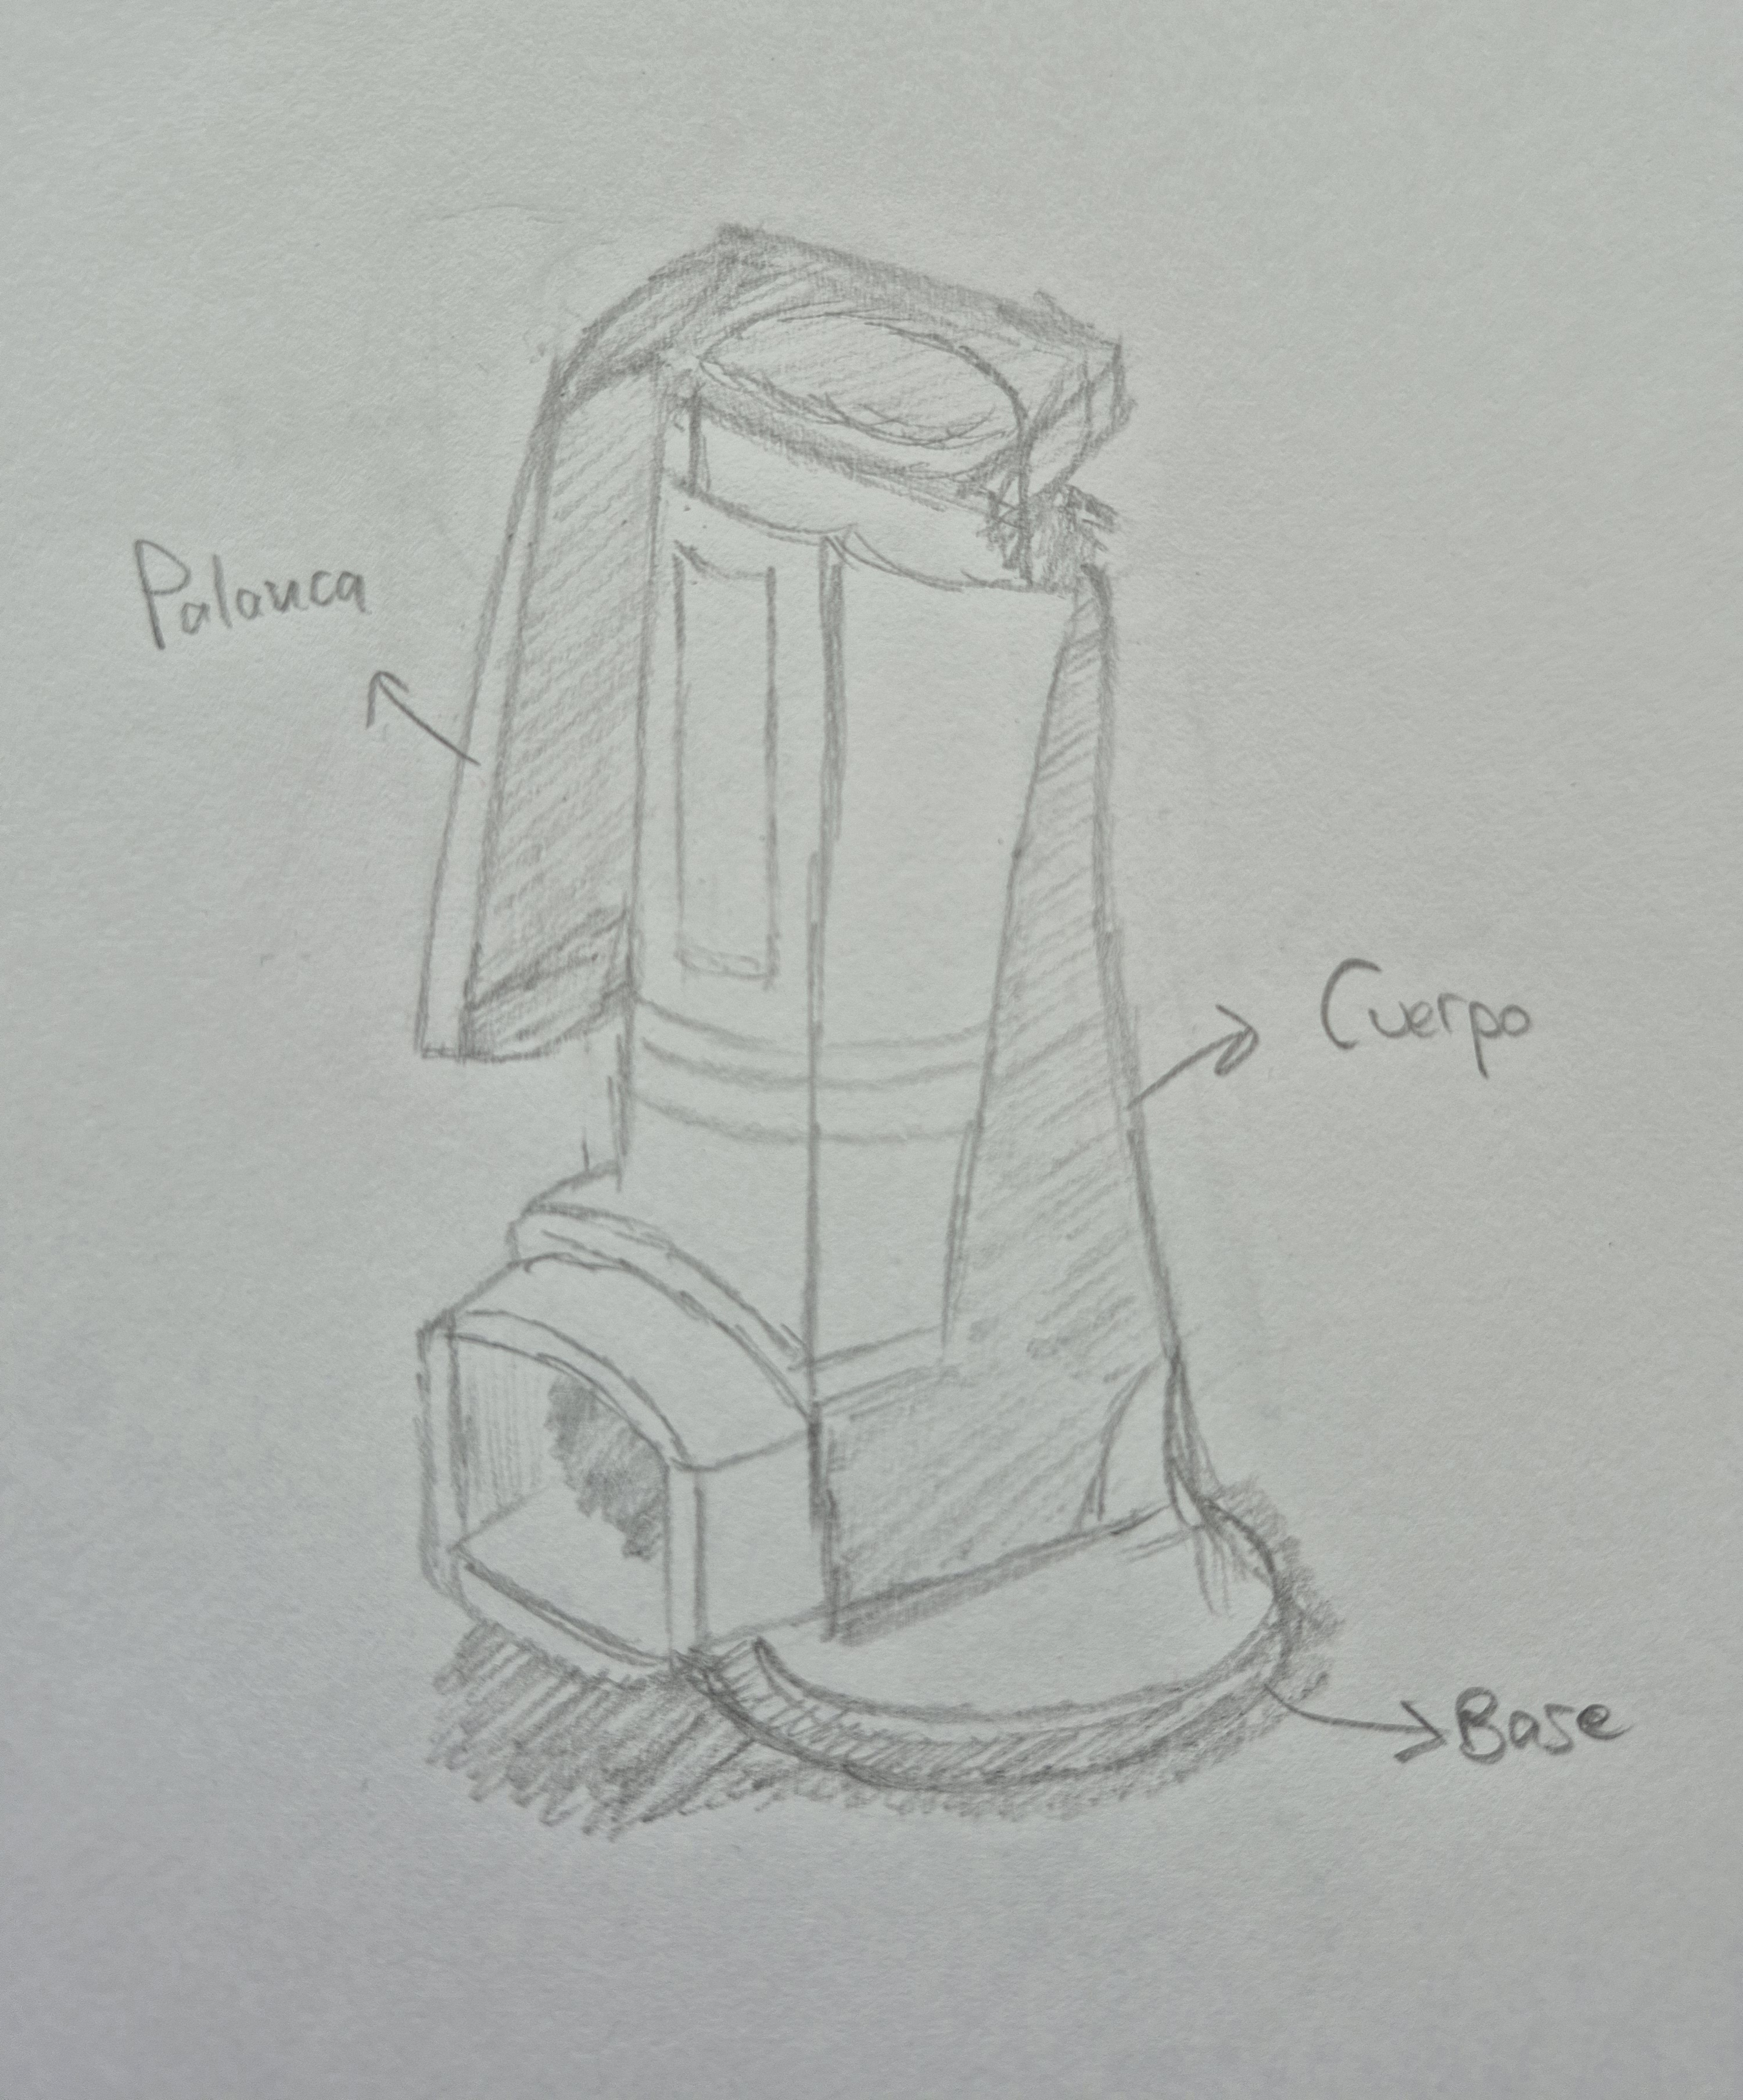
\includegraphics[width=0.8\textwidth]{boceto_antonio_3.jpg}
    \caption{Boceto preliminar 3 - D. Antonio Sánchez Doña.}
    \label{fig:boceto_antonio_3}
\end{figure}

\vspace{0.5cm}

\begin{figure}[H]
    \centering
    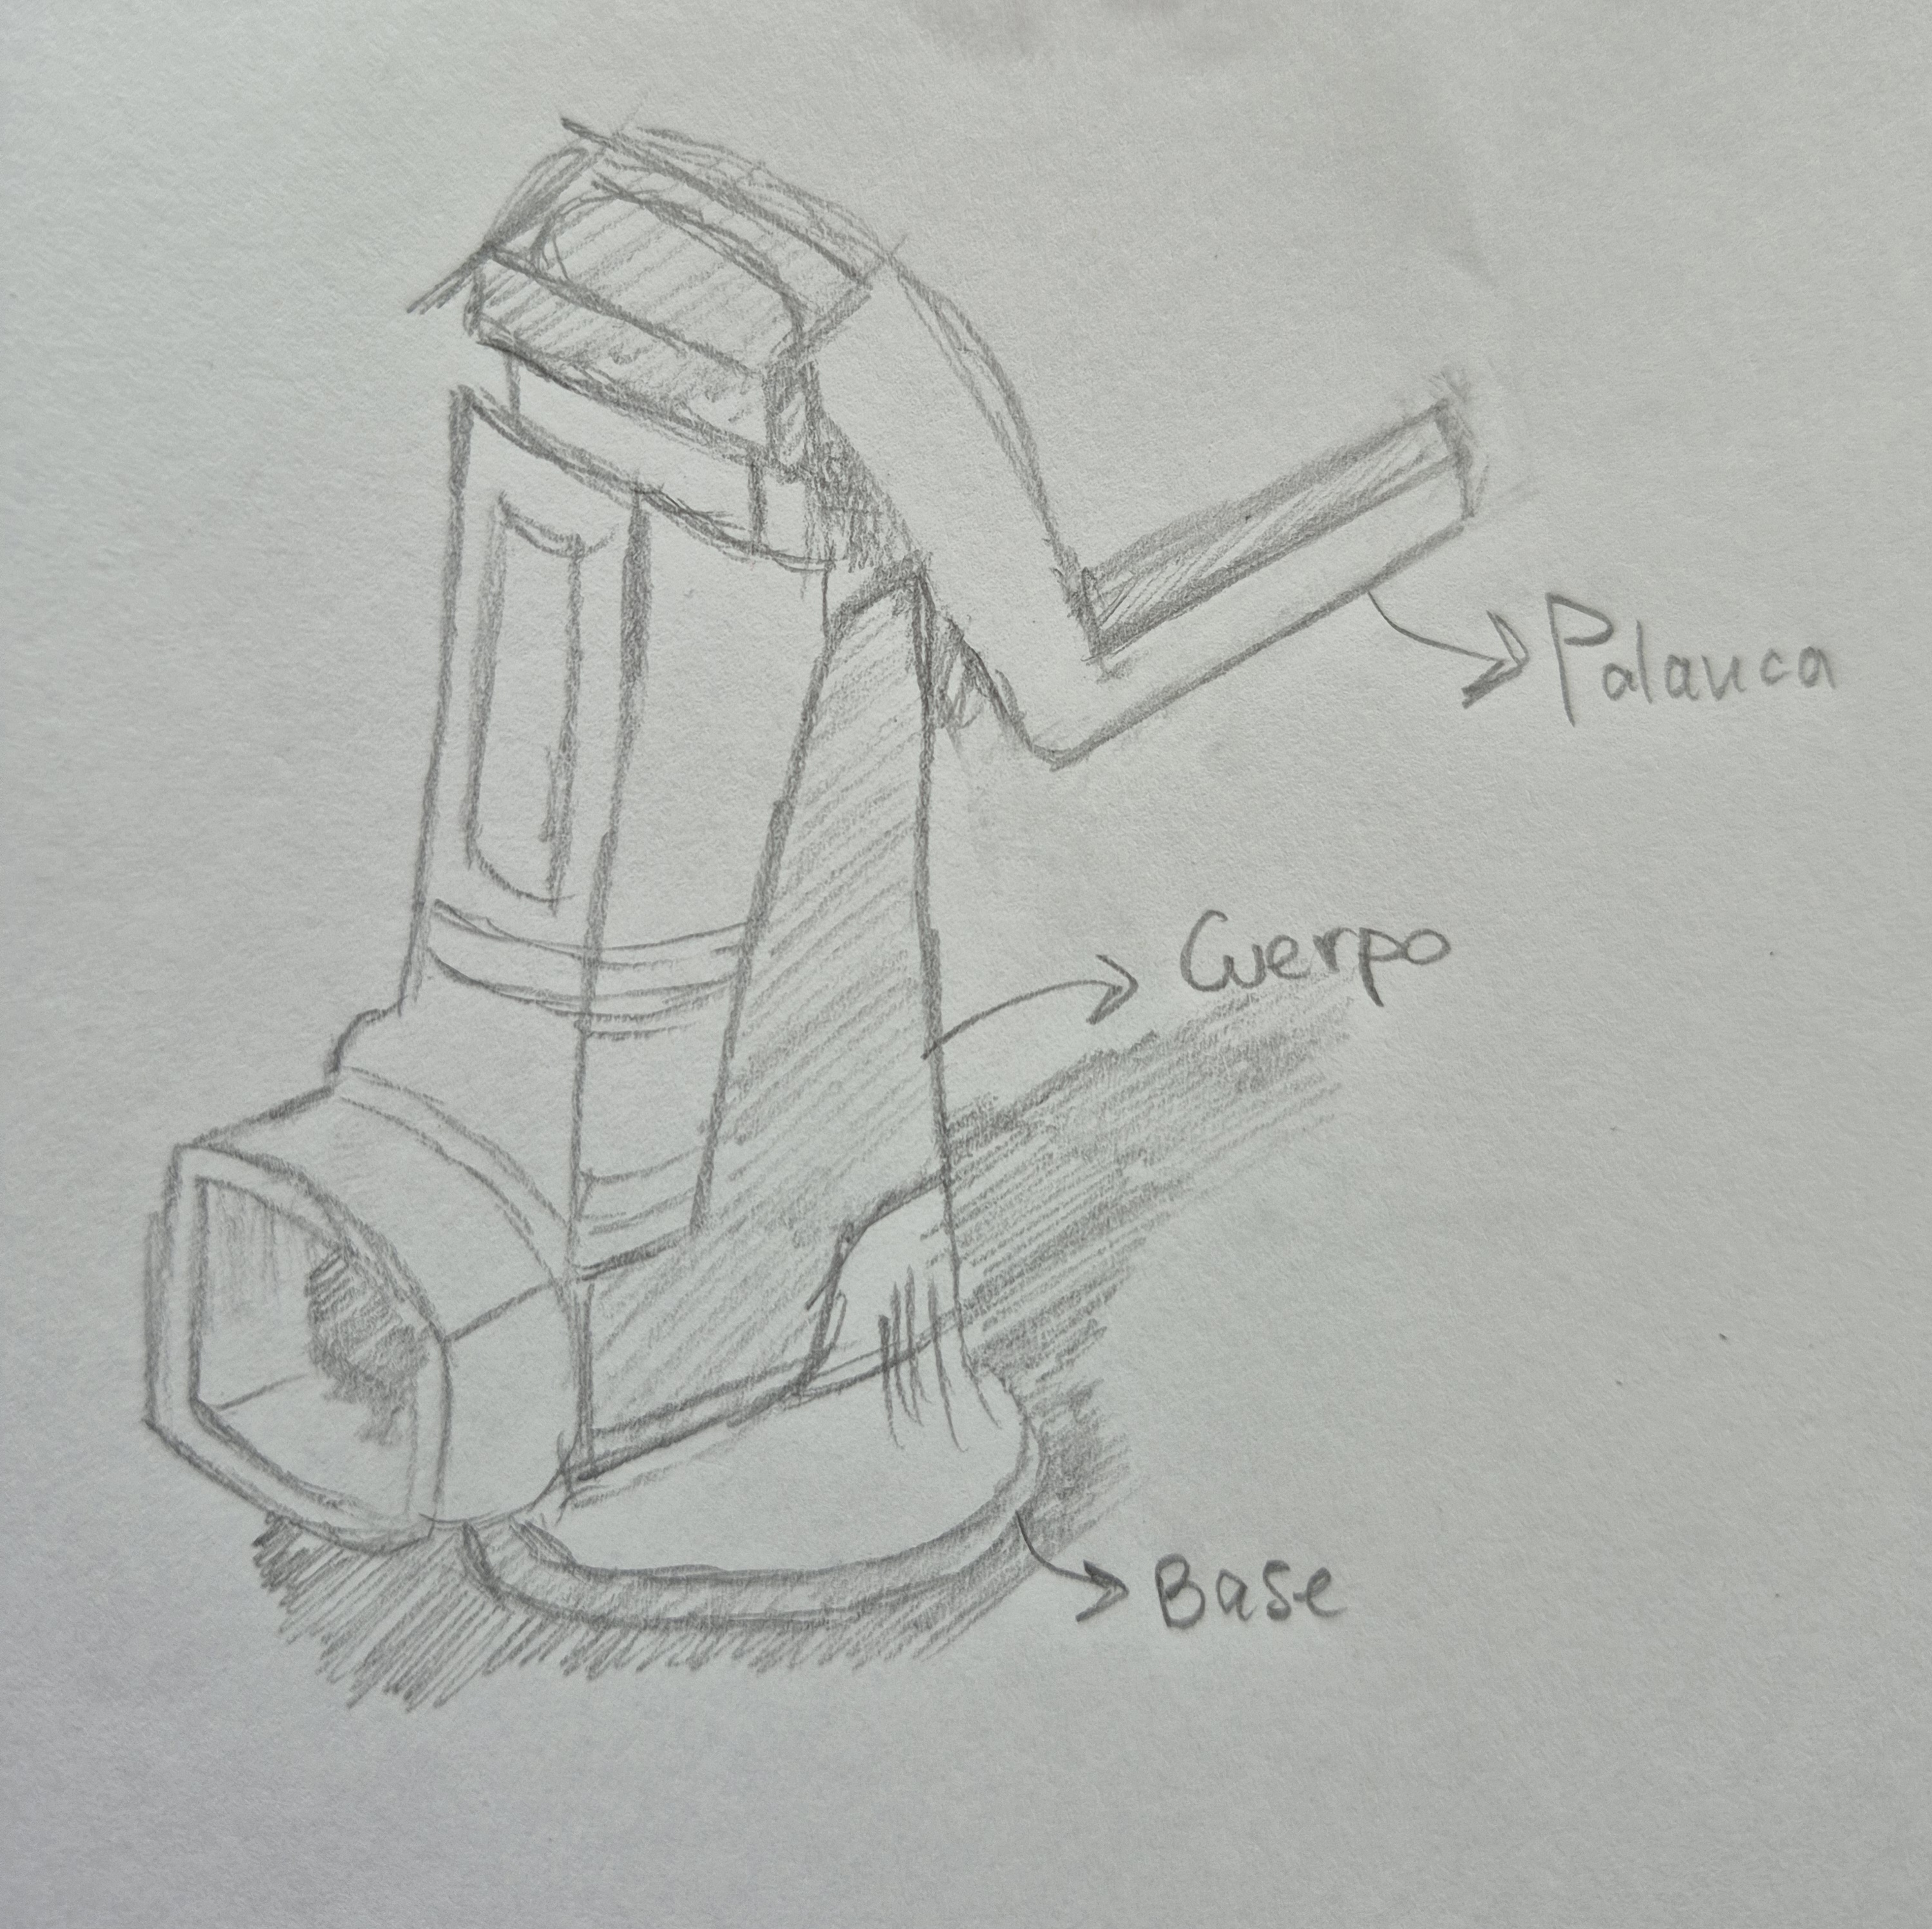
\includegraphics[width=0.8\textwidth]{boceto_antonio_4.jpg}
    \caption{Boceto preliminar 4 - D. Antonio Sánchez Doña.}
    \label{fig:boceto_antonio_4}
\end{figure}

\begin{figure}[H]
    \centering
    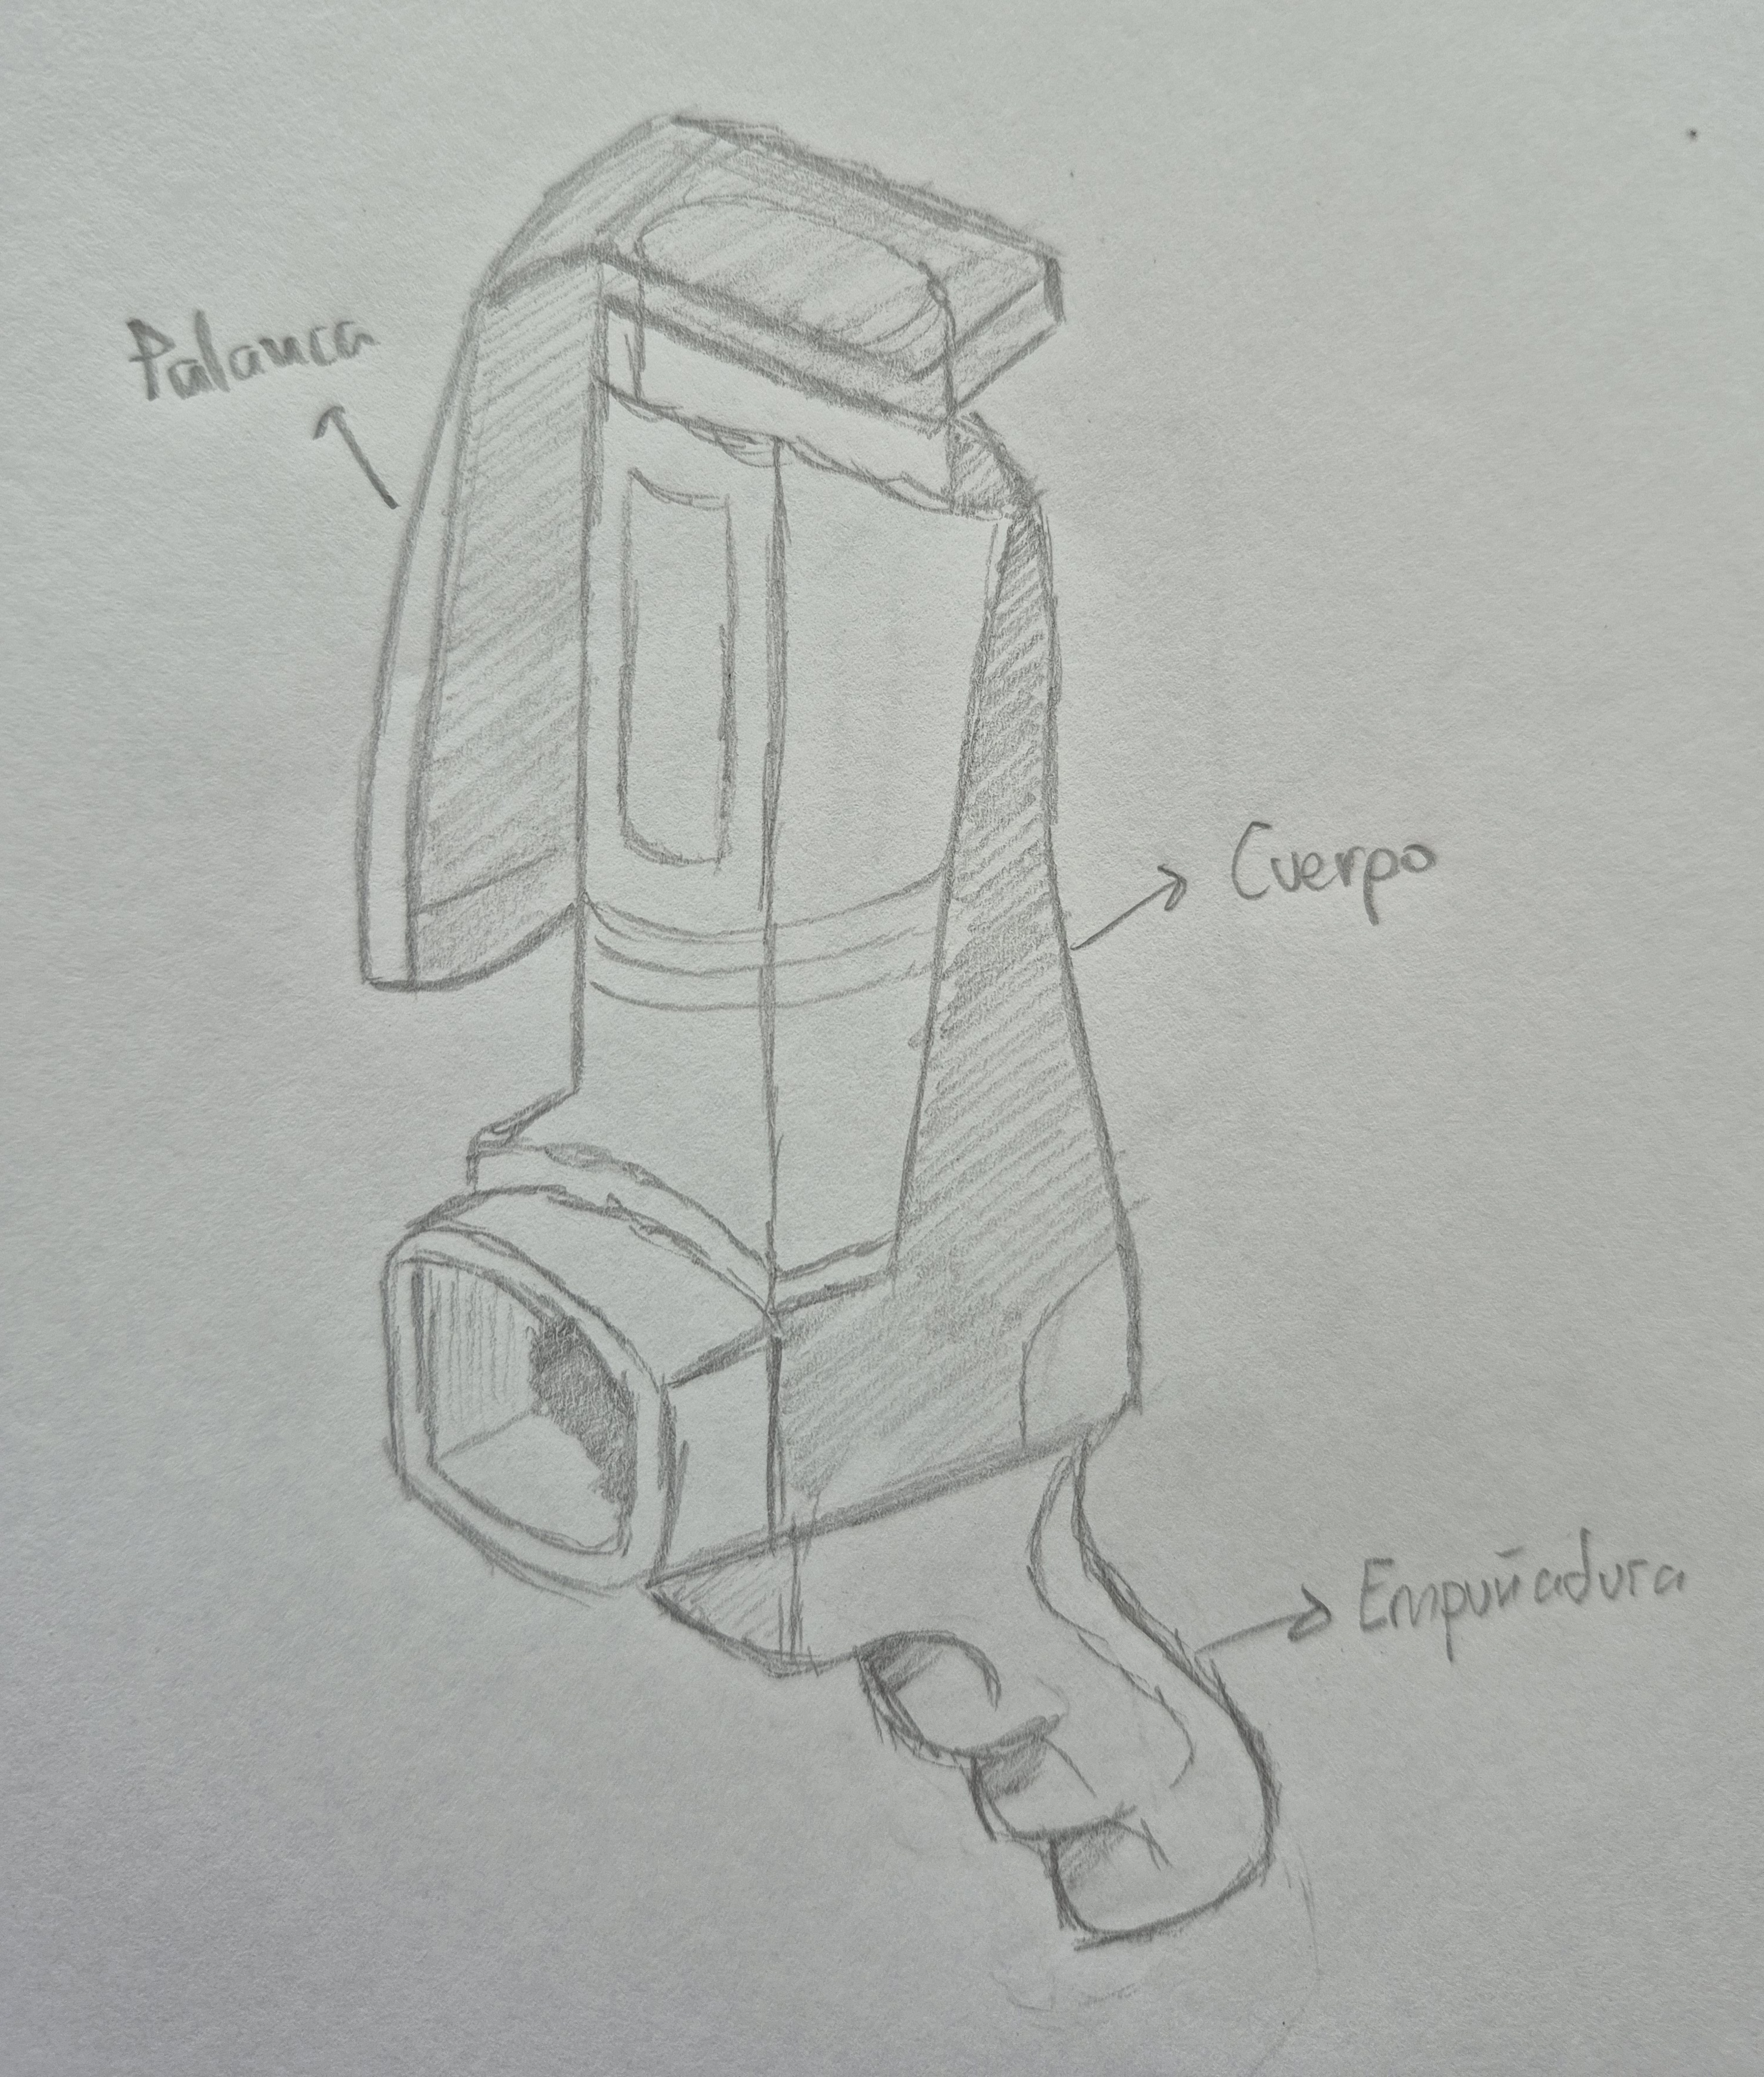
\includegraphics[width=0.8\textwidth]{boceto_antonio_5.jpg}
    \caption{Boceto preliminar 5 - D. Antonio Sánchez Doña.}
    \label{fig:boceto_antonio_5}
\end{figure}

\newpage

% ------------------------------------------------------
% BOCETOS SERGIO
% ------------------------------------------------------
\subsection{Bocetos realizados por el proyectista D. Sergio Carmona Muñoz}

\begin{figure}[H]
    \centering
    
\includegraphics[width=0.8\textwidth]{ANEXOS/Boceto1_SCM.jpeg}
    \caption{Boceto preliminar 6 - D. Sergio Carmona Muñoz.}
    \label{fig:boceto_sergio_1}
\end{figure}

\vspace{0.5cm}

\begin{figure}[H]
    \centering
    
\includegraphics[width=0.8\textwidth]{ANEXOS/Boceto2_SCM.jpeg}
    \caption{Boceto preliminar 7 - D. Sergio Carmona Muñoz.}
    \label{fig:boceto_sergio_2}
\end{figure}

\begin{figure}[H]
    \centering
    
\includegraphics[width=0.8\textwidth]{ANEXOS/Boceto3_SCM.jpeg}
    \caption{Boceto preliminar 8 - D. Sergio Carmona Muñoz.}
    \label{fig:boceto_sergio_3}
\end{figure}

\vspace{0.5cm}

\begin{figure}[H]
    \centering
    
\includegraphics[width=0.8\textwidth]{ANEXOS/Boceto4_SCM.jpeg}
    \caption{Boceto preliminar 9 - D. Sergio Carmona Muñoz.}
    \label{fig:boceto_sergio_4}
\end{figure}

\begin{figure}[H]
    \centering
    
\includegraphics[width=0.8\textwidth]{ANEXOS/Boceto5_SCM.jpeg}
    \caption{Boceto preliminar 10 - D. Sergio Carmona Muñoz.}
    \label{fig:boceto_sergio_5}
\end{figure}

\newpage

% ------------------------------------------------------
% BOCETOS JUAN GABRIEL
% ------------------------------------------------------
\subsection{Bocetos realizados por el proyectista D. Juan Gabriel Navarro}

\begin{figure}[H]
    \centering
    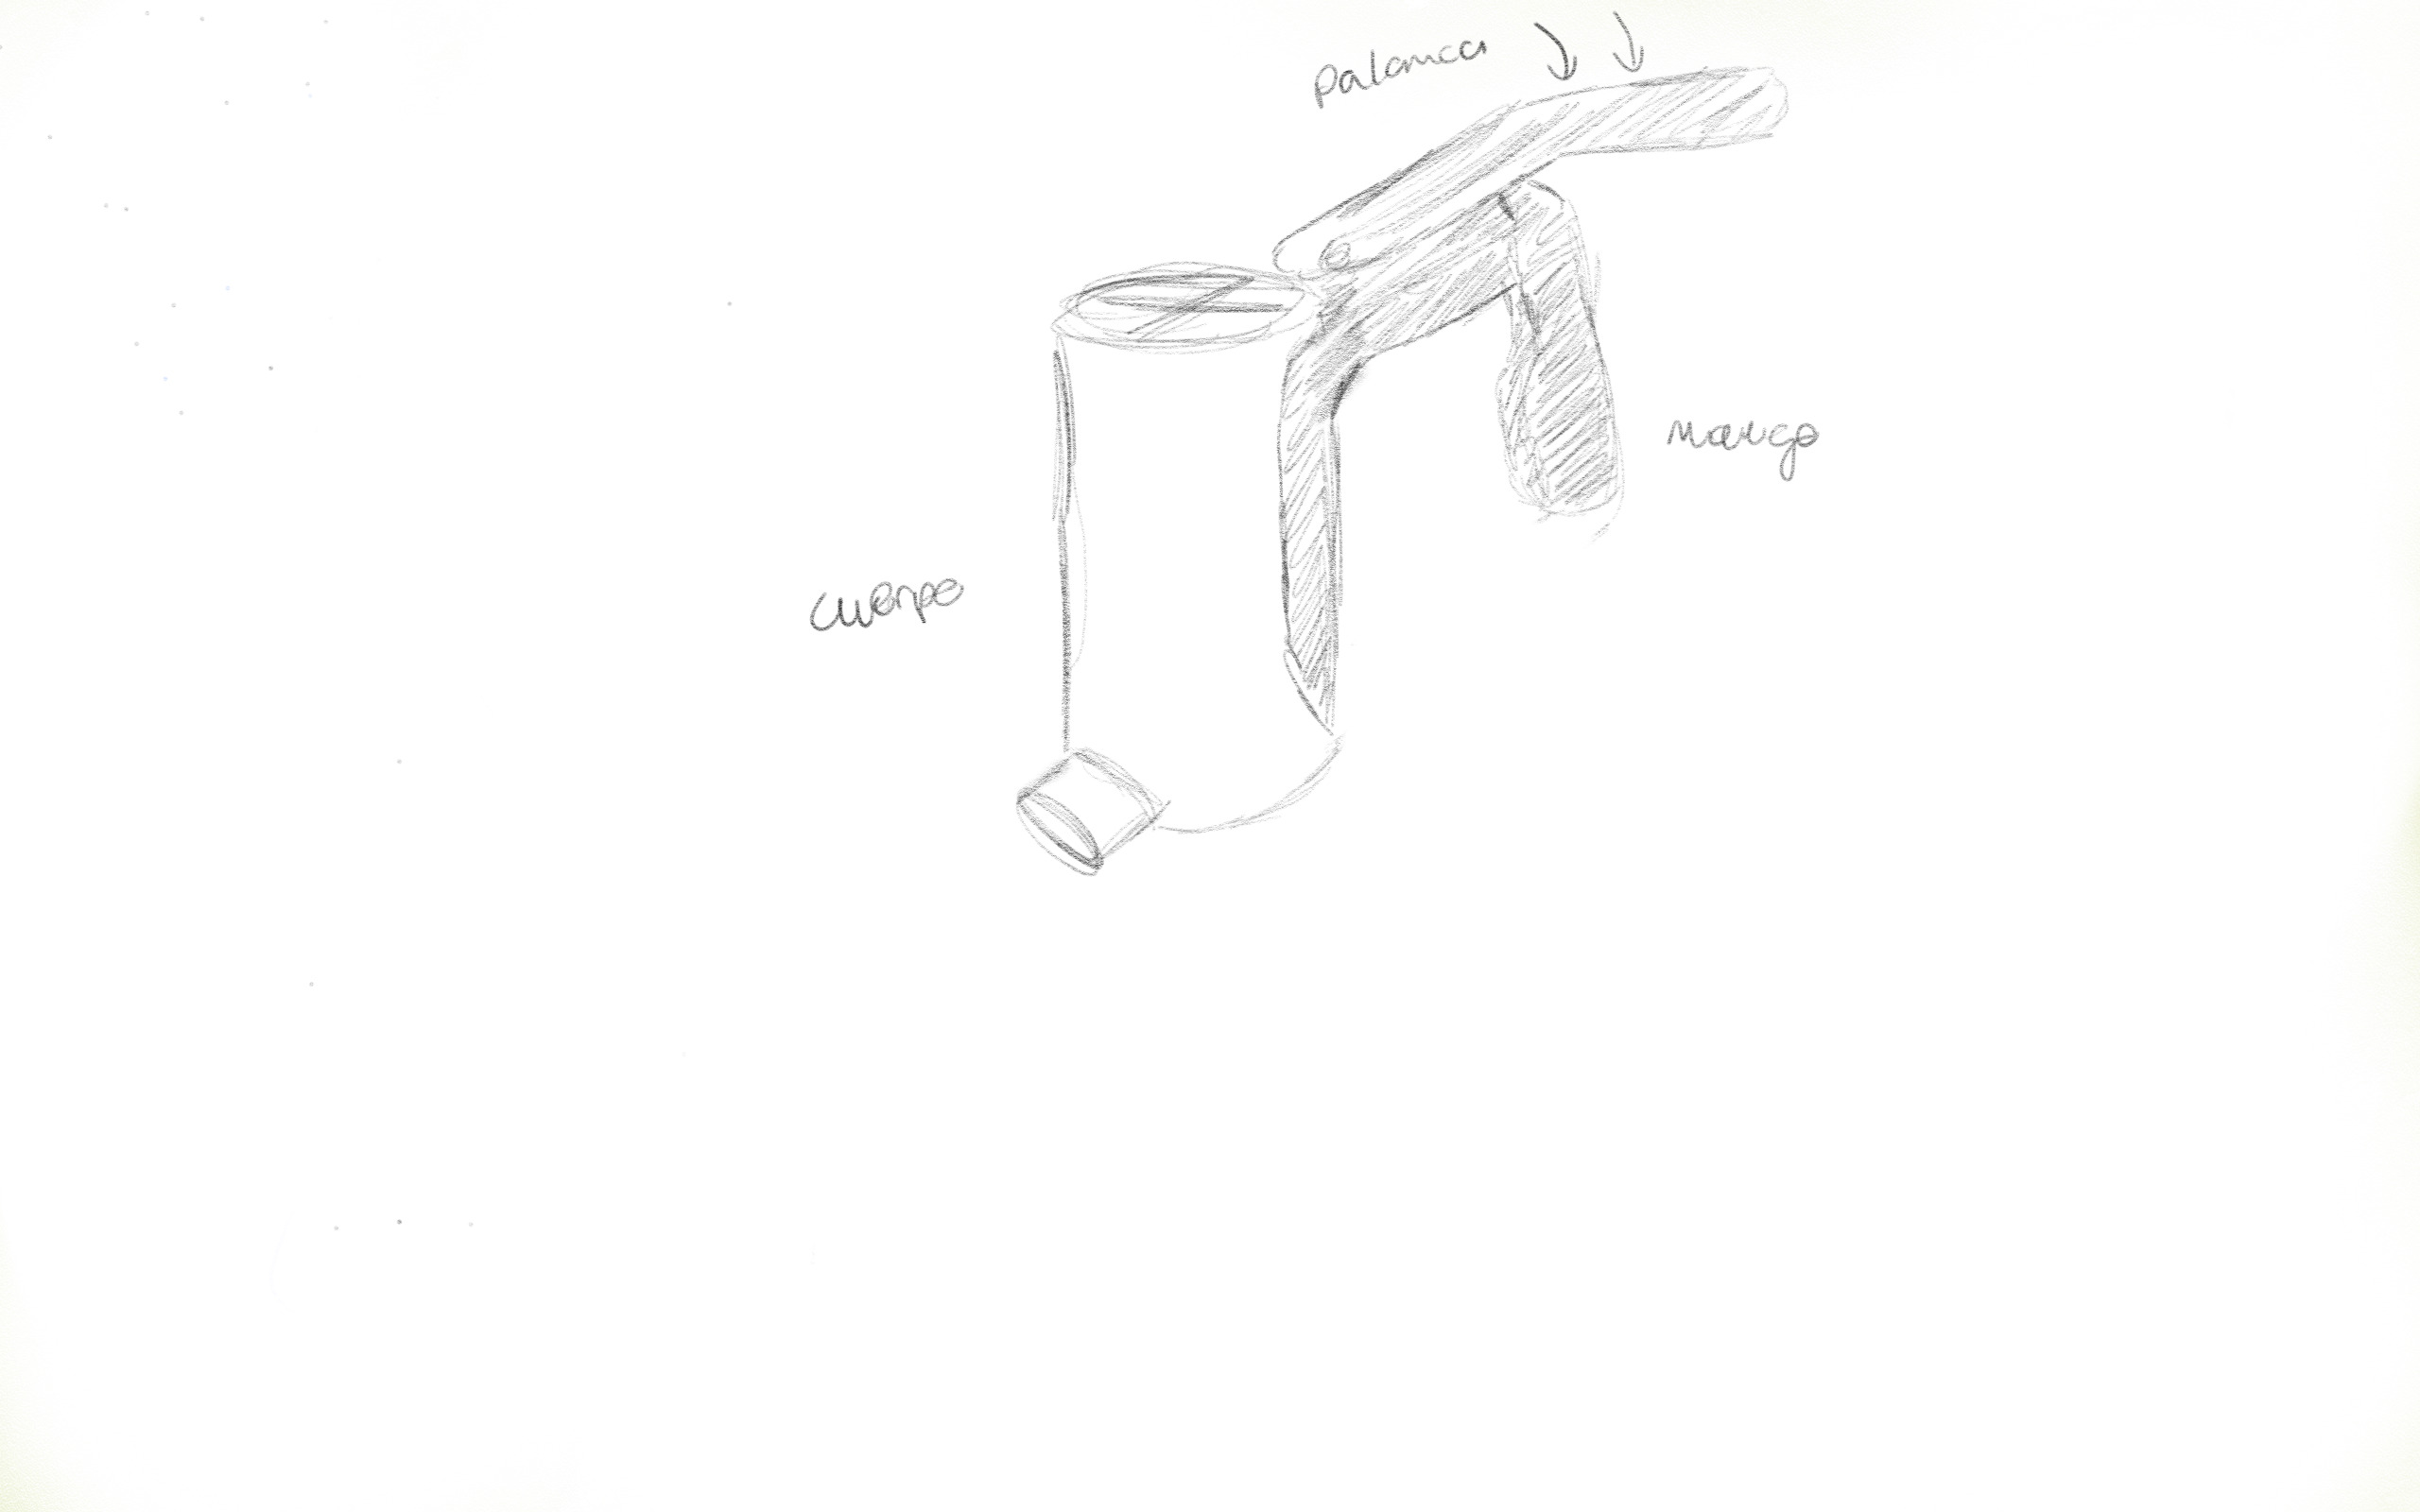
\includegraphics[width=0.8\textwidth]{boceto_juan_1.jpg}
    \caption{Boceto preliminar 11 - D. Juan Gabriel Navarro Valdivielso.}
    \label{fig:boceto_juan_1}
\end{figure}

\vspace{0.5cm}

\begin{figure}[H]
    \centering
    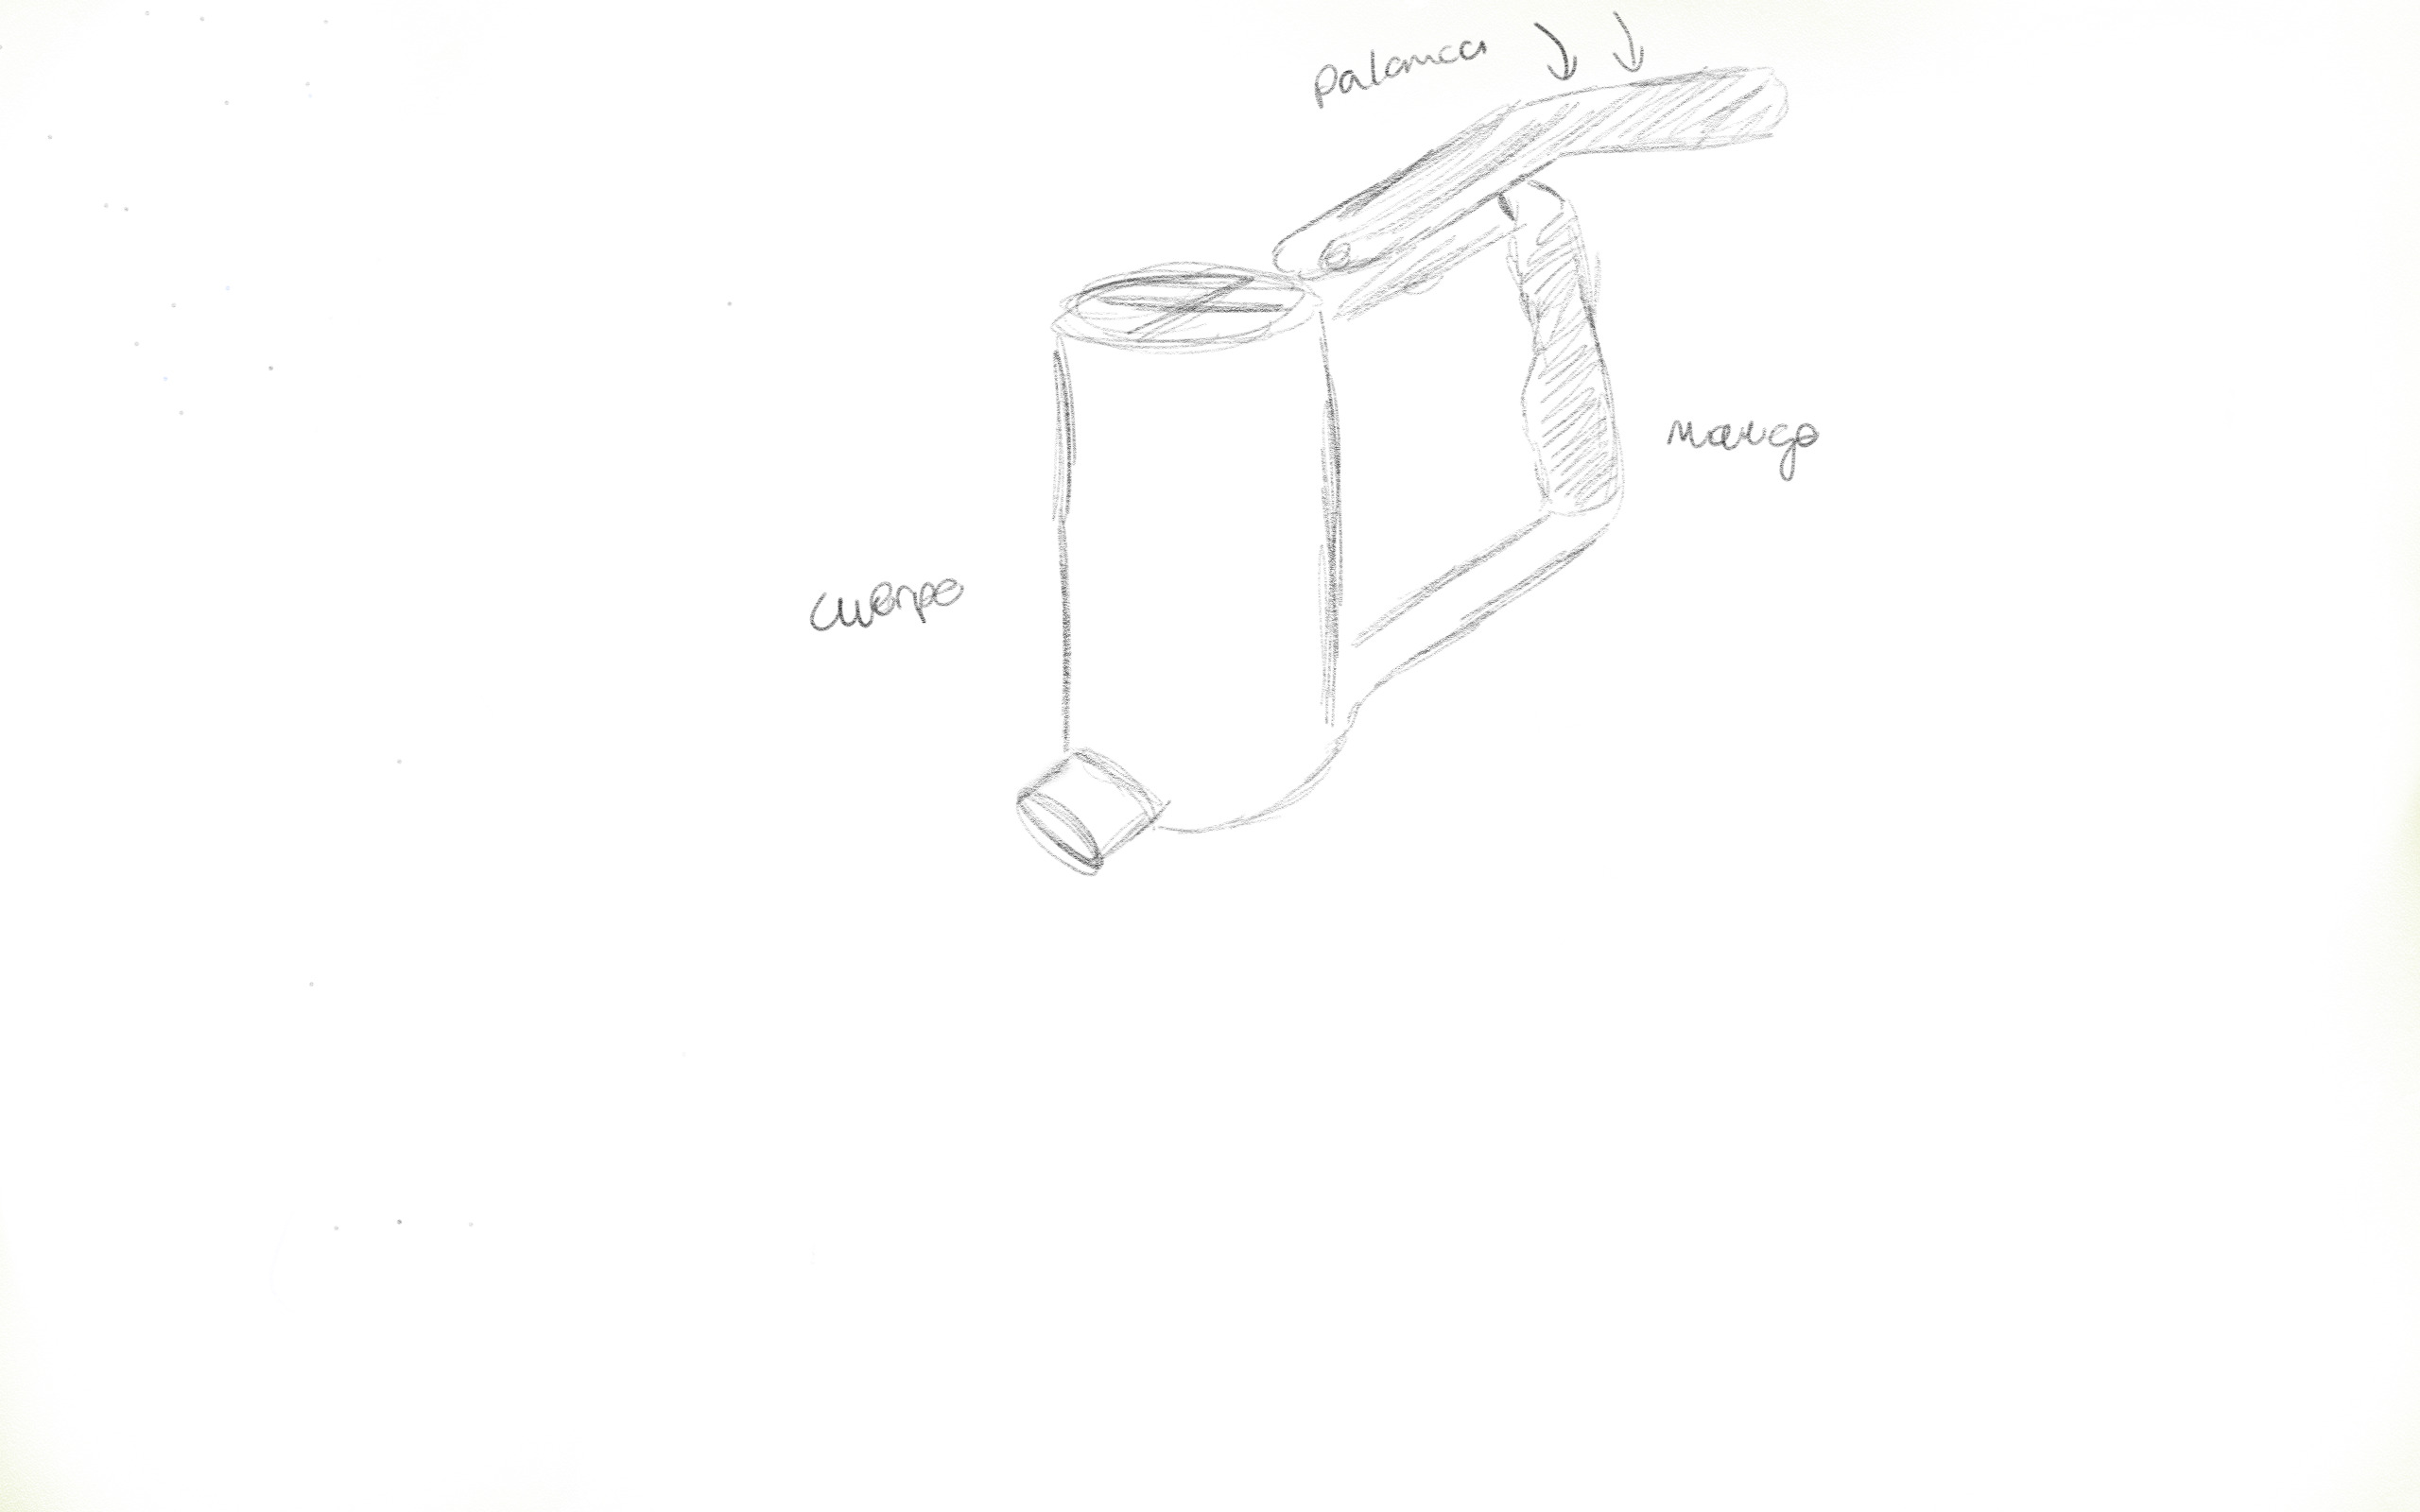
\includegraphics[width=0.8\textwidth]{boceto_juan_2.jpg}
    \caption{Boceto preliminar 12 - D. Juan Gabriel Navarro Valdivielso.}
    \label{fig:boceto_juan_2}
\end{figure}

\begin{figure}[H]
    \centering
    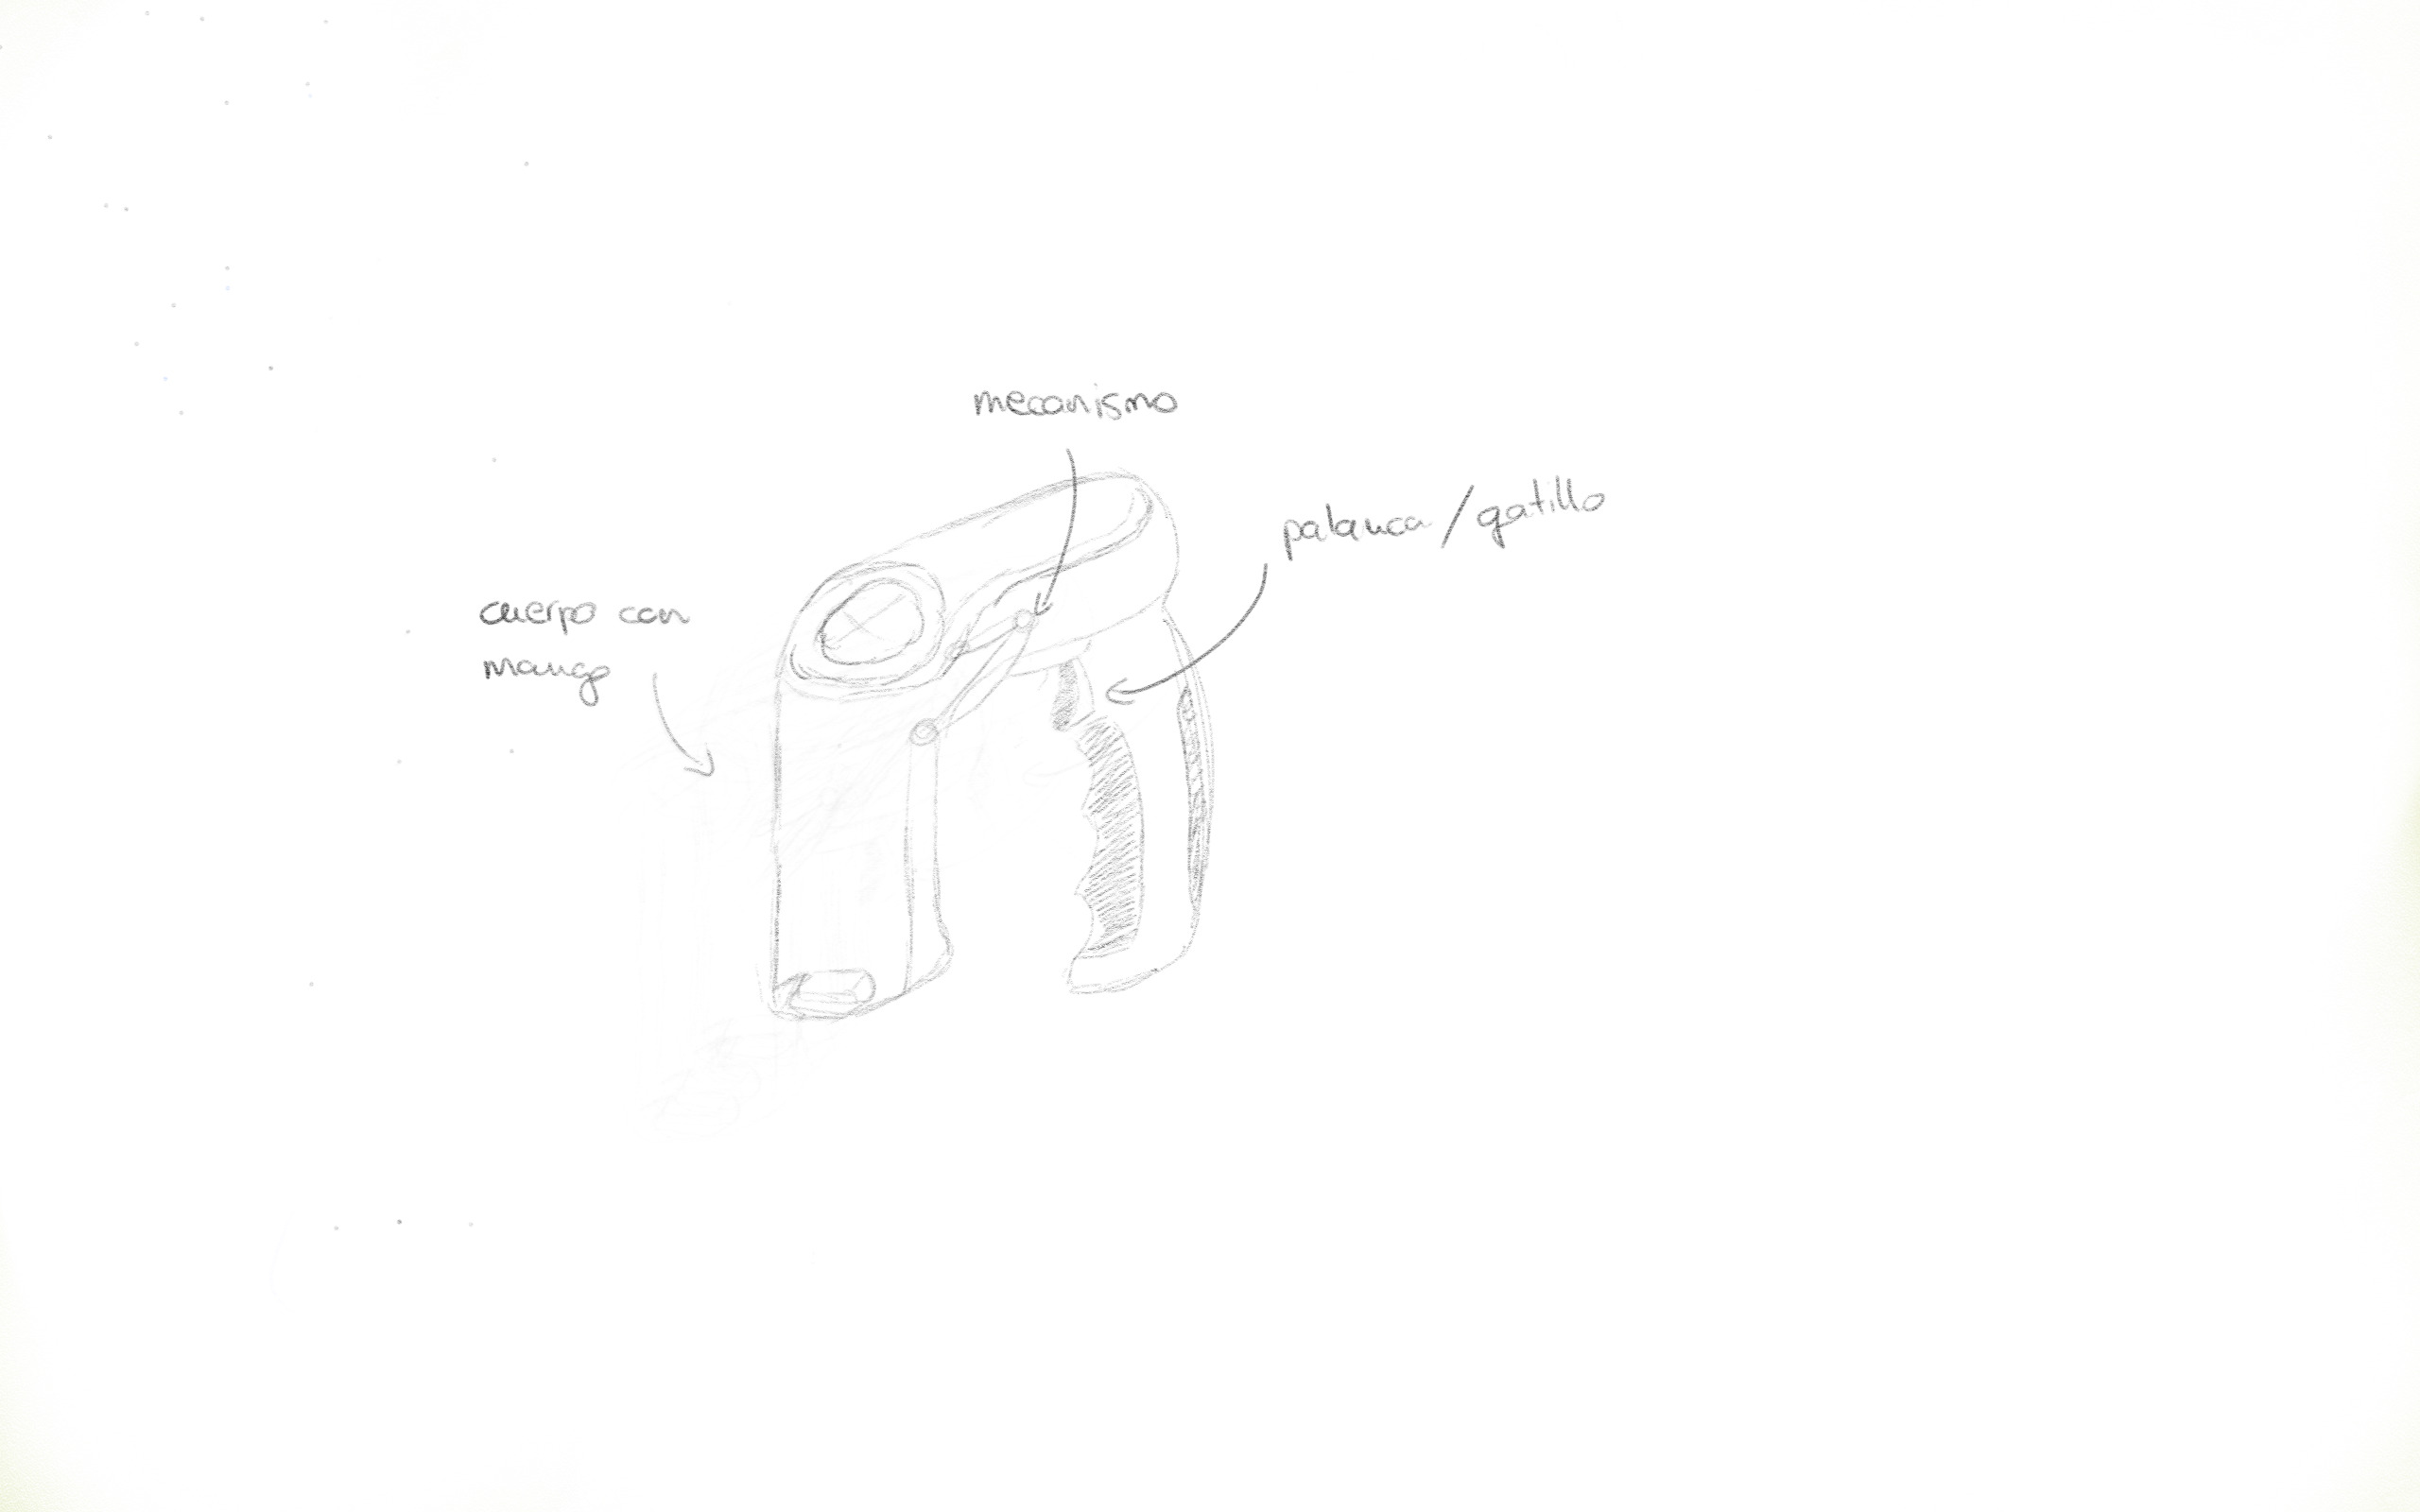
\includegraphics[width=0.8\textwidth]{boceto_juan_3.jpg}
    \caption{Boceto preliminar 13 - D. Juan Gabriel Navarro Valdivielso.}
    \label{fig:boceto_juan_3}
\end{figure}

\vspace{0.5cm}

\begin{figure}[H]
    \centering
    
\includegraphics[width=0.8\textwidth]{boceto_juan_4.jpg}
    \caption{Boceto preliminar 14 - D. Juan Gabriel Navarro Valdivielso.}
    \label{fig:boceto_juan_4}
\end{figure}

\begin{figure}[H]
    \centering
    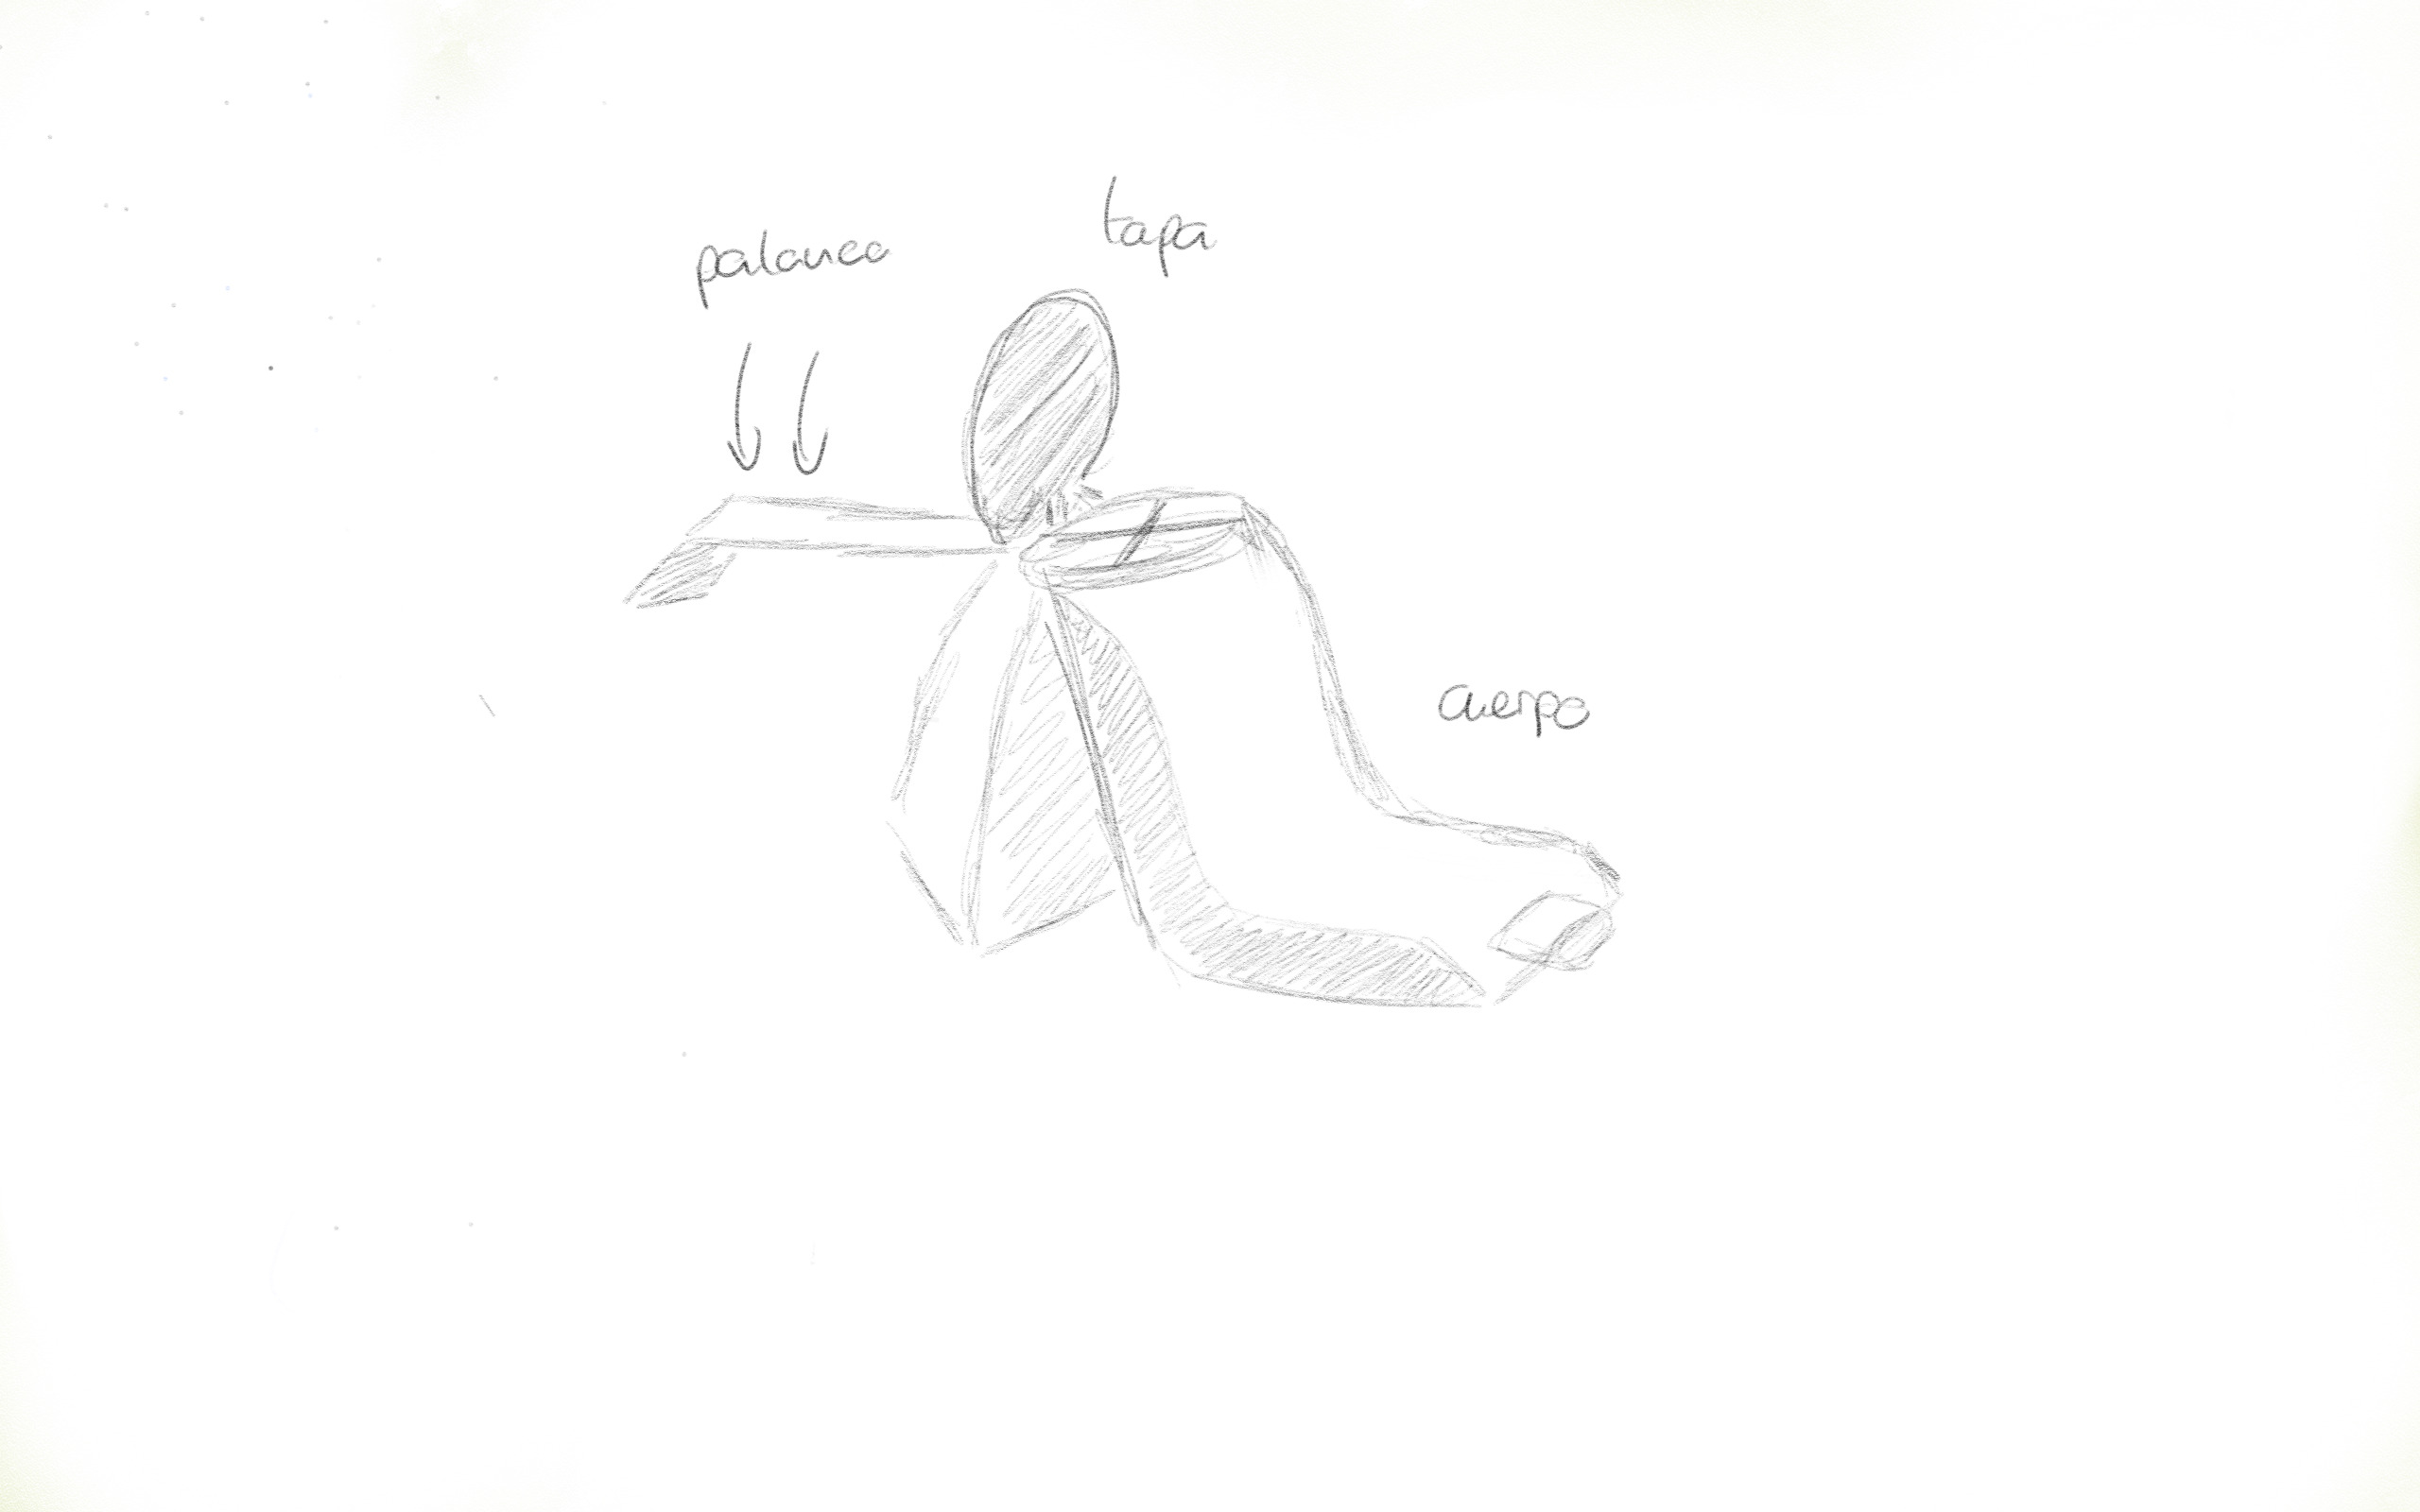
\includegraphics[width=0.8\textwidth]{boceto_juan_5.jpg}
    \caption{Boceto preliminar 15 - D. Juan Gabriel Navarro Valdivielso.}
    \label{fig:boceto_juan_5}
\end{figure}

\newpage



% ------------------------------------------------------
% BOCETOS IVÁN
% ------------------------------------------------------
\subsection{Bocetos realizados por el proyectista D. Iván de la Torre Segato}

\begin{figure}[H]
    \centering
    
\includegraphics[width=0.8\textwidth]{ANEXOS/Boceto1_Iván.jpeg}
    \caption{Boceto preliminar 16 - D. Iván de la Torre Segato.}
    \label{fig:boceto_ivan_1}
\end{figure}

\vspace{0.5cm}

\begin{figure}[H]
    \centering
    
\includegraphics[width=0.8\textwidth]{ANEXOS/Boceto2_Iván.jpeg}
    \caption{Boceto preliminar 17 - D. Iván de la Torre Segato.}
    \label{fig:boceto_ivan_2}
\end{figure}

\begin{figure}[H]
    \centering
    
\includegraphics[width=0.8\textwidth]{ANEXOS/Boceto3_Iván.jpeg}
    \caption{Boceto preliminar 18 - D. Iván de la Torre Segato.}
    \label{fig:boceto_ivan_3}
\end{figure}

\vspace{0.5cm}

\begin{figure}[H]
    \centering
    
\includegraphics[width=0.8\textwidth]{ANEXOS/Boceto4_Iván.jpeg}
    \caption{Boceto preliminar 19 - D. Iván de la Torre Segato.}
    \label{fig:boceto_ivan_4}
\end{figure}

\begin{figure}[H]
    \centering
    
\includegraphics[width=0.8\textwidth]{ANEXOS/Boceto5_Iván.jpeg}
    \caption{Boceto preliminar 20 - D. Iván de la Torre Segato.}
    \label{fig:boceto_ivan_5}
\end{figure}

\newpage



% ======================================================
% MATRIZ DE EVALUACIÓN Y SELECCIÓN DE DISEÑO
% ======================================================

\section{Matriz de evaluación y selección de diseño}


\nopagebreak
\begin{table}[H]
    \centering
    \small
    \renewcommand{\arraystretch}{1.4} % Mayor holgura vertical para lectura cómoda
    \renewcommand{\tabularxcolumn}[1]{m{#1}} % <--- SOLUCIÓN: Centra verticalmente todas las columnas X
    \begin{tabularx}{\linewidth}{>{\color{ArthroNavy}\bfseries\centering\arraybackslash}m{2.2cm} X}
        \hline
        \rowcolor{ArthroNavy}
        \color{white}\textbf{Criterio} & \multicolumn{1}{>{\centering\arraybackslash}X}{\color{white}\textbf{Definición Técnica y Funcional}} \\ \hline
        
        \rowcolor{ArthroTeal!5}
        A & \textbf{Ergonomía de accionamiento:} El diseño visual sugiere la capacidad de sustituir el movimiento de pinza por empuje palmar para reducir el esfuerzo. \\
        
        B & \textbf{Facilidad de montaje/desmontaje:} La geometría propuesta parece permitir un ensamblaje intuitivo sin necesidad de herramientas ni movimientos finos. \\
        
        \rowcolor{ArthroTeal!5}
        C & \textbf{Confort y seguridad de agarre:} Presencia de superficies redondeadas, zonas amplias de contacto y posibles texturas antideslizantes. \\
        
        D & \textbf{Viabilidad geométrica de fabricación:} Diseño simplificado que apunte a un fácil desmoldeo (o fabricación 3D) sin contrasalidas excesivas. \\
        
        \rowcolor{ArthroTeal!5}
        E & \textbf{Facilidad de limpieza:} Acceso visual y físico abierto a la cavidad interior, evitando el diseño de recovecos donde se acumule suciedad. \\
        
        F & \textbf{Uso autónomo a una mano:} La disposición de las piezas permite deducir que el usuario podría operar el dispositivo de forma independiente. \\
        
        \rowcolor{ArthroTeal!5}
        G & \textbf{Estética e identidad visual:} Aspecto general del boceto diferenciado de los competidores directos, manteniendo un carácter discreto y médico. \\ \hline
    \end{tabularx}
    \caption{Definición de los criterios técnicos y funcionales de evaluación cualitativa empleados en la Matriz de selección de conceptos (Matriz de Pugh) para evaluar las alternativas generadas.}
    \label{tab:criterios_evaluacion}
\end{table}

\vspace{0.3cm}


\vspace{0.5cm}

\begin{landscape}
\vspace*{\fill}
\begin{table}[H]
    \centering
    % Mantenemos el estirado vertical para dar espacio a la fuente
    \renewcommand{\arraystretch}{2.8} 
    \setlength{\tabcolsep}{5pt} 
    
    % Escalamos al ancho de la página
    \resizebox{\linewidth}{!}{
    \large 
    % Cambiamos la primera columna de 'c' a 'm{7cm}' para permitir texto largo en varias líneas
    \begin{tabular}{|>{\bfseries\huge\centering\arraybackslash}m{7cm}|c|c|c|c|c|c|c|c|c|c|c|c|c|c|c|c|c|c|c|c|}
        \hline
        % Fila 1: Ajustamos la caja diagonal al nuevo ancho de la columna (7.4cm para compensar bordes)
        \multirow{3}{*}{\diagbox[width=7.4cm, height=5cm]{\textbf{\huge Criterio}}{\textbf{\huge Concepto}}} &
        \textbf{\huge ASD} & \textbf{\huge ASD} & \textbf{\huge ASD} & \textbf{\huge ASD} & \textbf{\huge ASD} & \textbf{\huge SCM} & \textbf{\huge SCM} & \textbf{\huge SCM} & \textbf{\huge SCM} & \textbf{\huge SCM} & \textbf{\huge JGN} & \textbf{\huge JGN} & \textbf{\huge JGN} & \textbf{\huge JGN} & \textbf{\huge JGN} & \textbf{\huge ITS} & \textbf{\huge ITS} & \textbf{\huge ITS} & \textbf{\huge ITS} & \textbf{\huge ITS} \\ \cline{2-21}
        
        % Fila 2: Números en tamaño Huge
        & \textbf{\huge 1} & \textbf{\huge 2} & \textbf{\huge 3} & \textbf{\huge 4} & \textbf{\huge 5} & \textbf{\huge 6} & \textbf{\huge 7} & \textbf{\huge 8} & \textbf{\huge 9} & \textbf{\huge 10} & \textbf{\huge 11} & \textbf{\huge 12} & \textbf{\huge 13} & \textbf{\huge 14} & \textbf{\huge 15} & \textbf{\huge 16} & \textbf{\huge 17} & \textbf{\huge 18} & \textbf{\huge 19} & \textbf{\huge 20} \\ \cline{2-21}
        
        % Fila 3: Bocetos
        & 
        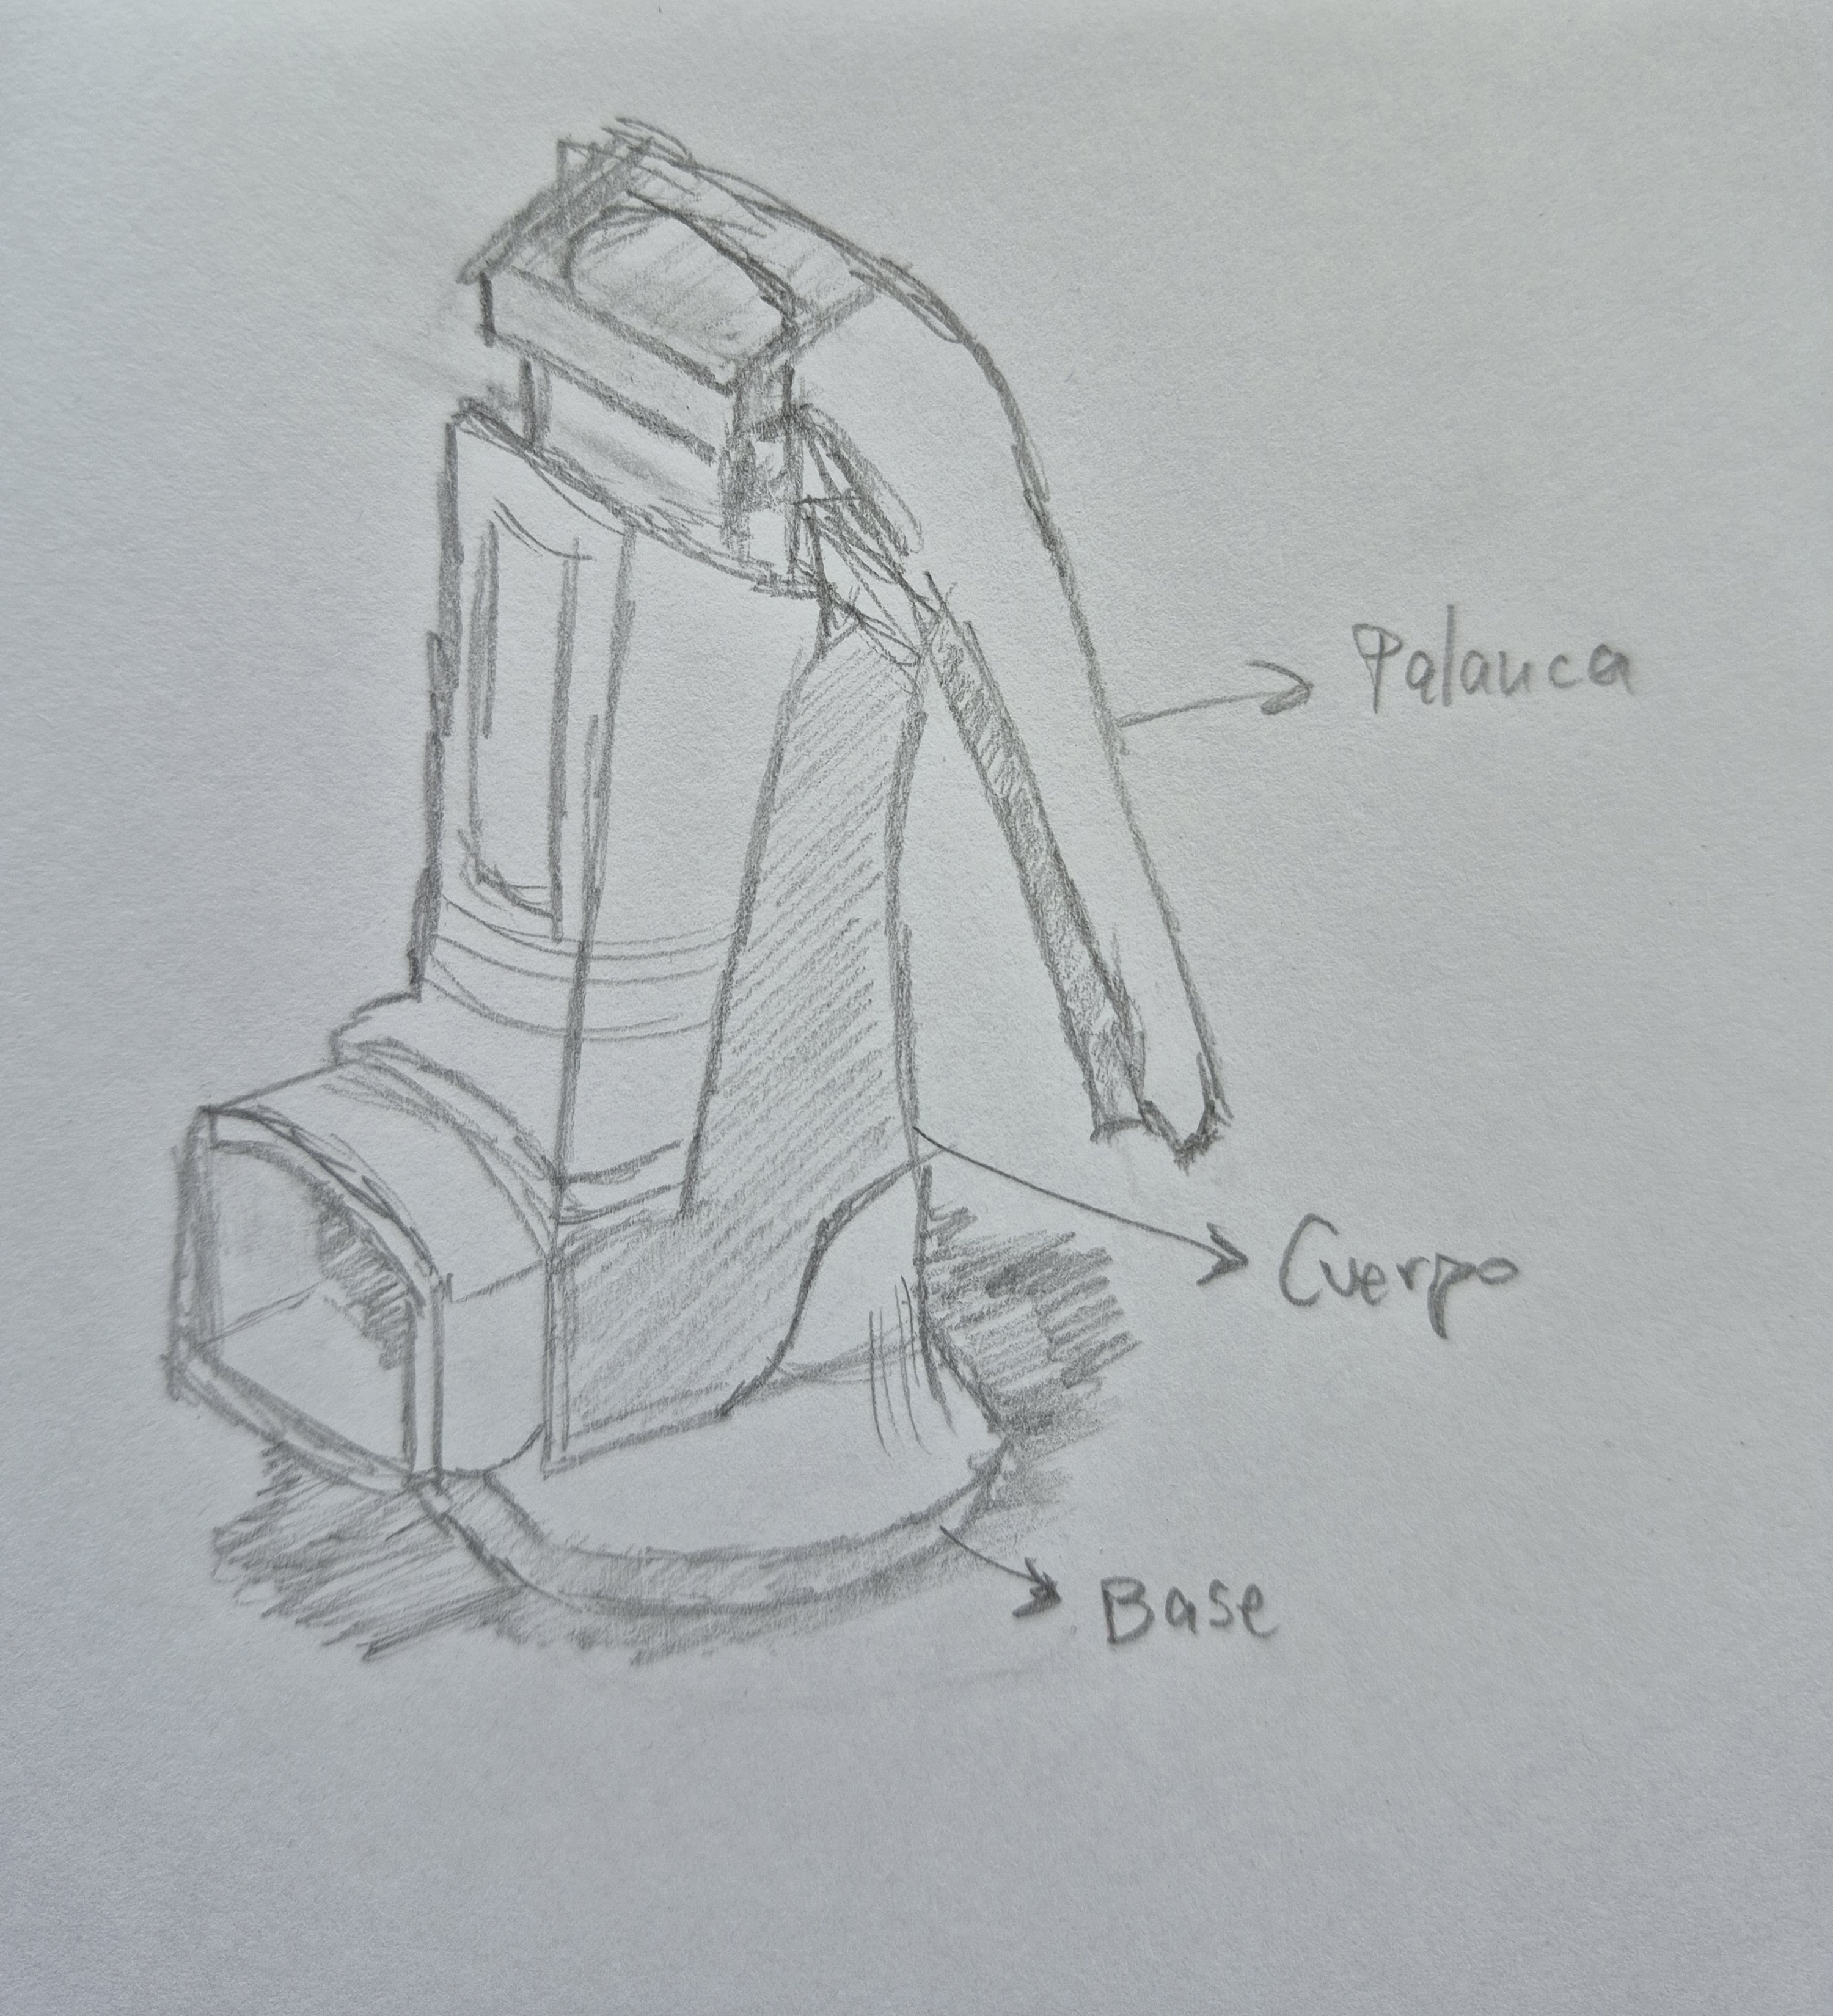
\includegraphics[width=2.8cm, height=2.8cm, keepaspectratio]{boceto_antonio_1.jpg} & 
        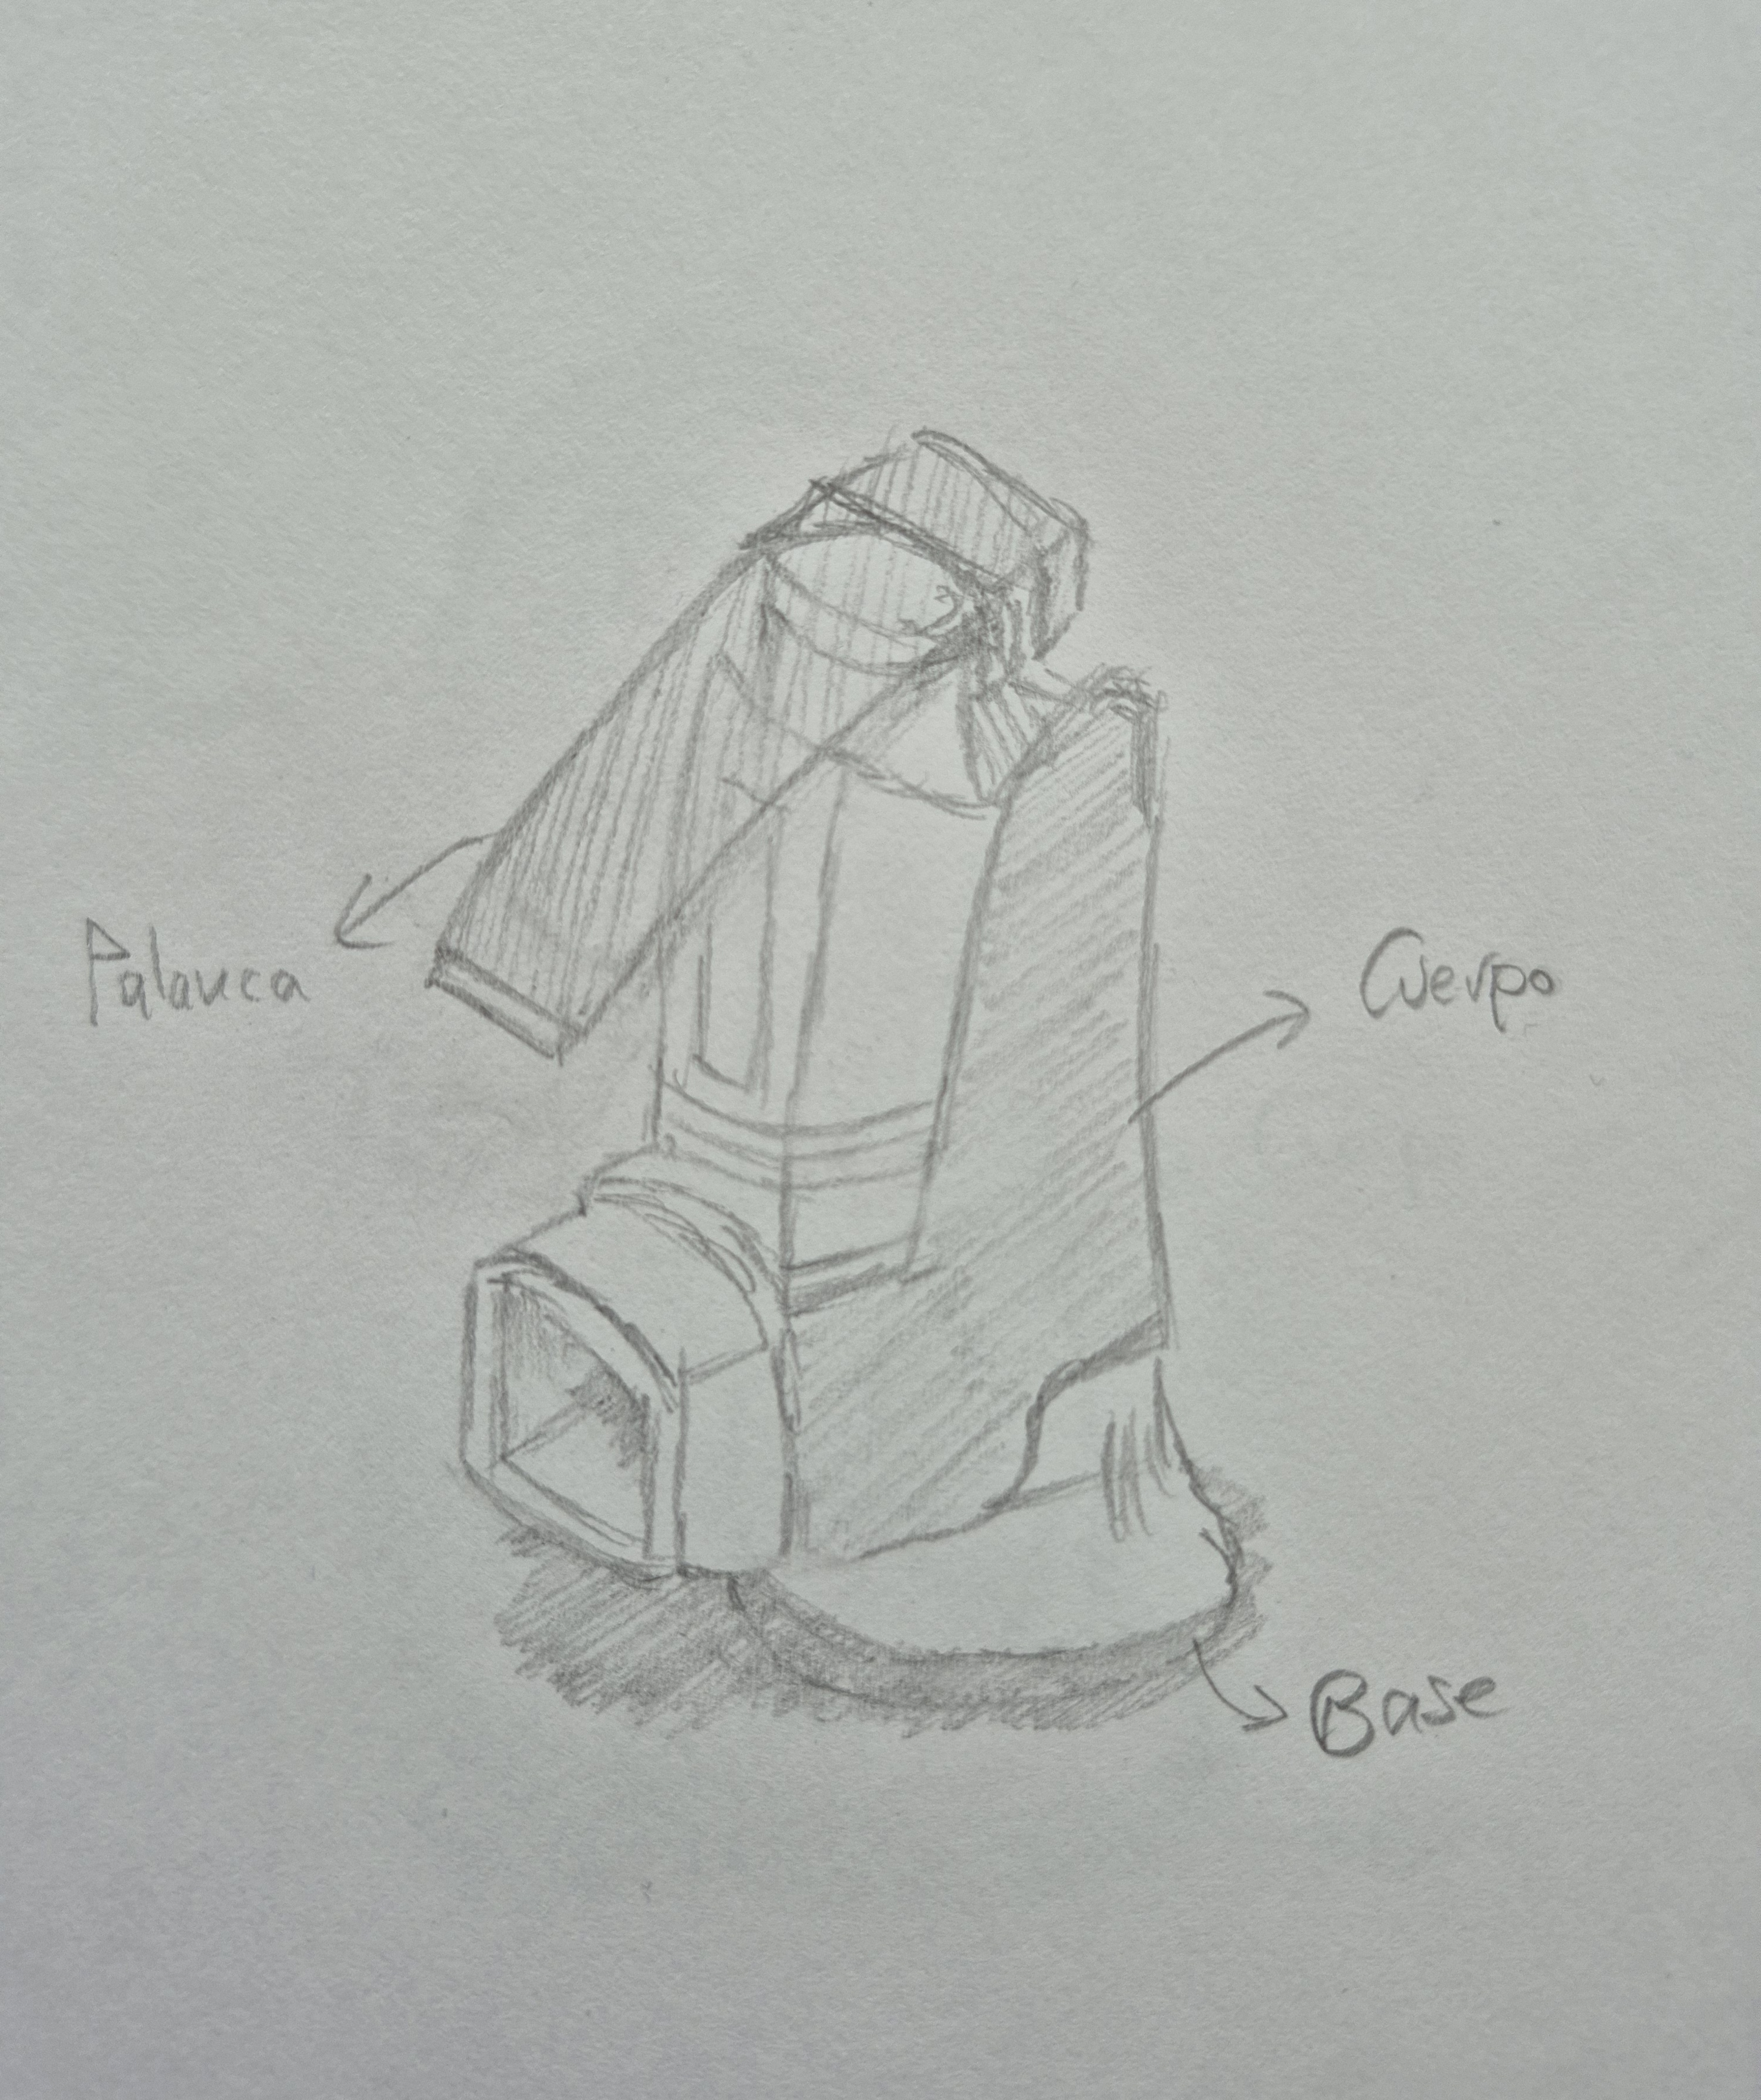
\includegraphics[width=2.8cm, height=2.8cm, keepaspectratio]{boceto_antonio_2.jpg} & 
        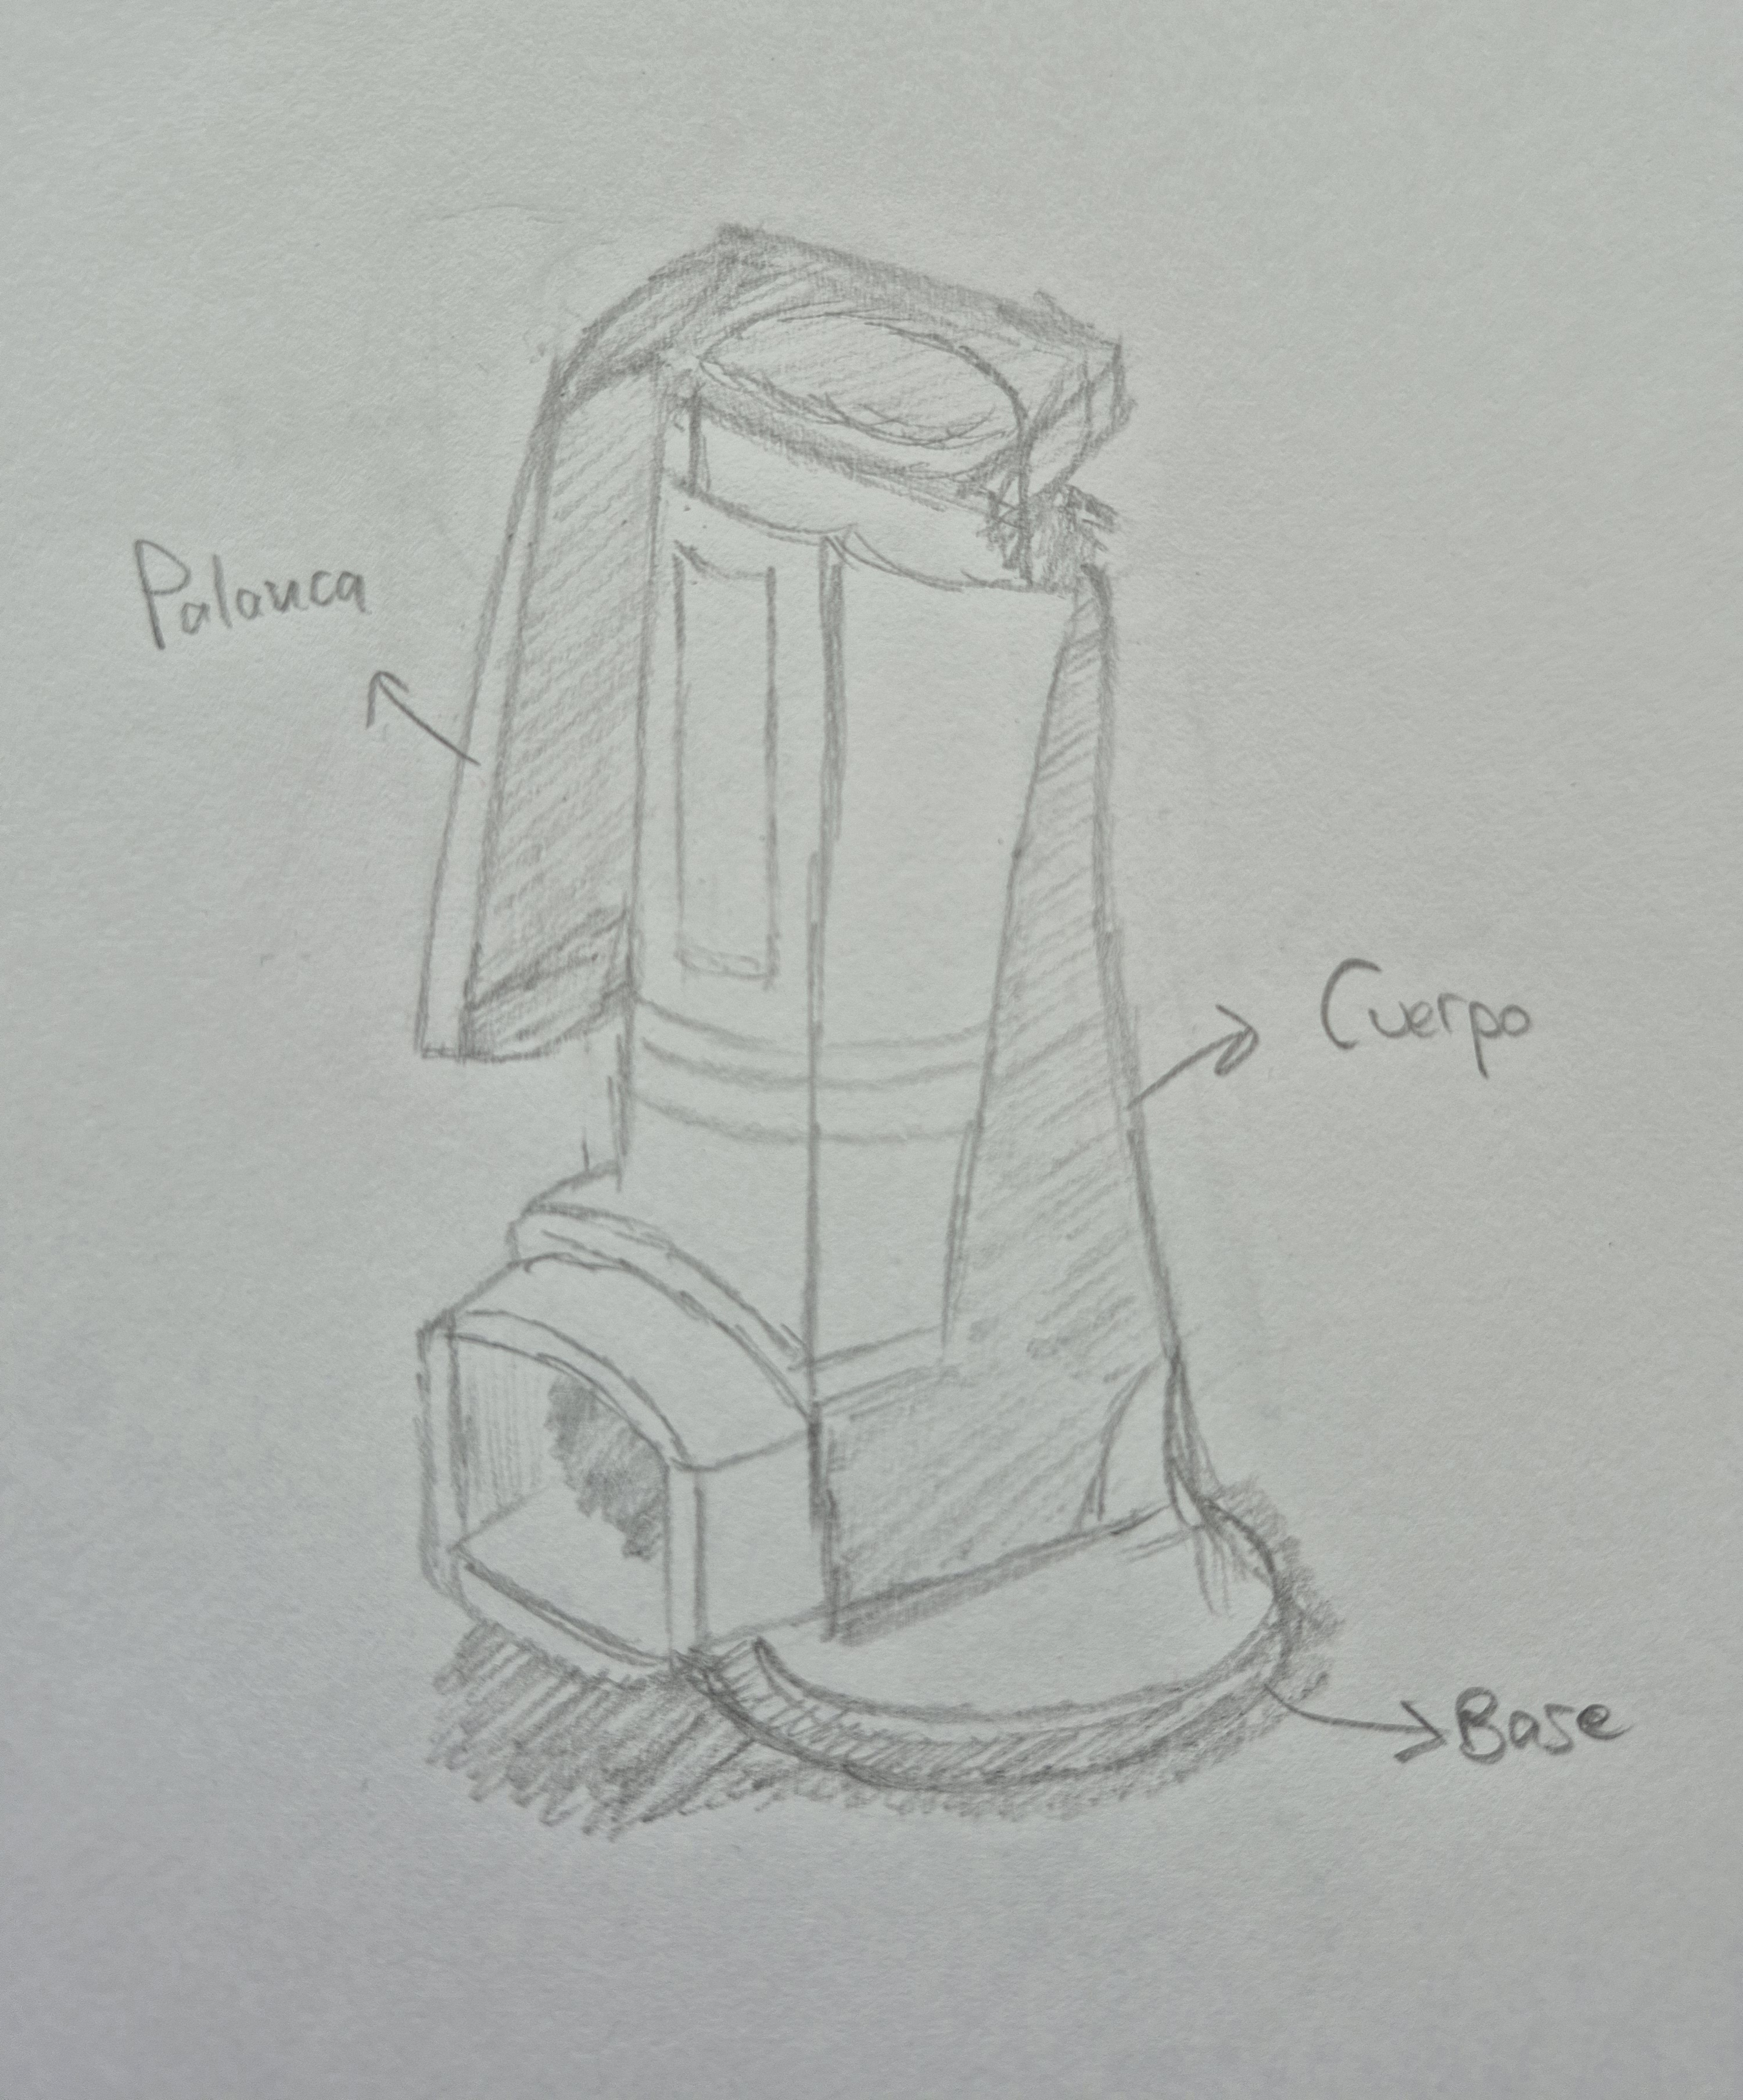
\includegraphics[width=2.8cm, height=2.8cm, keepaspectratio]{boceto_antonio_3.jpg} & 
        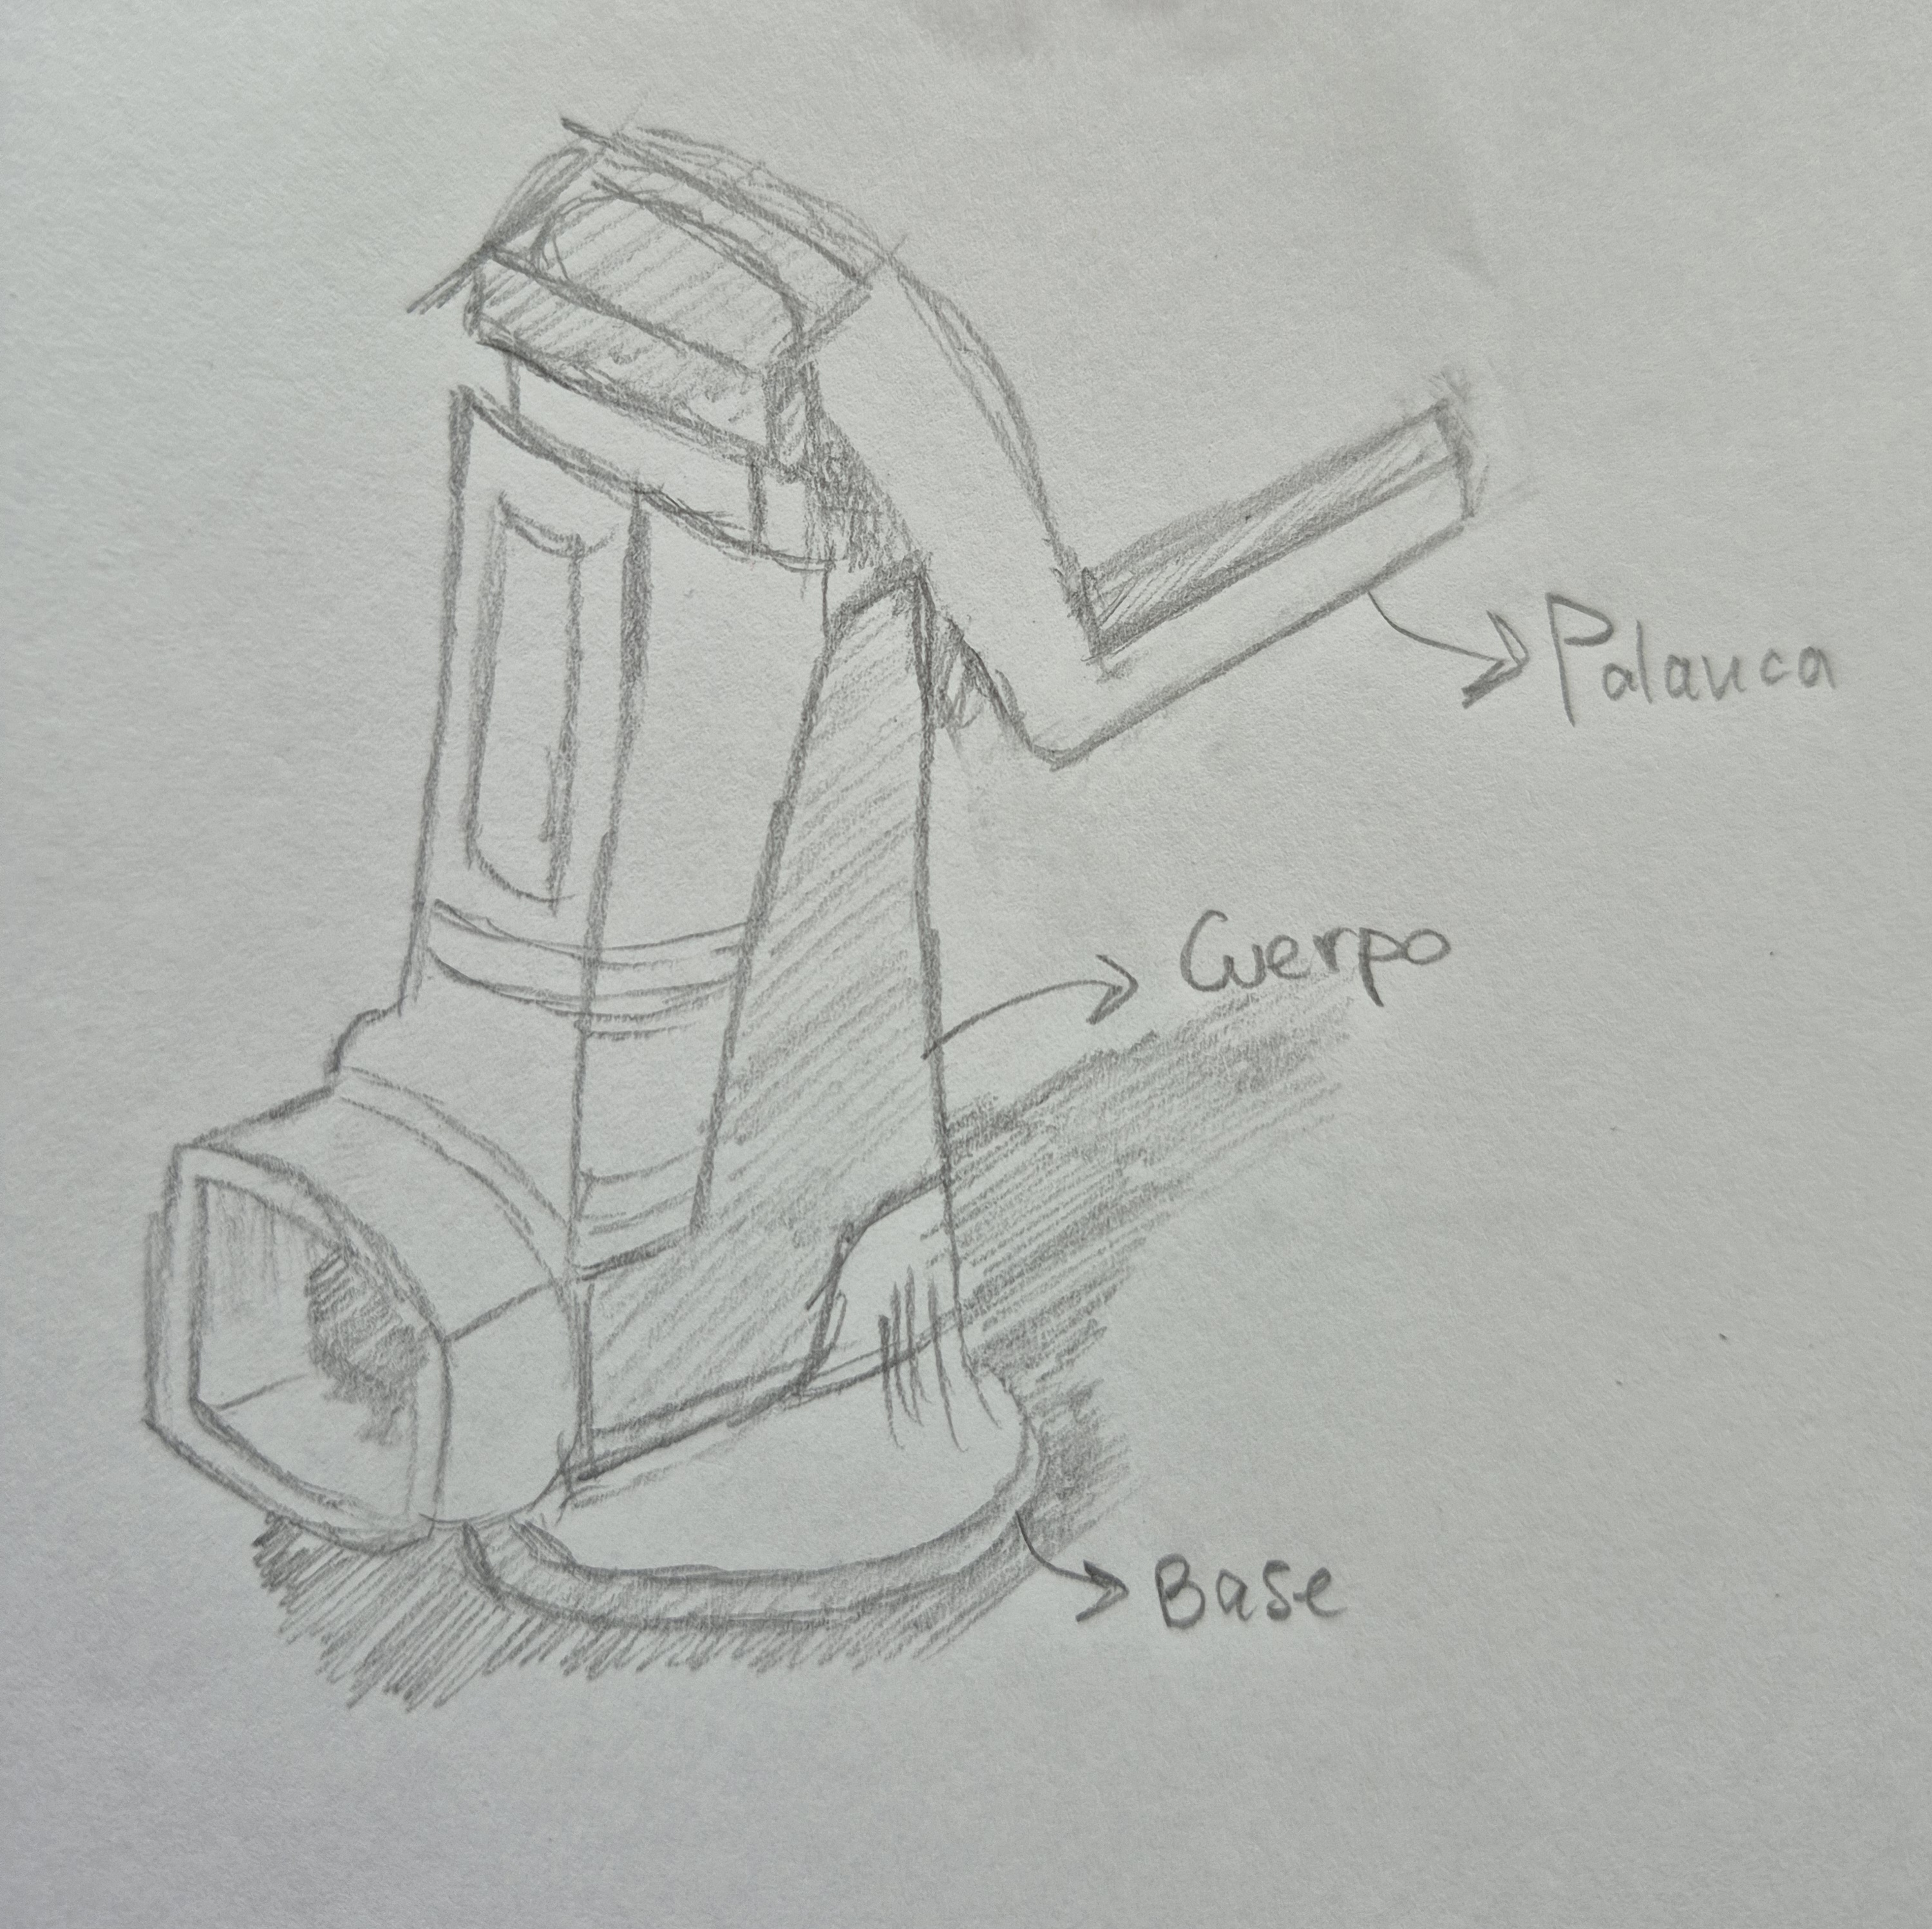
\includegraphics[width=2.8cm, height=2.8cm, keepaspectratio]{boceto_antonio_4.jpg} & 
        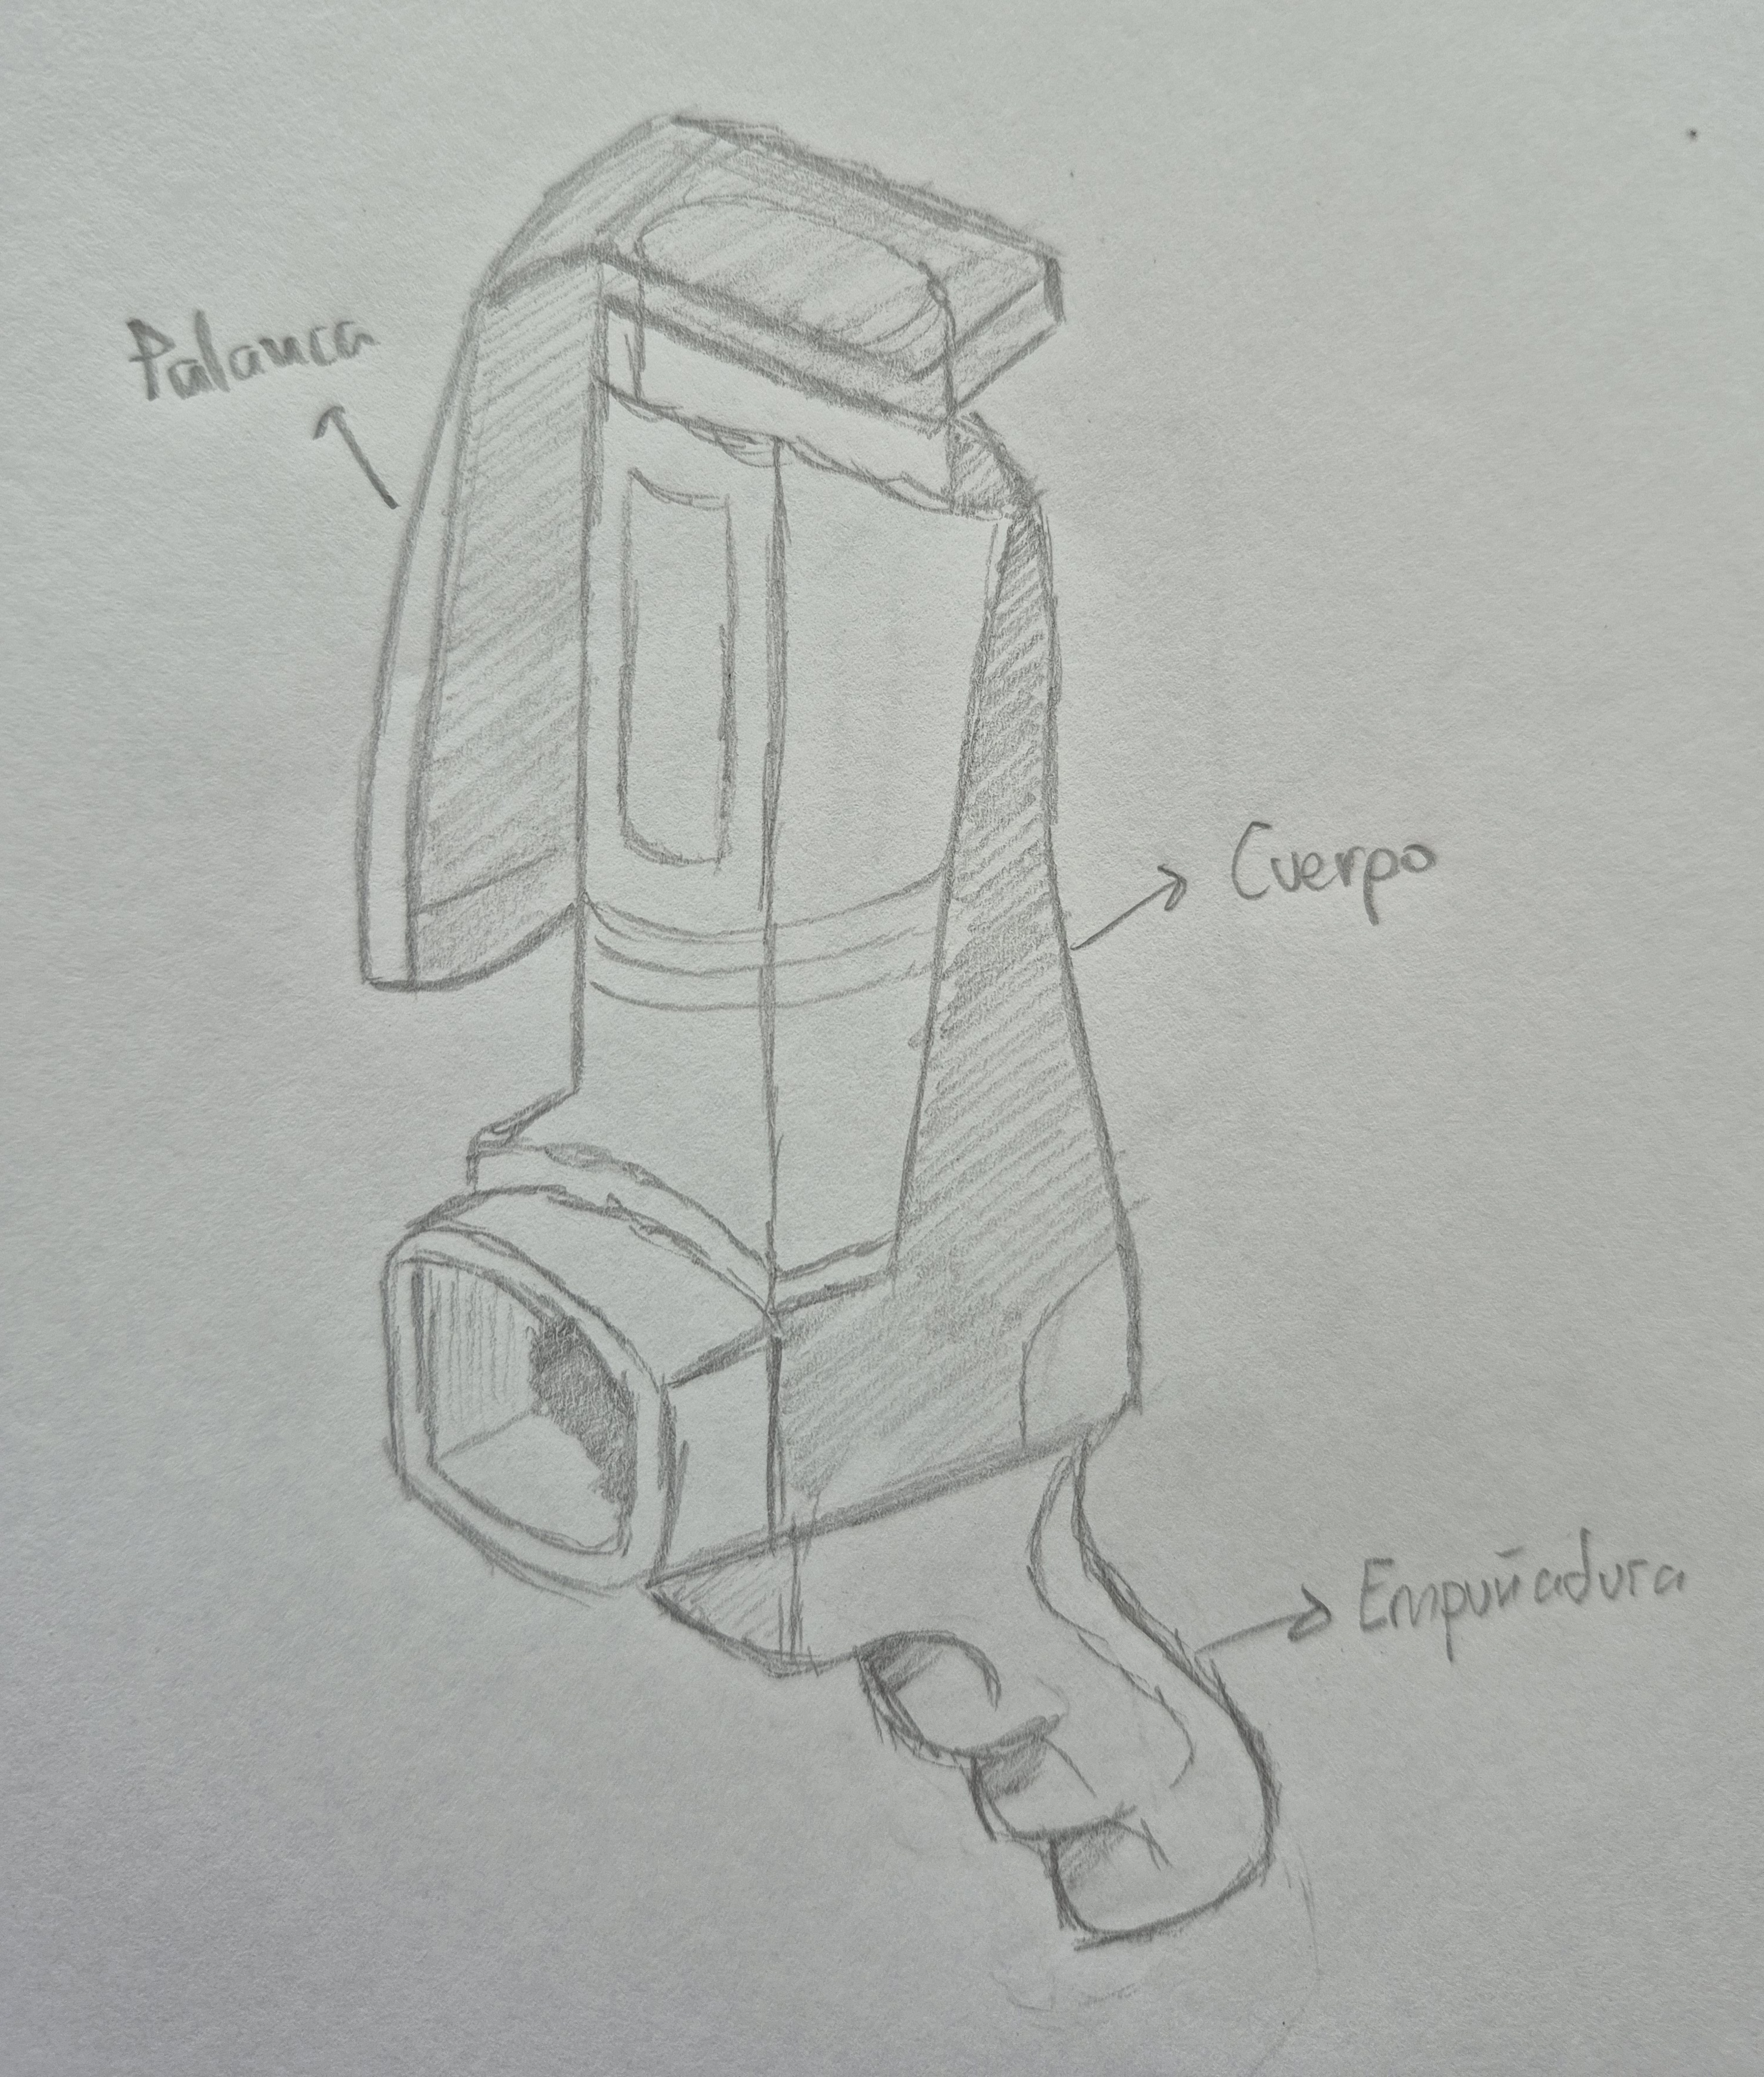
\includegraphics[width=2.8cm, height=2.8cm, keepaspectratio]{boceto_antonio_5.jpg} & 
        
\includegraphics[width=2.8cm, height=2.8cm, keepaspectratio]{ANEXOS/Boceto1_SCM.jpeg} & 
        
\includegraphics[width=2.8cm, height=2.8cm, keepaspectratio]{ANEXOS/Boceto2_SCM.jpeg} & 
        
\includegraphics[width=2.8cm, height=2.8cm, keepaspectratio]{ANEXOS/Boceto3_SCM.jpeg} & 
        
\includegraphics[width=2.8cm, height=2.8cm, keepaspectratio]{ANEXOS/Boceto4_SCM.jpeg} & 
        
\includegraphics[width=2.8cm, height=2.8cm, keepaspectratio]{ANEXOS/Boceto5_SCM.jpeg} & 
        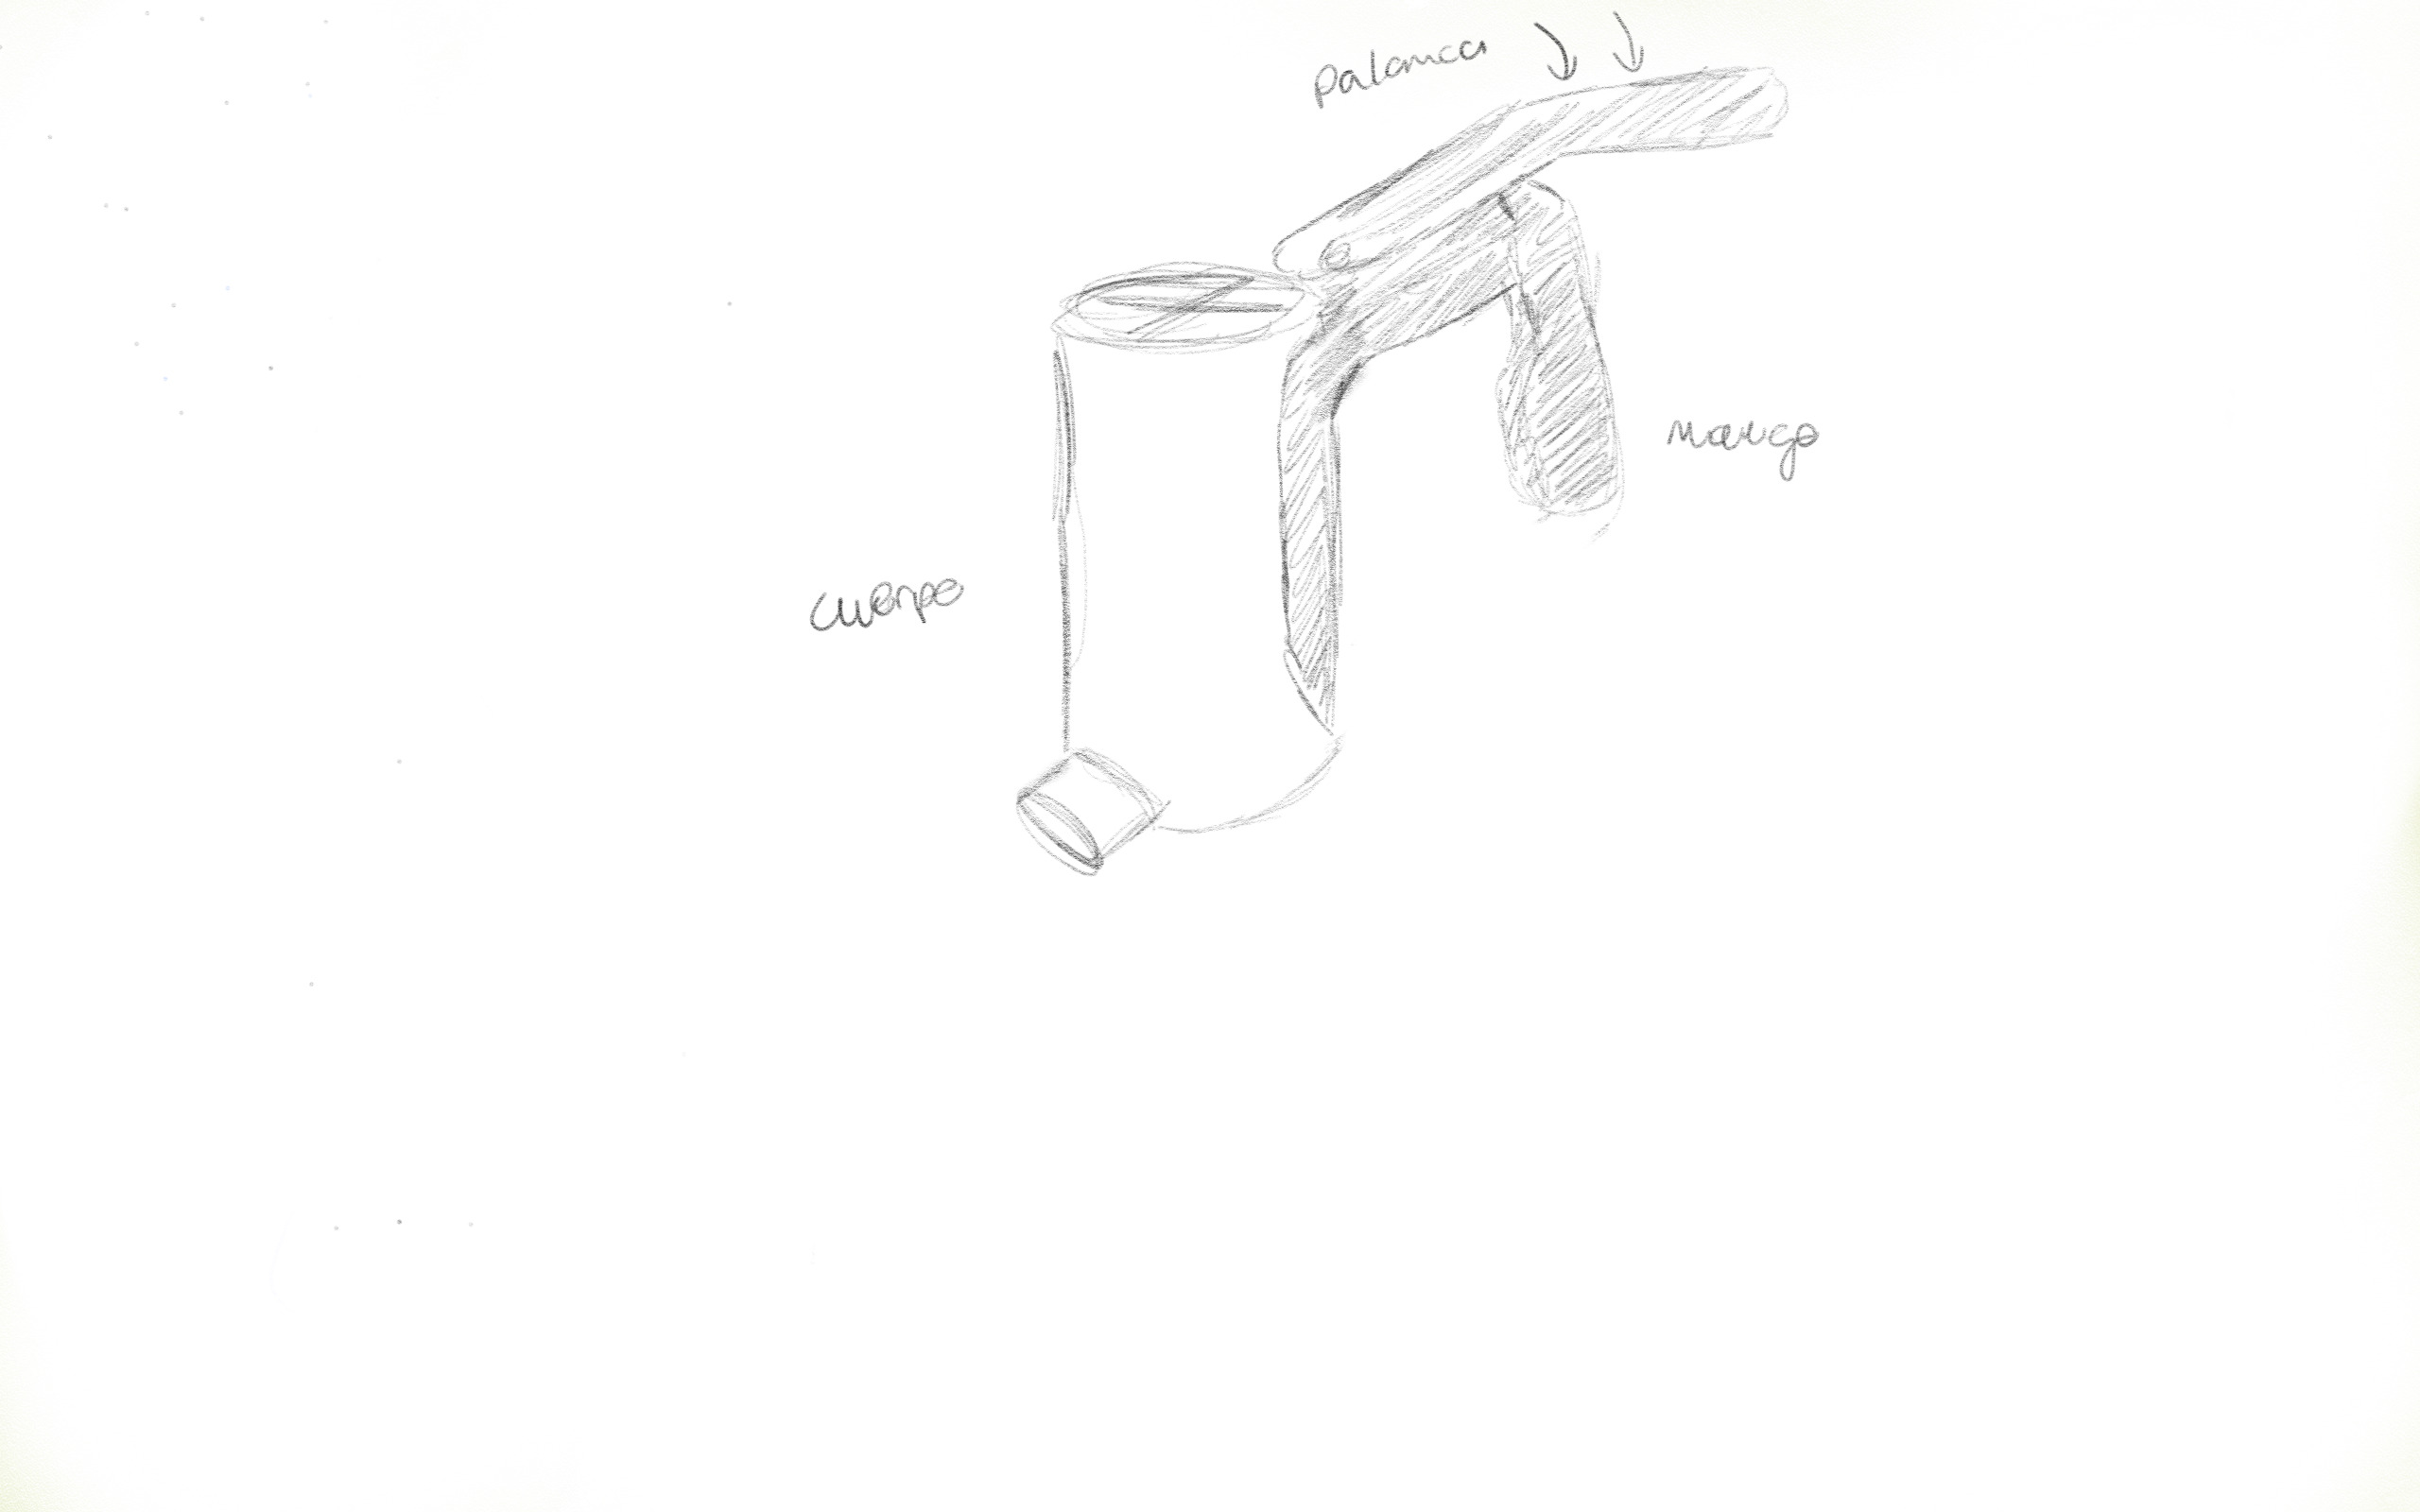
\includegraphics[width=2.8cm, height=2.8cm, keepaspectratio]{boceto_juan_1.jpg} & 
        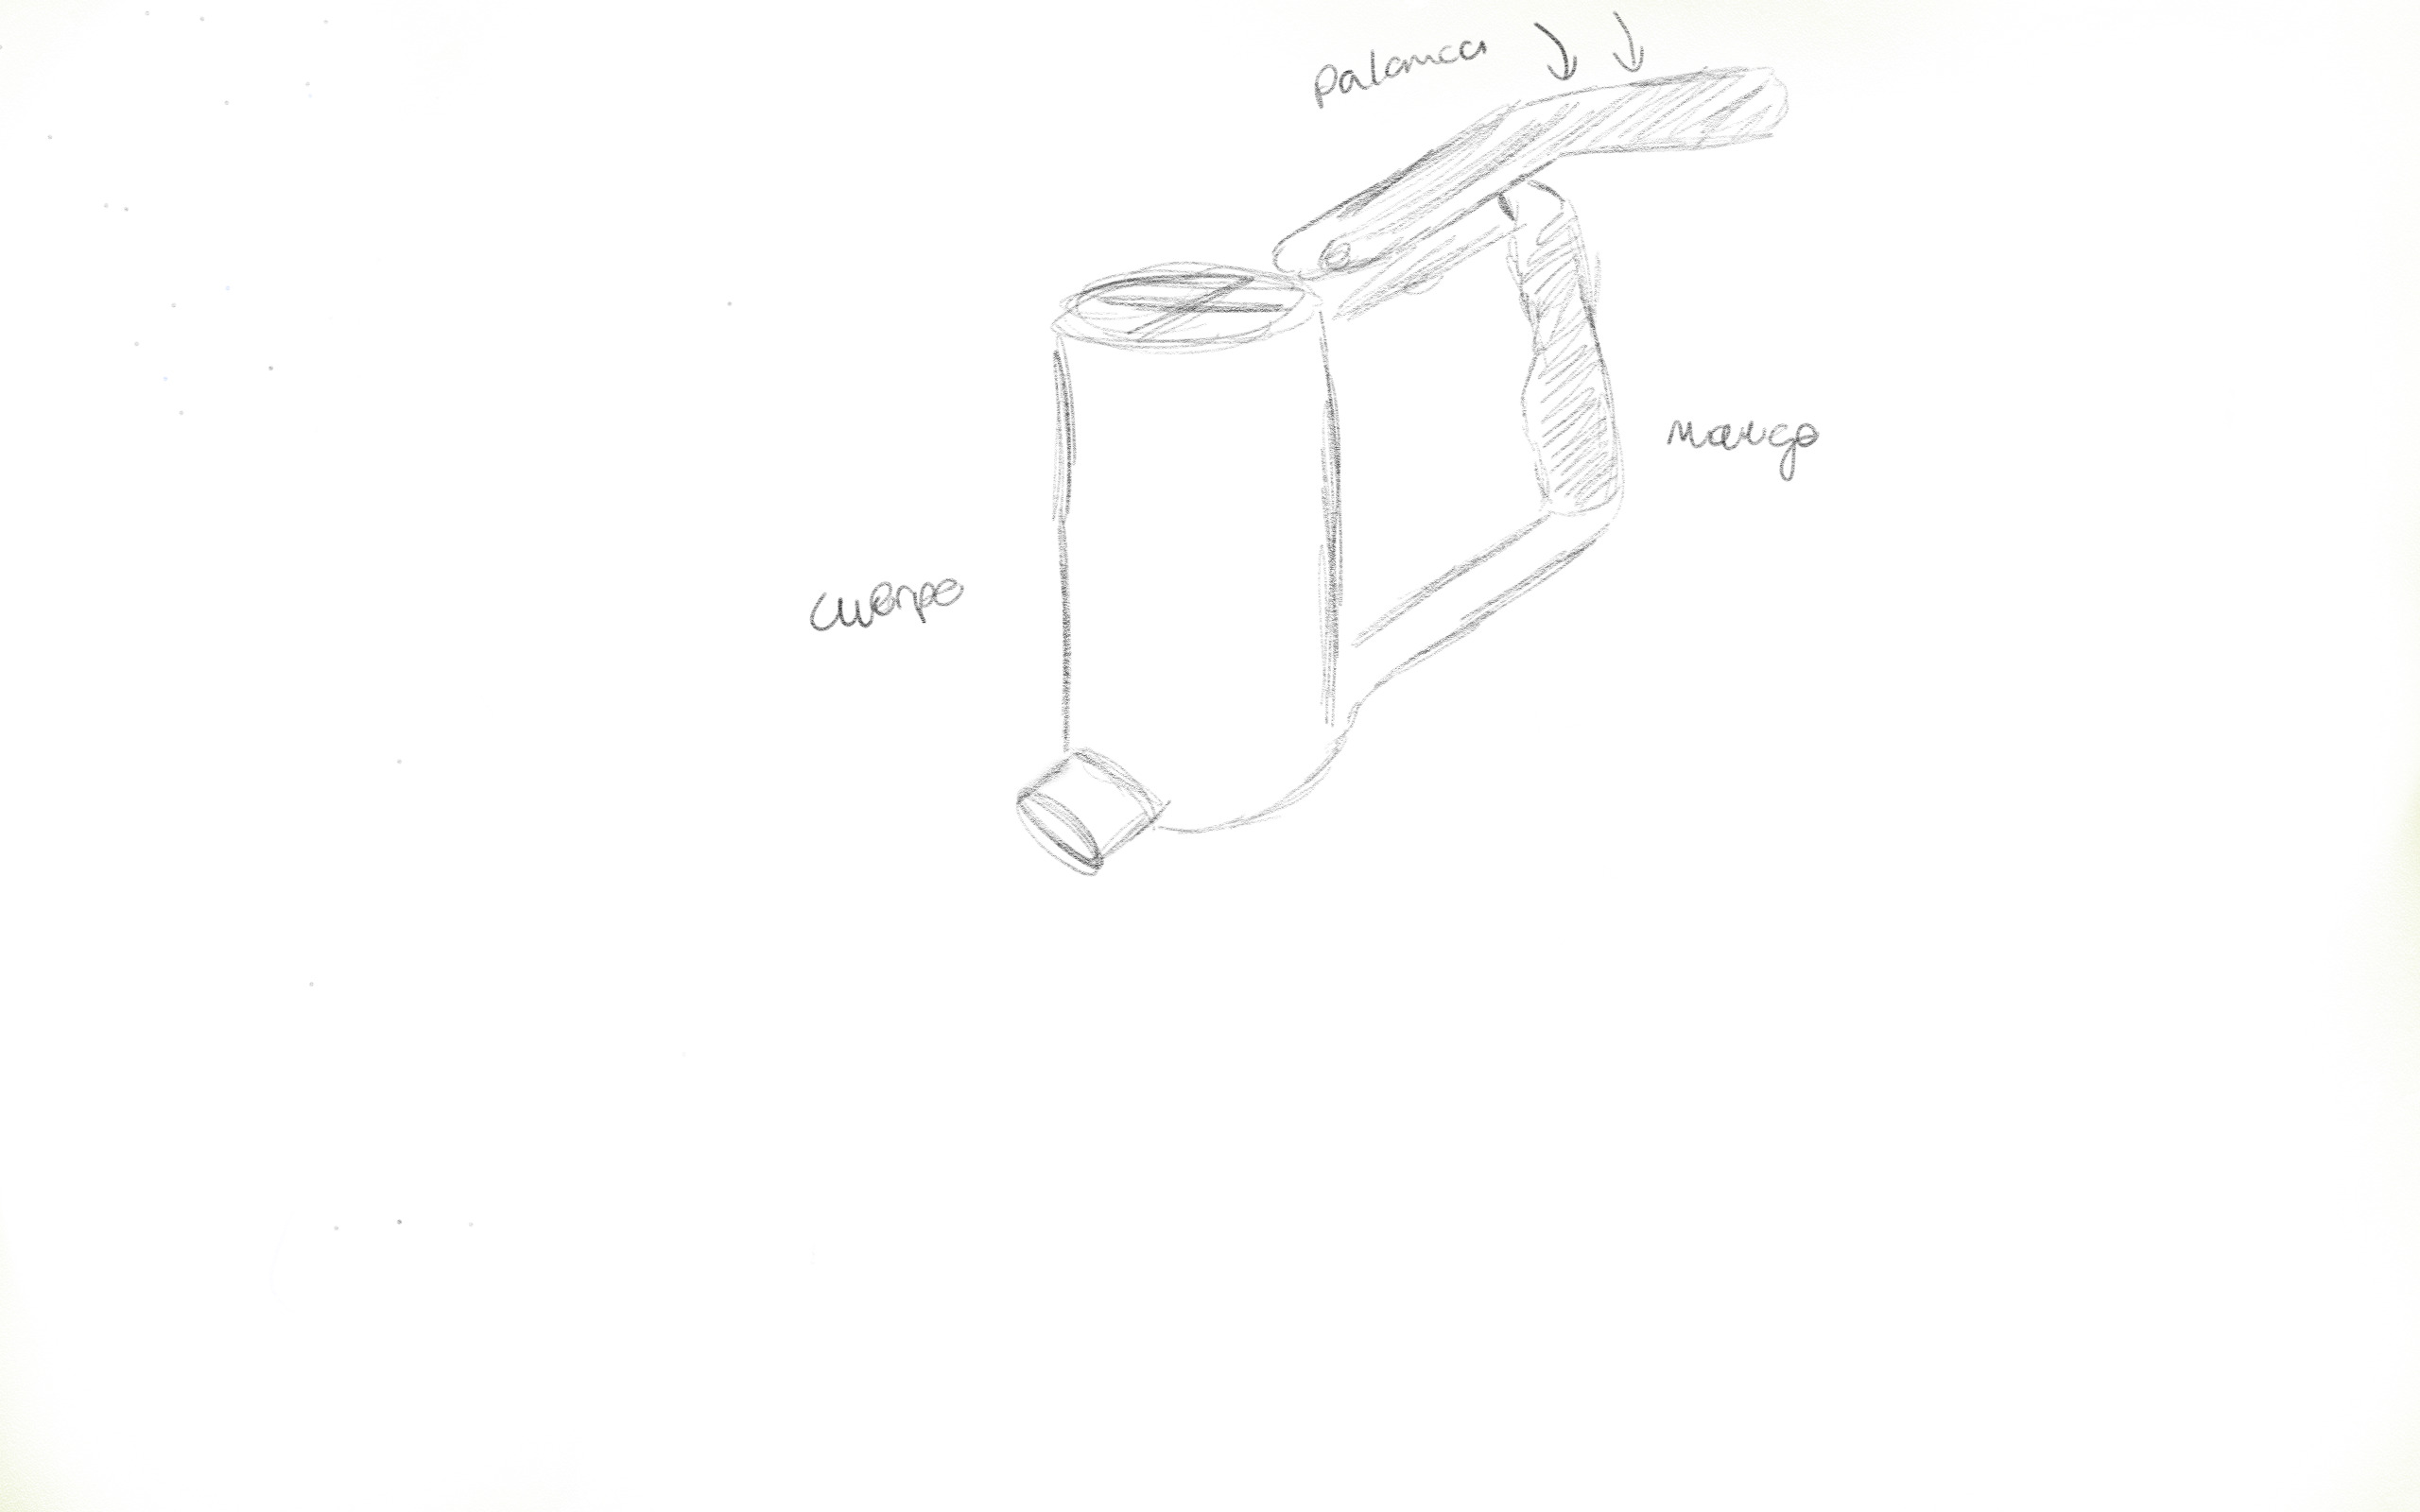
\includegraphics[width=2.8cm, height=2.8cm, keepaspectratio]{boceto_juan_2.jpg} & 
        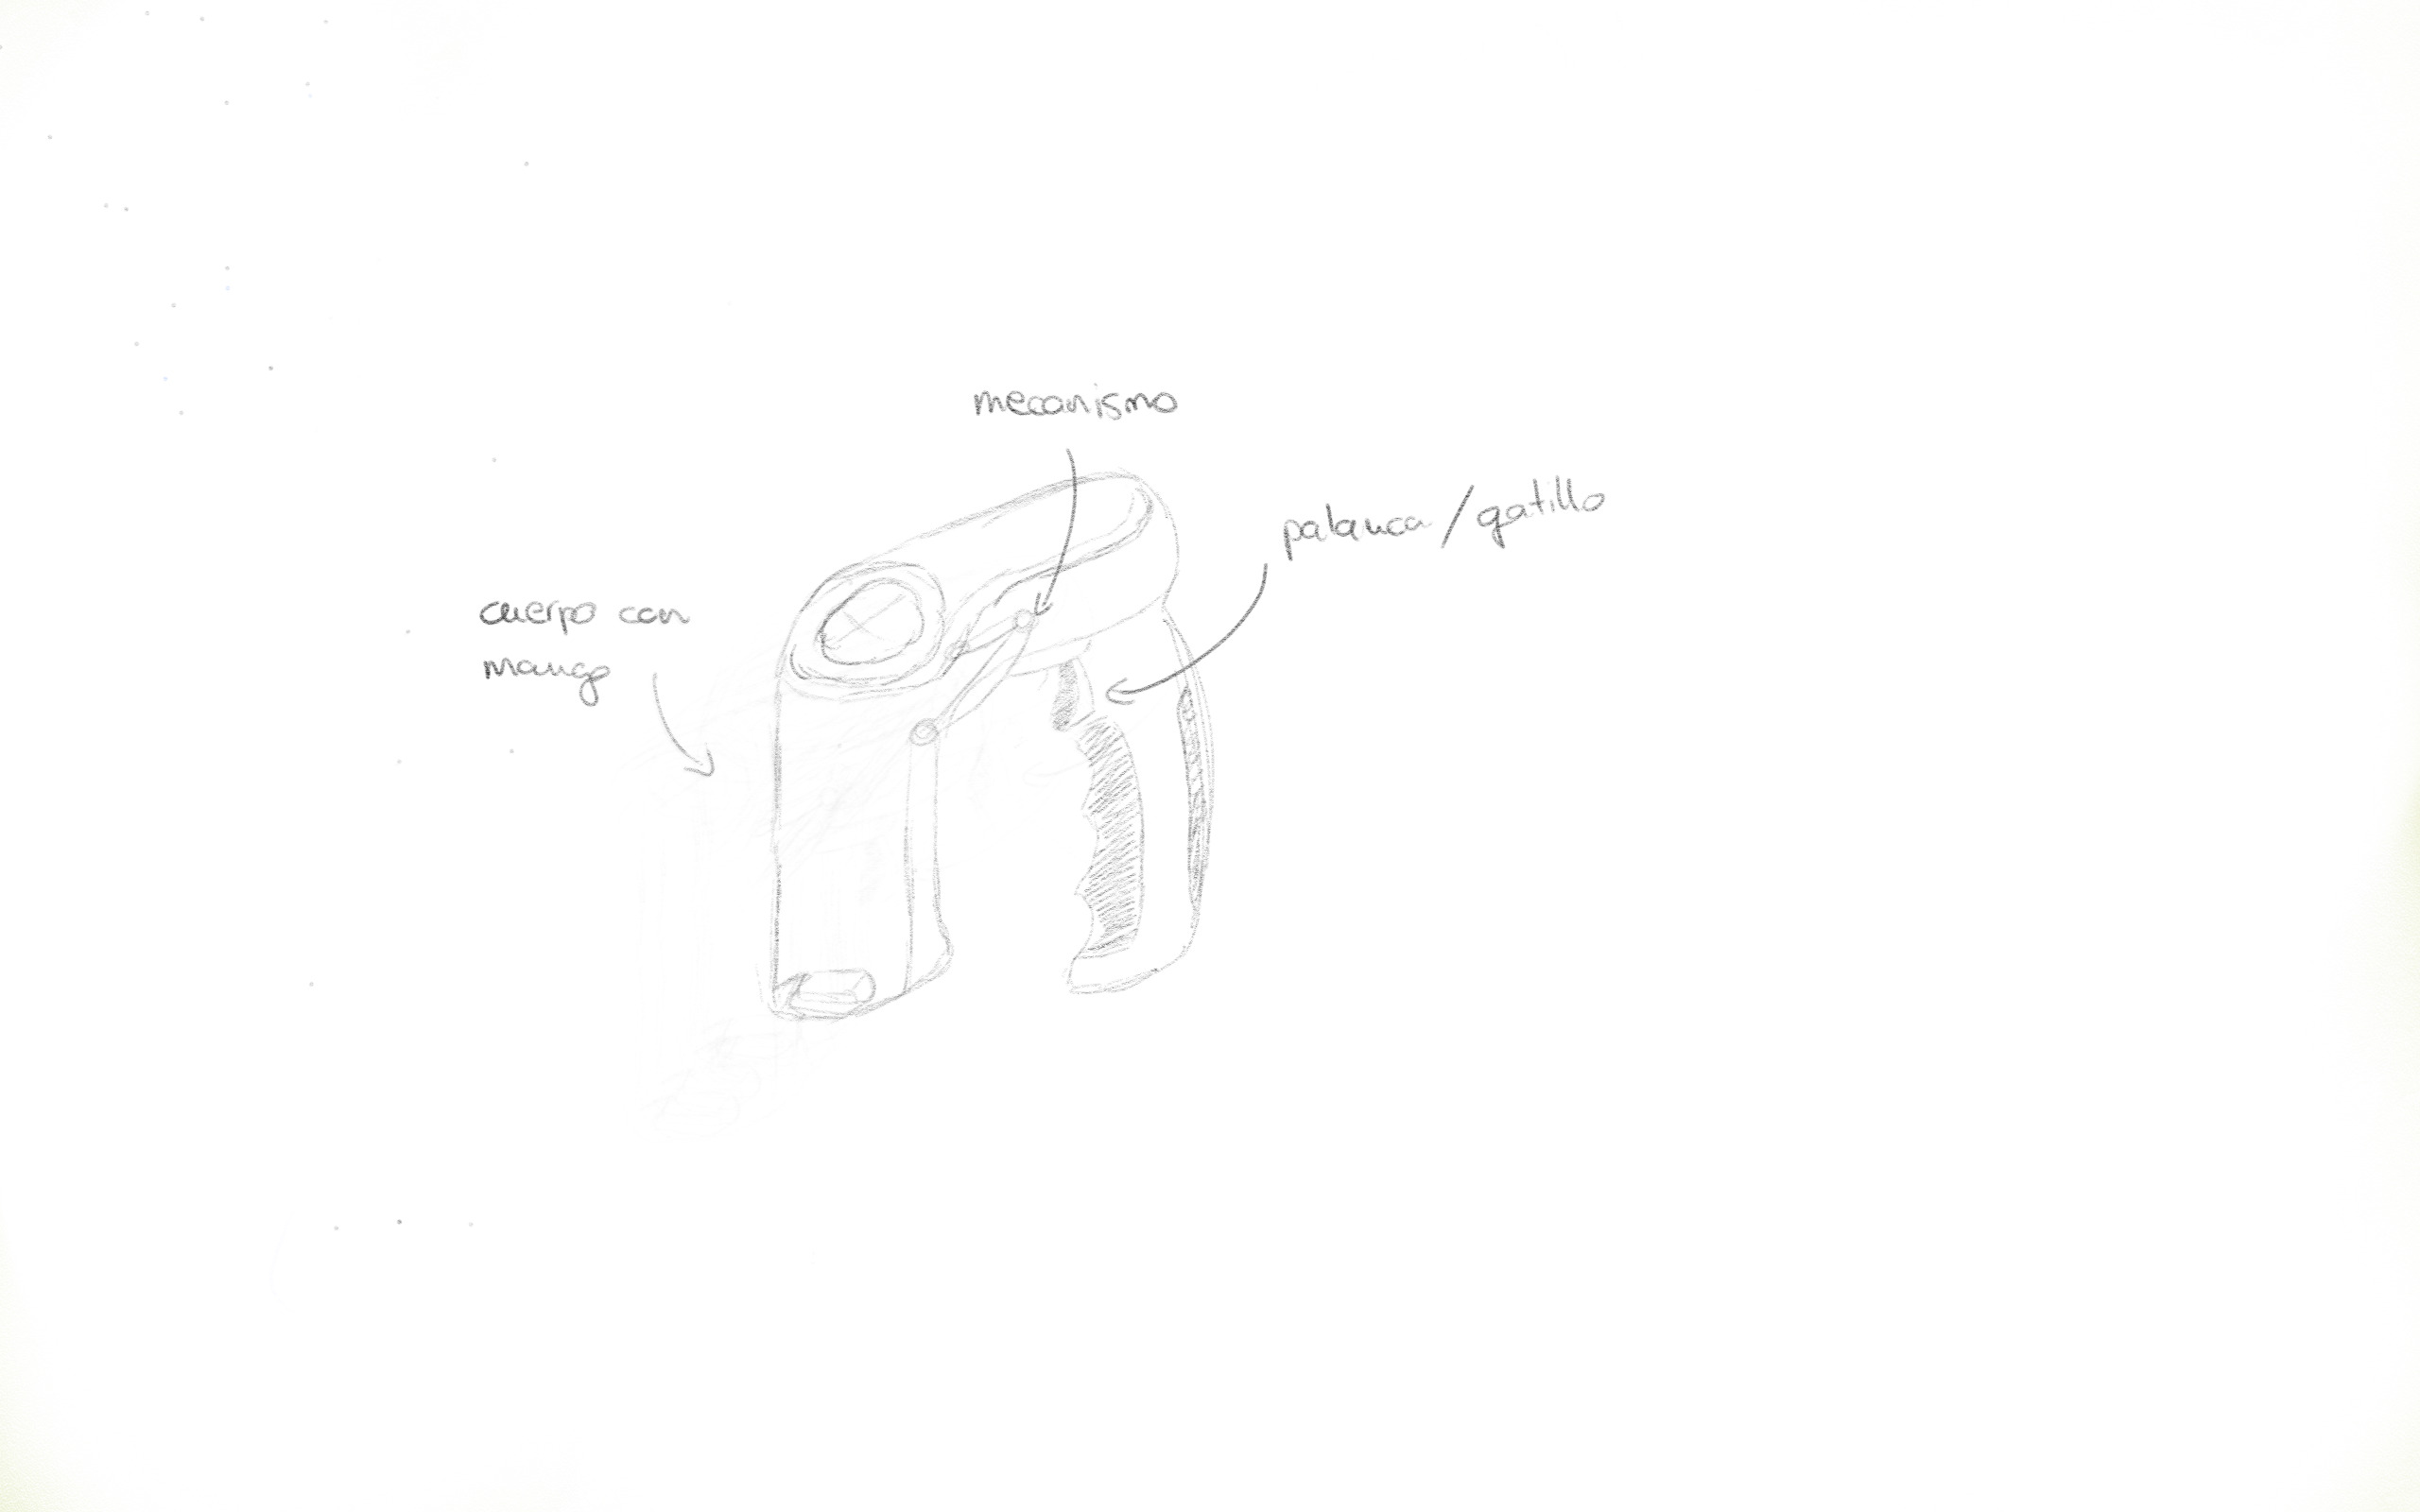
\includegraphics[width=2.8cm, height=2.8cm, keepaspectratio]{boceto_juan_3.jpg} & 
        
\includegraphics[width=2.8cm, height=2.8cm, keepaspectratio]{boceto_juan_4.jpg} & 
        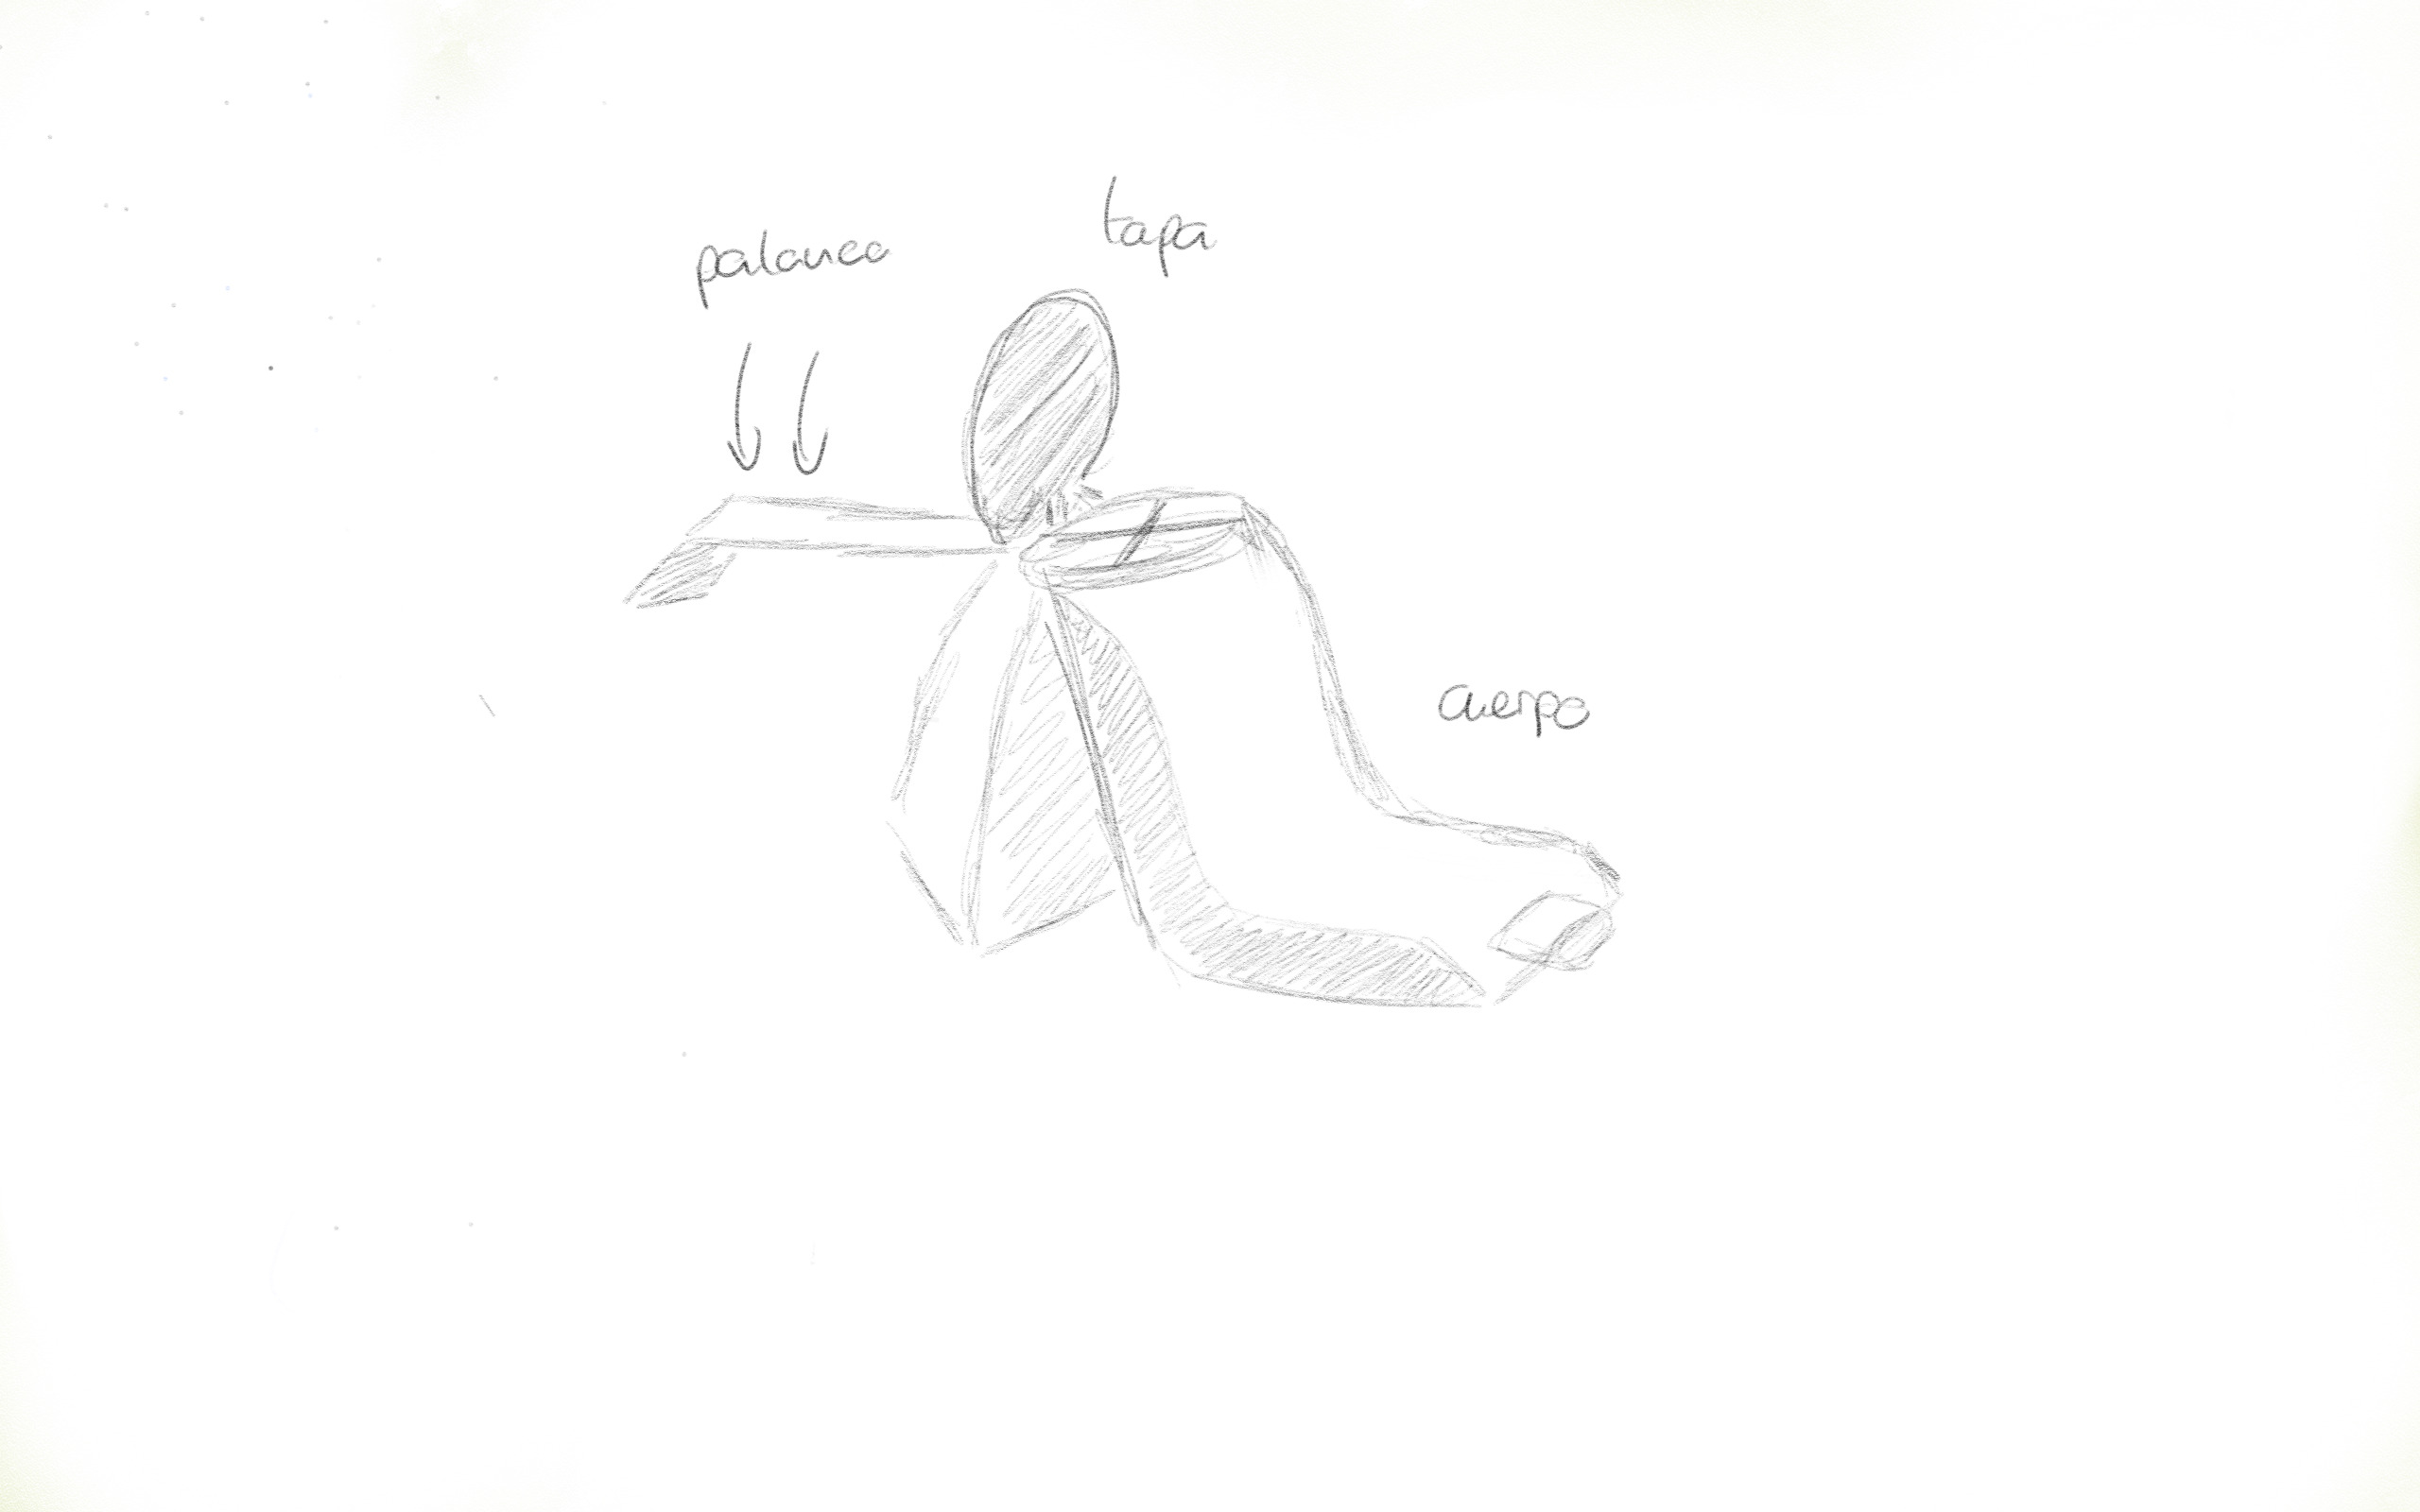
\includegraphics[width=2.8cm, height=2.8cm, keepaspectratio]{boceto_juan_5.jpg} & 
        
\includegraphics[width=2.8cm, height=2.8cm, keepaspectratio]{ANEXOS/Boceto1_Iván.jpeg} & 
        
\includegraphics[width=2.8cm, height=2.8cm, keepaspectratio]{ANEXOS/Boceto2_Iván.jpeg} & 
        
\includegraphics[width=2.8cm, height=2.8cm, keepaspectratio]{ANEXOS/Boceto3_Iván.jpeg} & 
        
\includegraphics[width=2.8cm, height=2.8cm, keepaspectratio]{ANEXOS/Boceto4_Iván.jpeg} & 
        
\includegraphics[width=2.8cm, height=2.8cm, keepaspectratio]{ANEXOS/Boceto5_Iván.jpeg} \\ \hline
        
        % Filas de datos (A-G) con texto resumido
        A. Ergonomía de accionamiento & \huge + & \multirow{7}{*}{\fbox{\textbf{\huge\shortstack{\vspace{4pt}\\D\\A\\T\\U\\M\\\vspace{4pt}}}}} & \huge + & \huge + & \huge S & \huge + & \huge + & \huge + & \huge + & \huge + & \huge + & \huge S & \huge - & \huge - & \huge + & \huge S & \huge + & \huge S & \huge S & \huge S \\ \cline{1-2} \cline{4-21}
        
        B. Fácil montaje & \huge S & & \huge S & \huge S & \huge S & \huge - & \huge S & \huge S & \huge S & \huge S & \huge S & \huge - & \huge - & \huge - & \huge S & \huge - & \huge - & \huge - & \huge - & \huge - \\ \cline{1-2} \cline{4-21}
        
        C. Confort y \newline agarre seguro & \huge + & & \huge + & \huge - & \huge + & \huge + & \huge + & \huge + & \huge + & \huge + & \huge + & \huge S & \huge - & \huge + & \huge - & \huge S & \huge + & \huge - & \huge + & \huge + \\ \cline{1-2} \cline{4-21}
        
        D. Viabilidad de fabricación & \huge S & & \huge S & \huge S & \huge - & \huge - & \huge S & \huge S & \huge - & \huge S & \huge S & \huge S & \huge - & \huge S & \huge - & \huge - & \huge - & \huge - & \huge - & \huge - \\ \cline{1-2} \cline{4-21}
        
        E. Facilidad de limpieza & \huge S & & \huge S & \huge S & \huge S & \huge - & \huge - & \huge S & \huge S & \huge - & \huge - & \huge - & \huge - & \huge - & \huge - & \huge S & \huge S & \huge S & \huge S & \huge S \\ \cline{1-2} \cline{4-21}
        
        F. Uso autónomo  & \huge + & & \huge S & \huge S & \huge S & \huge S & \huge S & \huge S & \huge S & \huge S & \huge S & \huge S & \huge S & \huge S & \huge S & \huge S & \huge S & \huge S & \huge S & \huge S \\ \cline{1-2} \cline{4-21}

        G. Estética e \newline identidad visual & \huge S & & \huge S & \huge + & \huge + & \huge S & \huge S & \huge S & \huge S & \huge S & \huge S & \huge S & \huge + & \huge S & \huge S & \huge S & \huge S & \huge + & \huge S & \huge + \\ \hline
        
        % Sumatorios
        \rowcolor{gray!10}
        \textbf{\huge Total +} & \huge 3 & & \huge 2 & \huge 2 & \huge 2 & \huge 2 & \huge 2 & \huge 2 & \huge 2 & \huge 2 & \huge 2 & \huge 0 & \huge 1 & \huge 1 & \huge 1 & \huge 0 & \huge 2 & \huge 1 & \huge 1 & \huge 2 \\ \hline
        \rowcolor{gray!10}
        \textbf{\huge Total -} & \huge 0 & & \huge 0 & \huge 1 & \huge 1 & \huge 3 & \huge 1 & \huge 0 & \huge 1 & \huge 1 & \huge 1 & \huge 2 & \huge 5 & \huge 3 & \huge 3 & \huge 2 & \huge 2 & \huge 3 & \huge 2 & \huge 2 \\ \hline
    \end{tabular}
    }
    \vspace{0.4cm}
    \caption{Matriz de selección de conceptos con descripción de criterios.}
    \label{tab:matriz_pugh_grande}
\end{table}
\vspace*{\fill}
\end{landscape}

\vspace{0.5cm}


\vspace{1cm}

\begin{figure}[H]
    \centering
    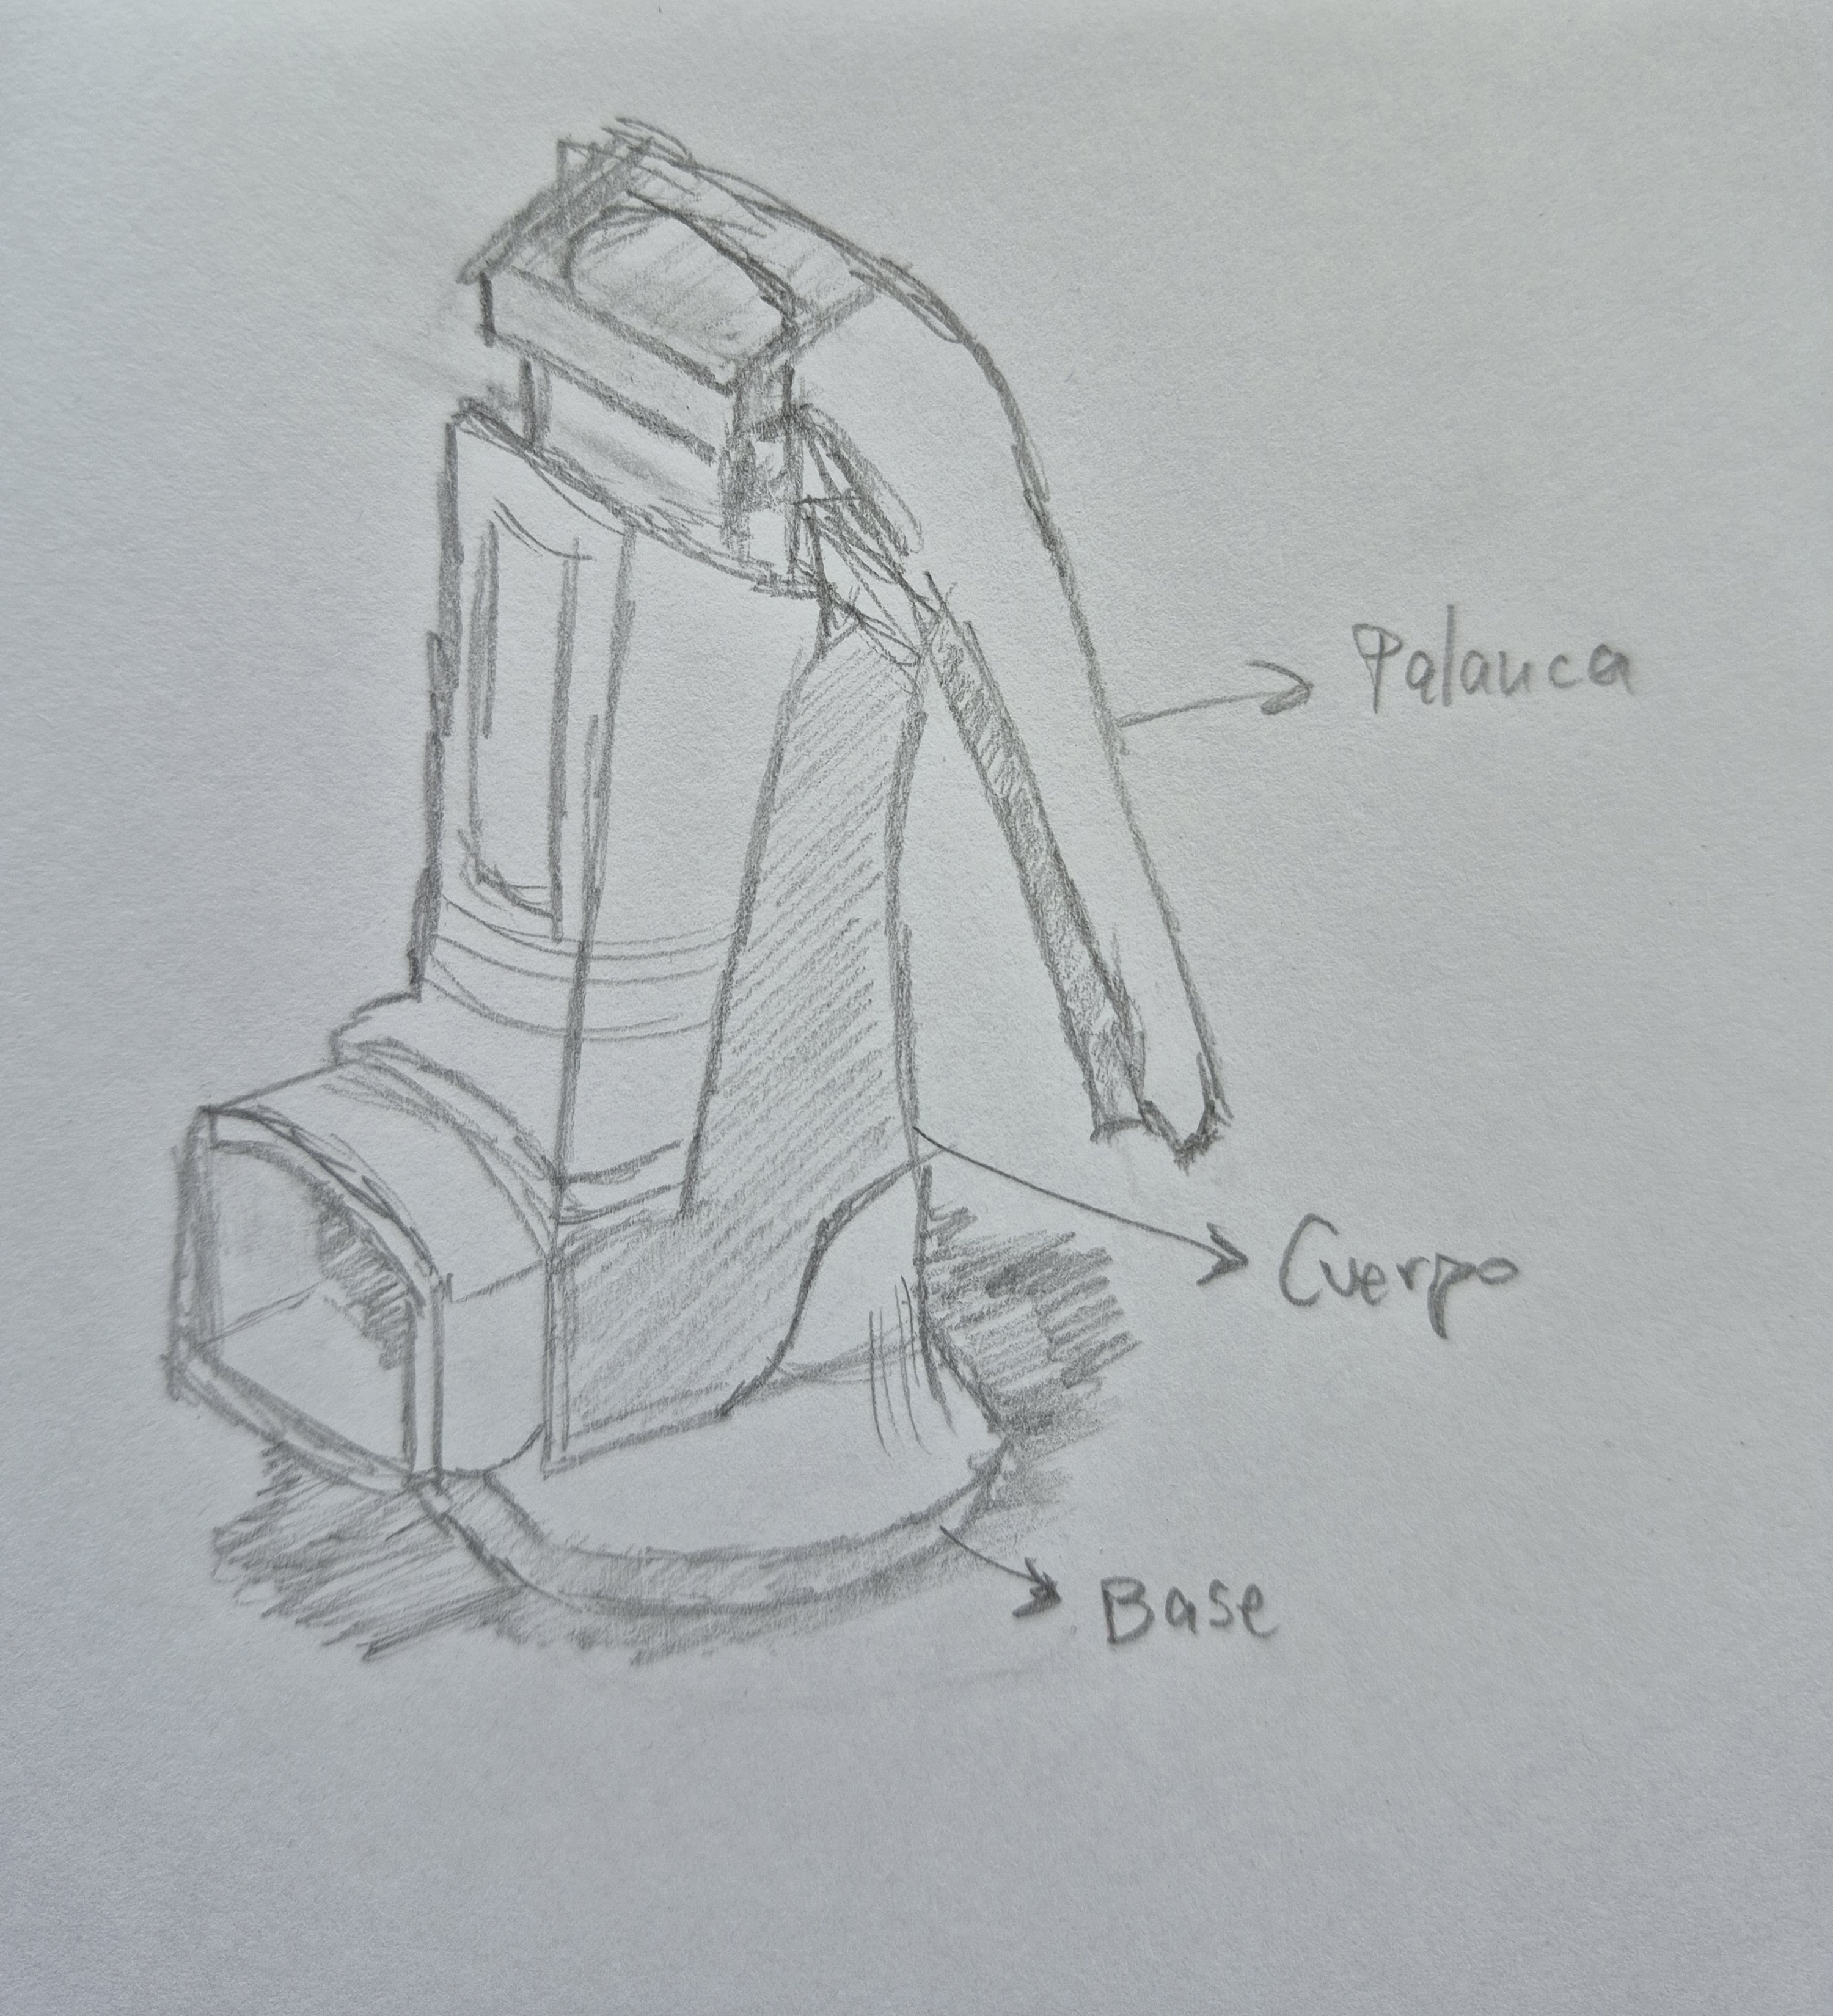
\includegraphics[width=0.8\textwidth]{boceto_antonio_1.jpg}
    \caption{Diseño conceptual seleccionado para su desarrollo mediante la matriz de Pugh. \centering Boceto NÚMERO 1 del proyectista D. ANTONIO SÁNCHEZ DOÑA}
    \label{fig:seleccion_final}
\end{figure}



% ======================================================
% BLOQUE DE FIRMAS
% ======================================================
\noindent\begin{minipage}{\textwidth}
    \begin{flushright}
        En Málaga, a \today
    \end{flushright}
    \vspace{2cm}

    \noindent
    \begin{minipage}[t]{0.45\textwidth}
        \centering
        \rule{6cm}{0.6pt} \\
        \textbf{Fdo. D. Sergio Carmona Muñoz} \\
        Colegiado Nº 06424 \\
        DNI: 26291930D
    \end{minipage}
    \hfill
    \begin{minipage}[t]{0.45\textwidth}
        \centering
        \rule{6cm}{0.6pt} \\
        \textbf{Fdo. D. Juan Gabriel Navarro Valdivielso} \\
        Colegiado Nº 06425 \\
        DNI: 77666662D
    \end{minipage}

    \vspace{2cm}

    \noindent
    \begin{minipage}[t]{0.45\textwidth}
        \centering
        \rule{6cm}{0.6pt} \\
        \textbf{Fdo. D. Antonio Sánchez Doña} \\
        Colegiado Nº 06423 \\
        DNI: 79380534J
    \end{minipage}
    \hfill
    \begin{minipage}[t]{0.45\textwidth}
        \centering
        \rule{6cm}{0.6pt} \\
        \textbf{Fdo. D. Iván de la Torre Segato} \\
        Colegiado Nº 06421 \\
        DNI: 79383630G
    \end{minipage}
\end{minipage}
\vspace{1cm}

% ======================================================
% HOJA EN BLANCO CON MARCA DE AGUA
% ======================================================
\newpage
\pagestyle{fancy}

\begin{tikzpicture}[remember picture, overlay]
    \node[opacity=0.1] at (current page.center) {
\includegraphics[width=12cm]{logo_definitivo.png}};
\end{tikzpicture}

% Empujamos el texto hacia la parte inferior del folio
\vspace*{8.5cm} 
\begin{center}
    \textit{Esta hoja ha sido dejada deliberadamente en blanco.}
\end{center}
\vfill

\end{document}